\documentclass{article}
\usepackage{lipsum}
\usepackage[hidelinks]{hyperref}
\usepackage{graphicx}

\begin{document}

% Title
\title{Certificats et documents justificatifs}
\author{Mehdi JAFARIZADEH}
\date{\today}
\maketitle

% Table of Contents
\tableofcontents


% =========================================================
% ===================== Introduction ======================
% =========================================================

\newpage
\section{Introduction}
Bienvenue dans la documentation complète de mes réalisations académiques et professionnelles. Ce dossier encapsule un enregistrement détaillé de mon parcours éducatif, de mon expérience professionnelle, de mes certifications et de mes contributions à divers domaines académiques et professionnels. Chaque section de ce document est méticuleusement organisée pour fournir un aperçu clair et complet de mes qualifications et réalisations.

Pour faciliter l'accès et atteindre un public plus large, ce document est disponible en Anglais et en Français. Si vous préférez consulter la version Anglaise, vous pouvez y accéder via le lien suivant : \href{https://drive.google.com/file/d/1SwrSxWrC8iVVY-hpDYJElf16-4BYZWbR/view?usp=drive_link}{[Lien vers la version Anglaise}.

Tout au long de ce document, vous trouverez des descriptions détaillées de mes réalisations, y compris des liens vers les certificats pertinents et les documents de soutien, garantissant une transparence totale et une facilité de vérification pour toutes les affirmations énoncées.

Ce document est conçu pour être navigable et interactif, avec des liens cliquables qui mènent à des descriptions détaillées et à des représentations numériques de certificats, de récompenses et de lettres d'appréciation. L'intention est de fournir une expérience de navigation fluide qui permet une compréhension approfondie de mon parcours professionnel et de mes aspirations académiques.

\newpage



% =========================================================
% ======================= Éducation =======================
% =========================================================
\section{Éducation}
    % 2.1 Accounting
    \subsection{Informatics}
    
    \par
    \par\textbf{Specialization in Networking}

    Depuis que j'ai commencé mes études en informatique à l'Université de Strasbourg en 2021, j'ai concentré mes efforts sur l'acquisition de compétences avancées en réseautage. Mon diplôme de licence en informatique m'a fourni une solide base en programmation et en technologies de l'information, mais c'est le domaine du réseautage qui a véritablement capté mon intérêt et mon ambition professionnelle.

    J'ai choisi de me spécialiser dans ce domaine pour tirer parti de ma passion pour la connectivité et la sécurité des réseaux. Cette spécialisation m'a permis d'obtenir des certifications reconnues, telles que le CCNA et le CCNP (ENARSI), qui attestent de mes compétences et de ma capacité à concevoir, déployer et gérer des réseaux complexes.

    Je suis déterminé à poursuivre ma carrière dans le domaine du réseautage, en fournissant des solutions innovantes et efficaces pour répondre aux besoins de connectivité et de communication des entreprises.
    
    %\textit {Note: Une image de la traduction Française de ce document est incluse dans les pages suivantes.}
    
    %\newpage
        %\begin{center}
            %\includegraphics[width=\textwidth,height=\textheight,keepaspectratio]{}
            %\footnotesize
            % \href{https://drive.google.com/drive/folders/1xNH0ipNTy5i6ssvk_6DFSIzNKQmrmhkz}{Veuillez cliquer ici pour accéder au document sur GitHub}.
        %\end{center}
    \newpage

    \subsection{Ingénierie des Énergies Renouvelables}

\par\textbf{Informations supplémentaires:} J'ai obtenu un diplôme de licence (Bac+4) en Ingénierie de l'Énergie en 2014. Durant cette période (2014-2018), j'ai été activement impliqué dans de nombreuses activités scientifiques et culturelles, ce qui m'a permis de tisser des relations étroites avec les professeurs et les administrateurs universitaires. Avec le soutien de mes professeurs, j'ai fondé l'Association d'Ingénierie de l'Énergie, que j'ai dirigée pendant environ trois ans. Cette expérience m'a permis de développer des compétences en gestion de projet, de travailler efficacement en équipe et d'obtenir des résultats remarquables. Ma formation en Ingénierie de l'Énergie m'a non seulement fourni une solide connaissance technique, mais m'a également préparé à relever des défis complexes dans le secteur de l'énergie.
\newline
\newline
\textit {Note: Des images de la traduction Française de ce document sont incluses dans les pages suivantes.}

\newpage
    \begin{center}
        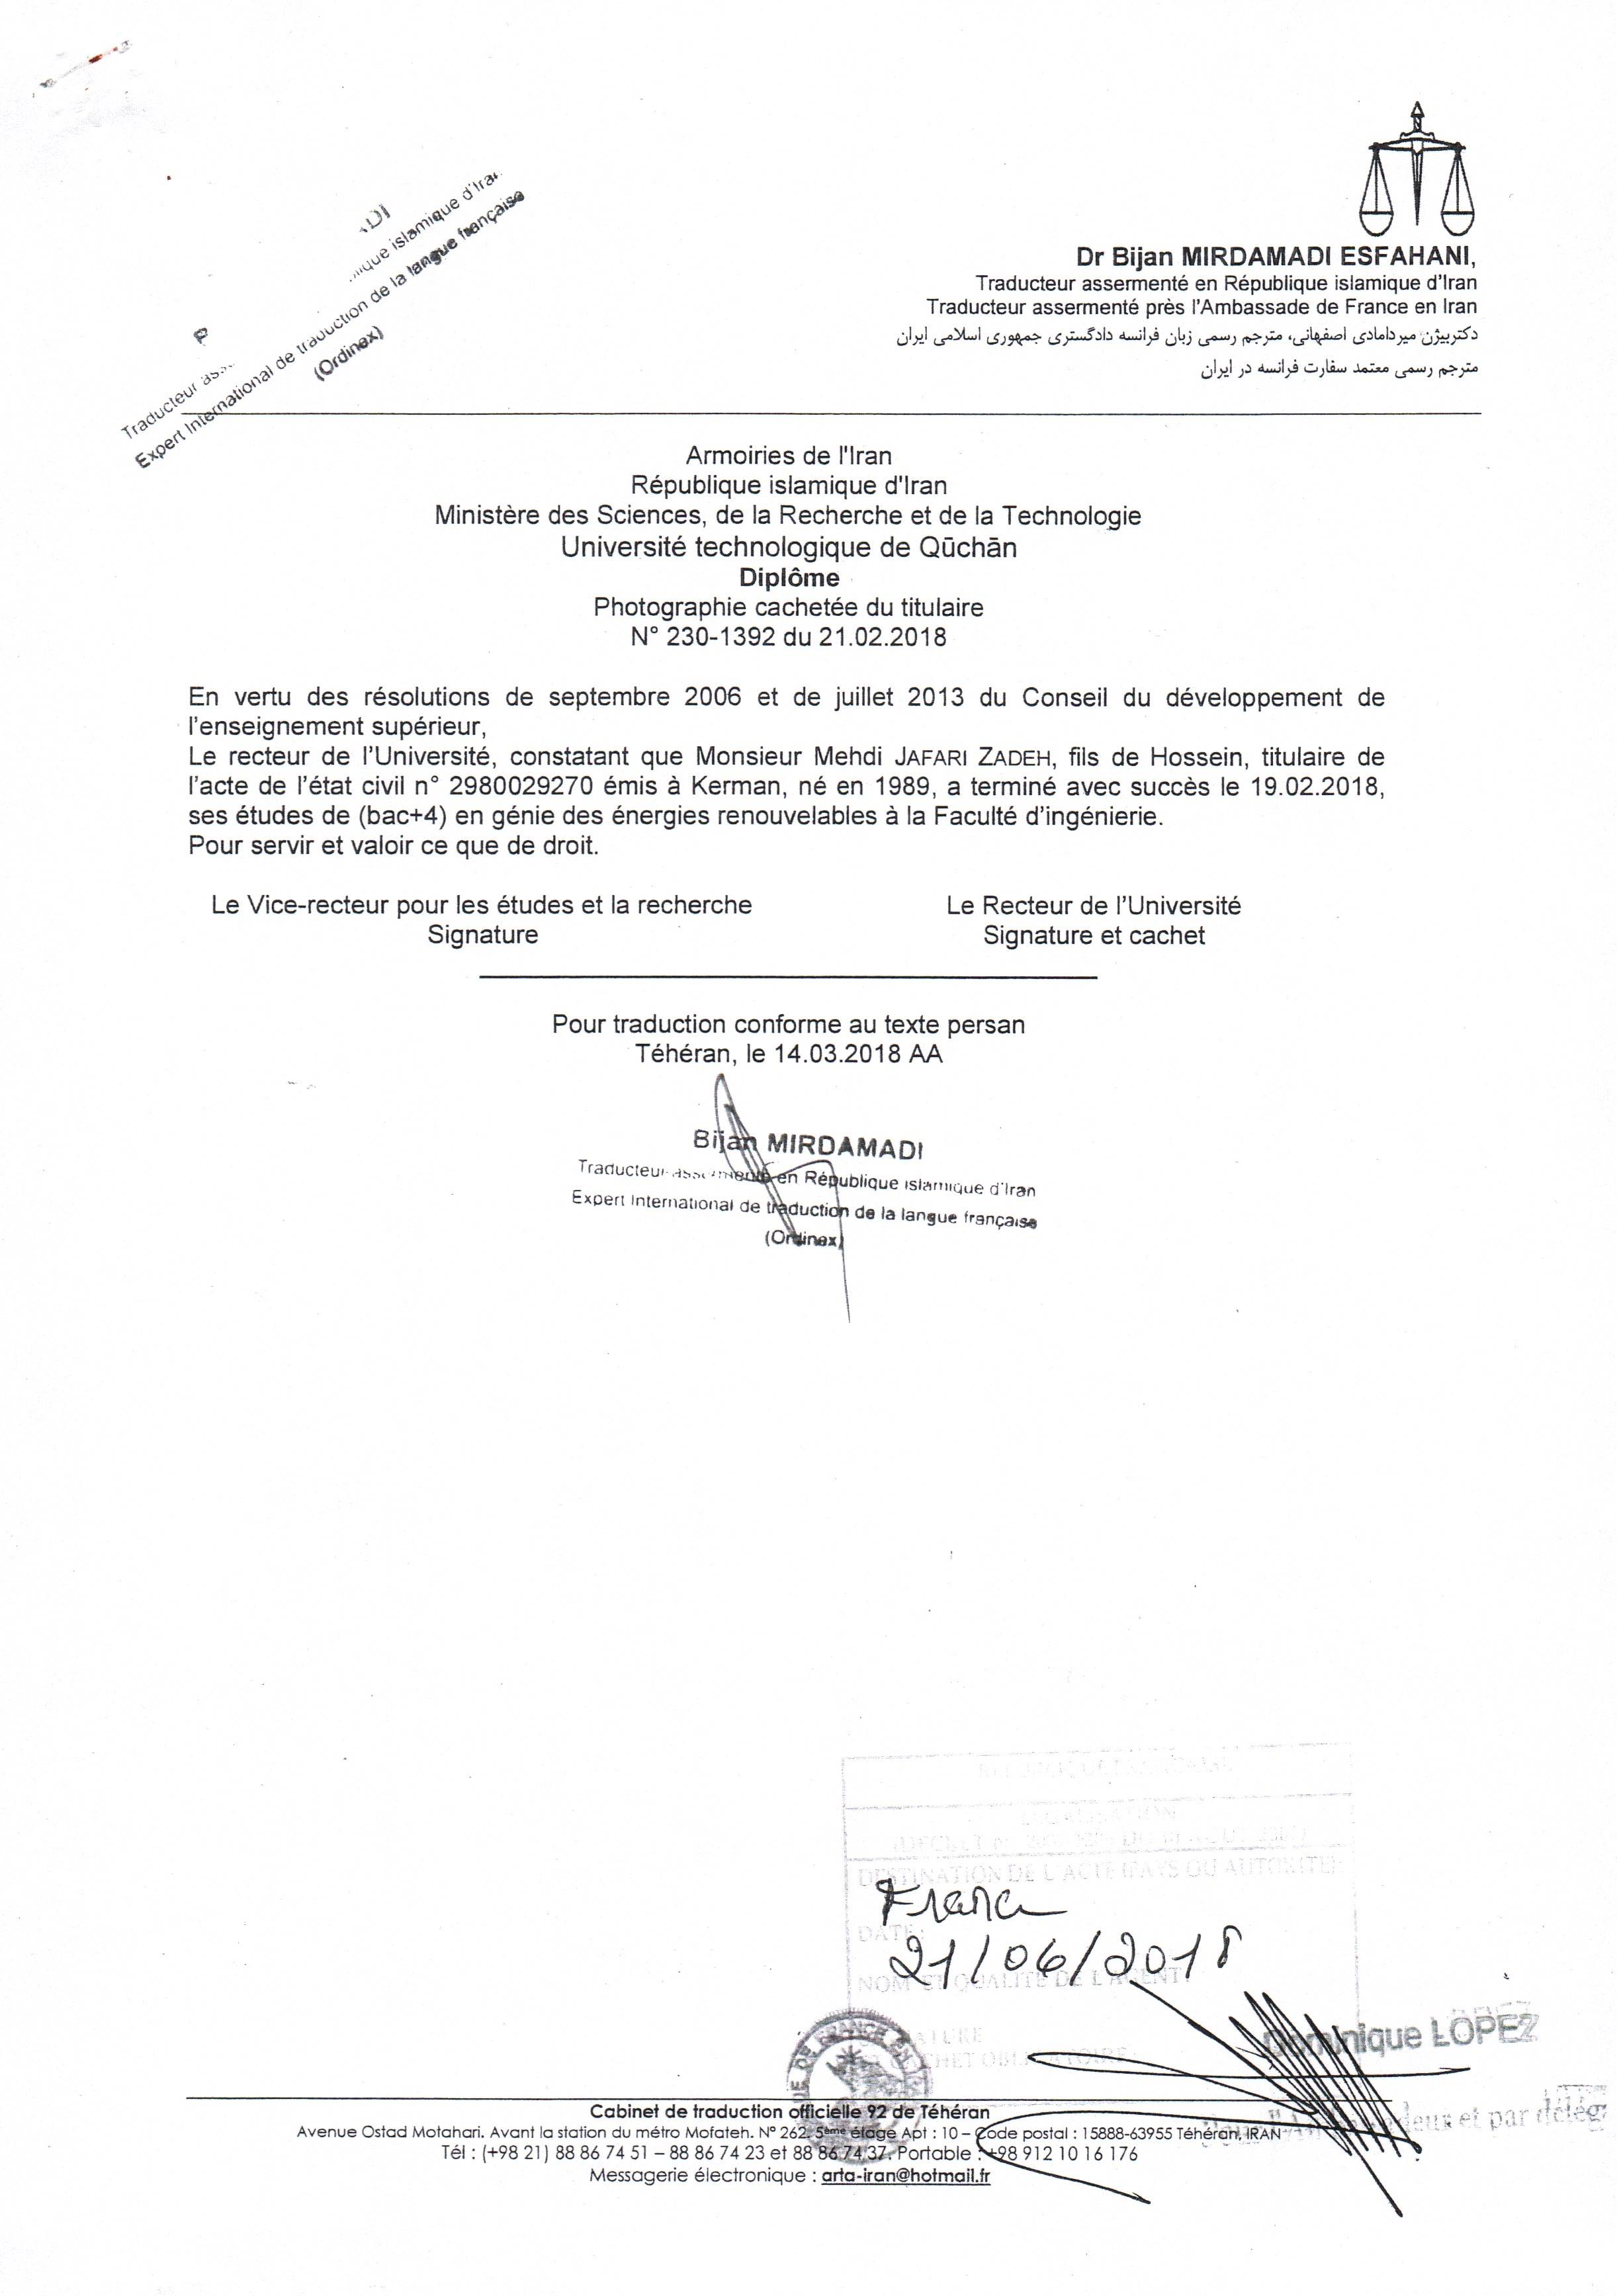
\includegraphics[width=\textwidth,height=\textheight,keepaspectratio]{../Document/Education/Renewable Energy Engineering/21-02-2018 diplôme - Génie énergétique.jpg}
        \footnotesize
         \href{https://github.com/jafarizadeh/CV---lettre/tree/079f60796b41475881d7ba4a70abc3254d3dd466/Document/Education/Renewable%20Energy%20Engineering}{Veuillez cliquer ici pour accéder au document sur GitHub.}.
    \end{center}
    
    \begin{center}
        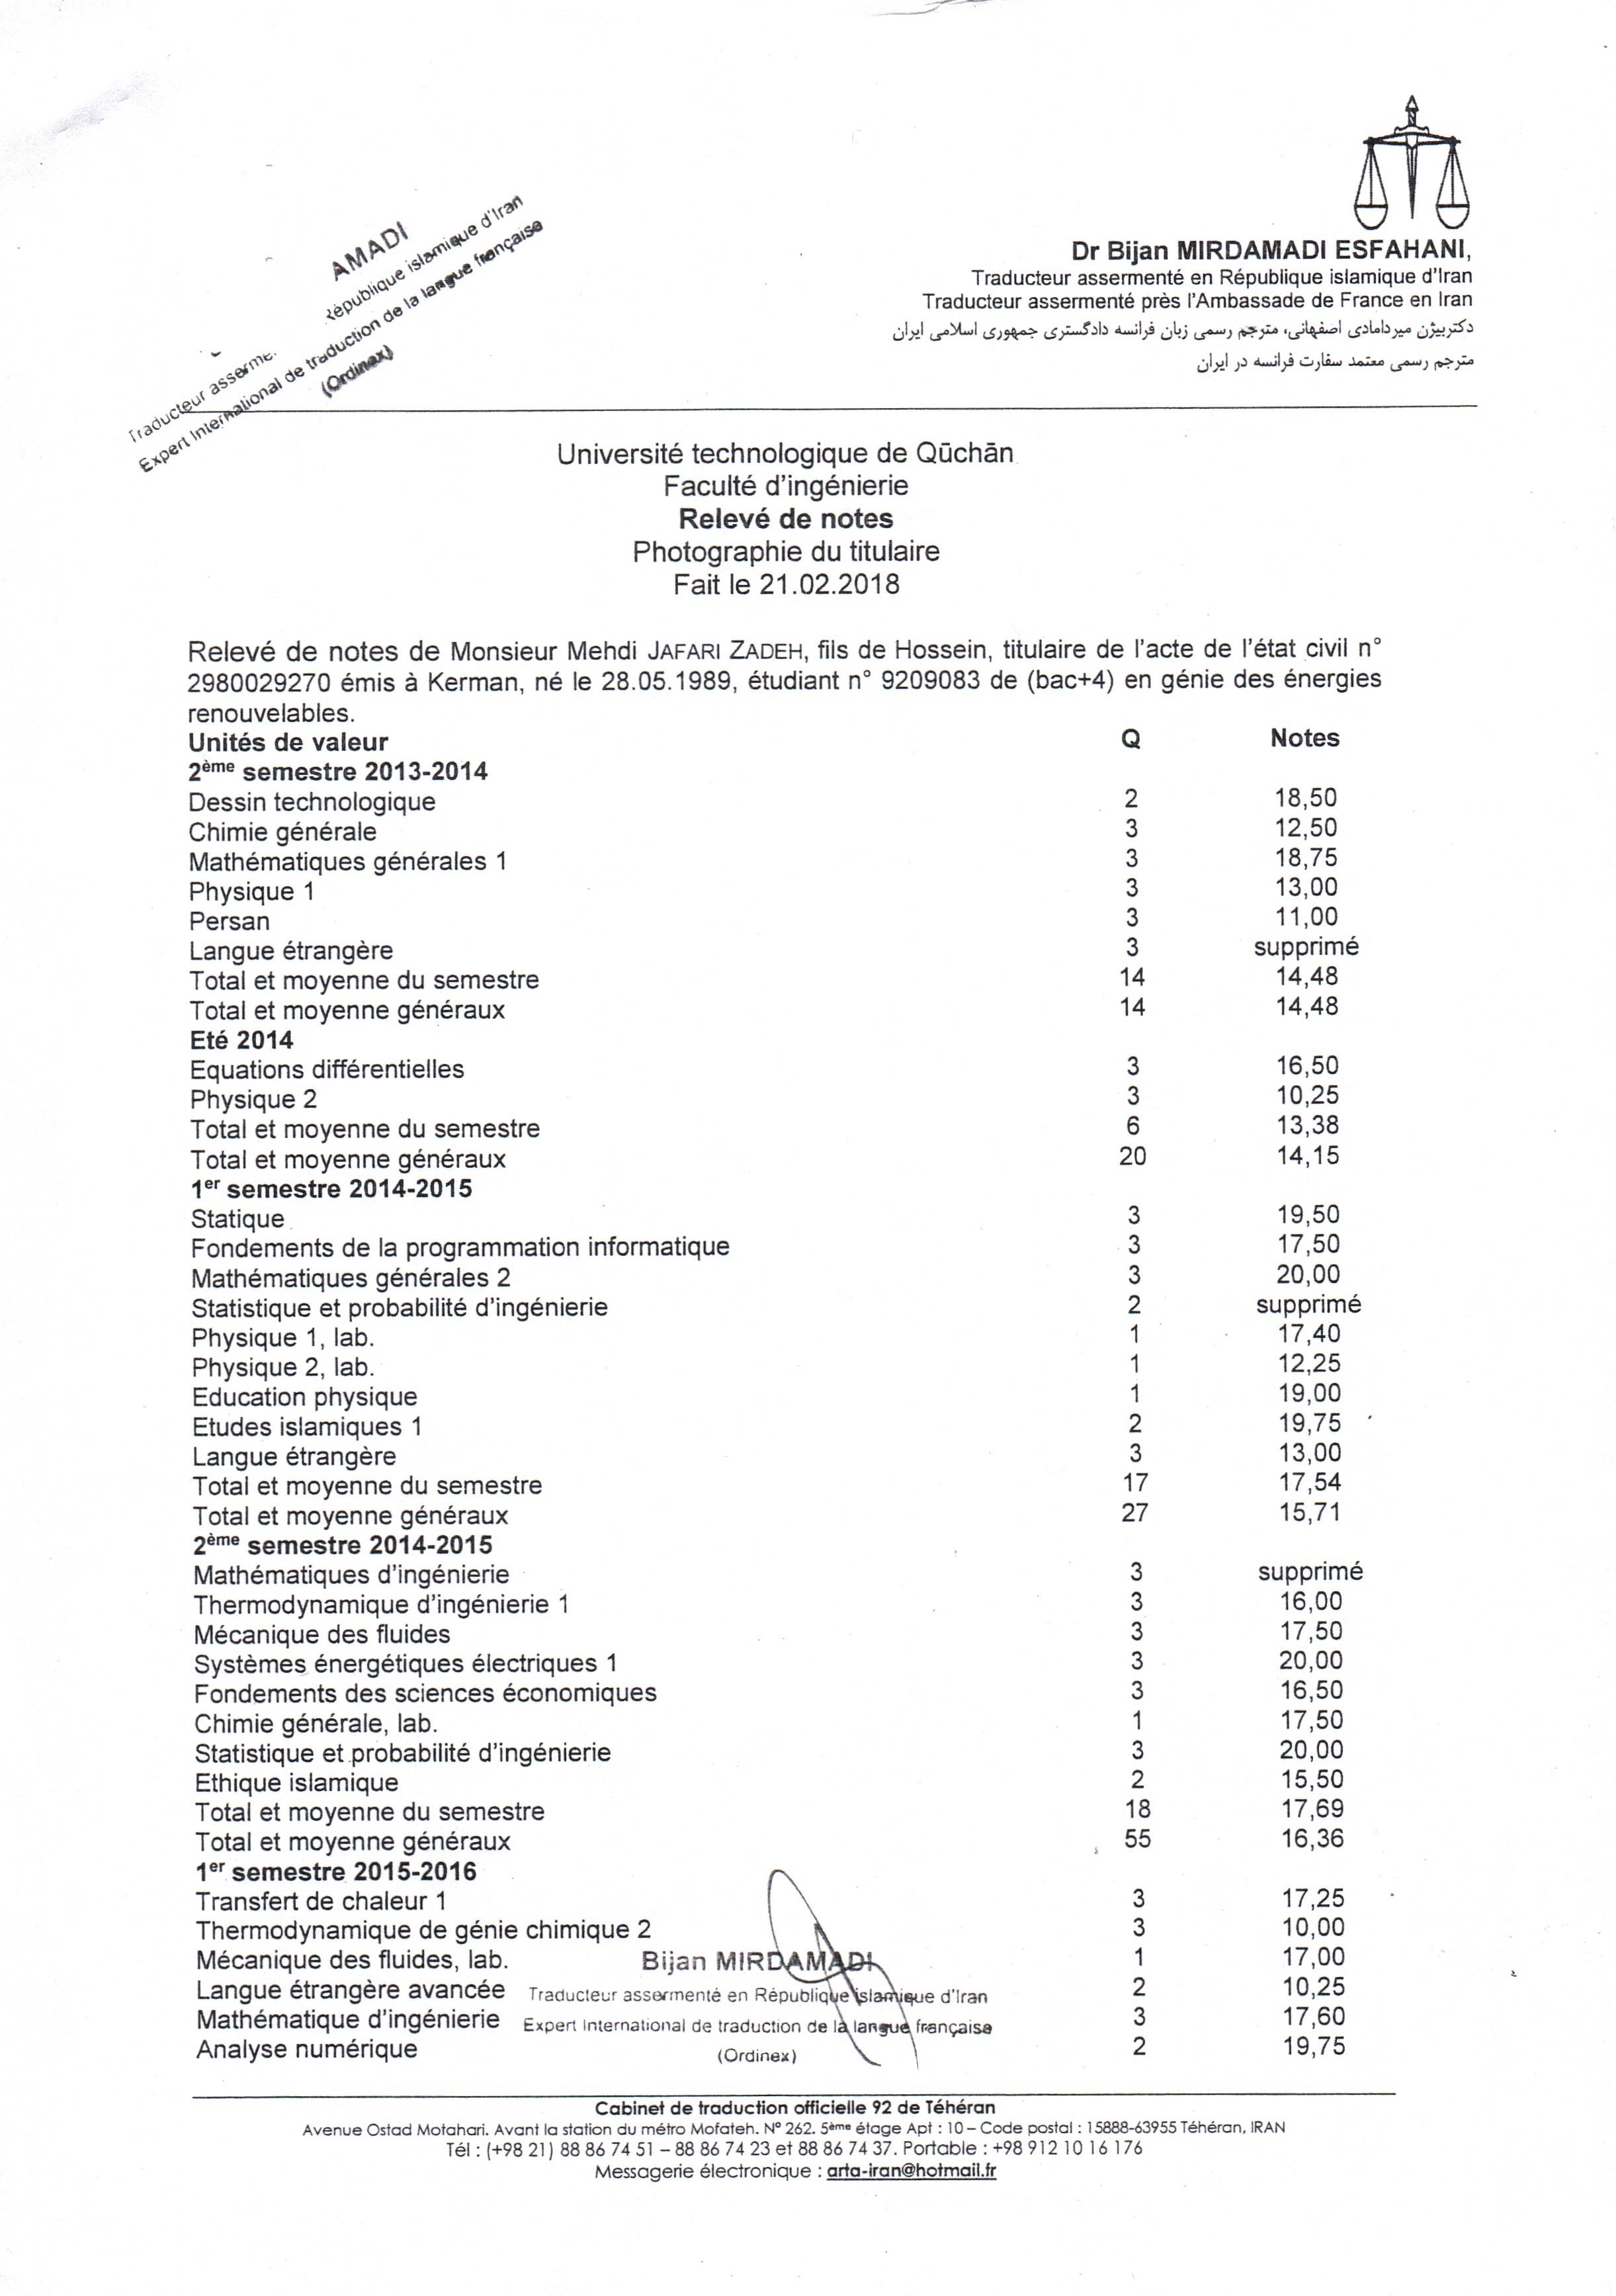
\includegraphics[width=\textwidth,height=\textheight,keepaspectratio]{../Document/Education/Renewable Energy Engineering/21-02-2018 releve de notes - Génie énergétique - P01.jpg}
        \small\vspace{0.5em} 
        \href{https://github.com/jafarizadeh/CV---lettre/tree/079f60796b41475881d7ba4a70abc3254d3dd466/Document/Education/Renewable%20Energy%20Engineering}{Veuillez cliquer ici pour accéder au document sur GitHub}.
    \end{center}

    \begin{center}
        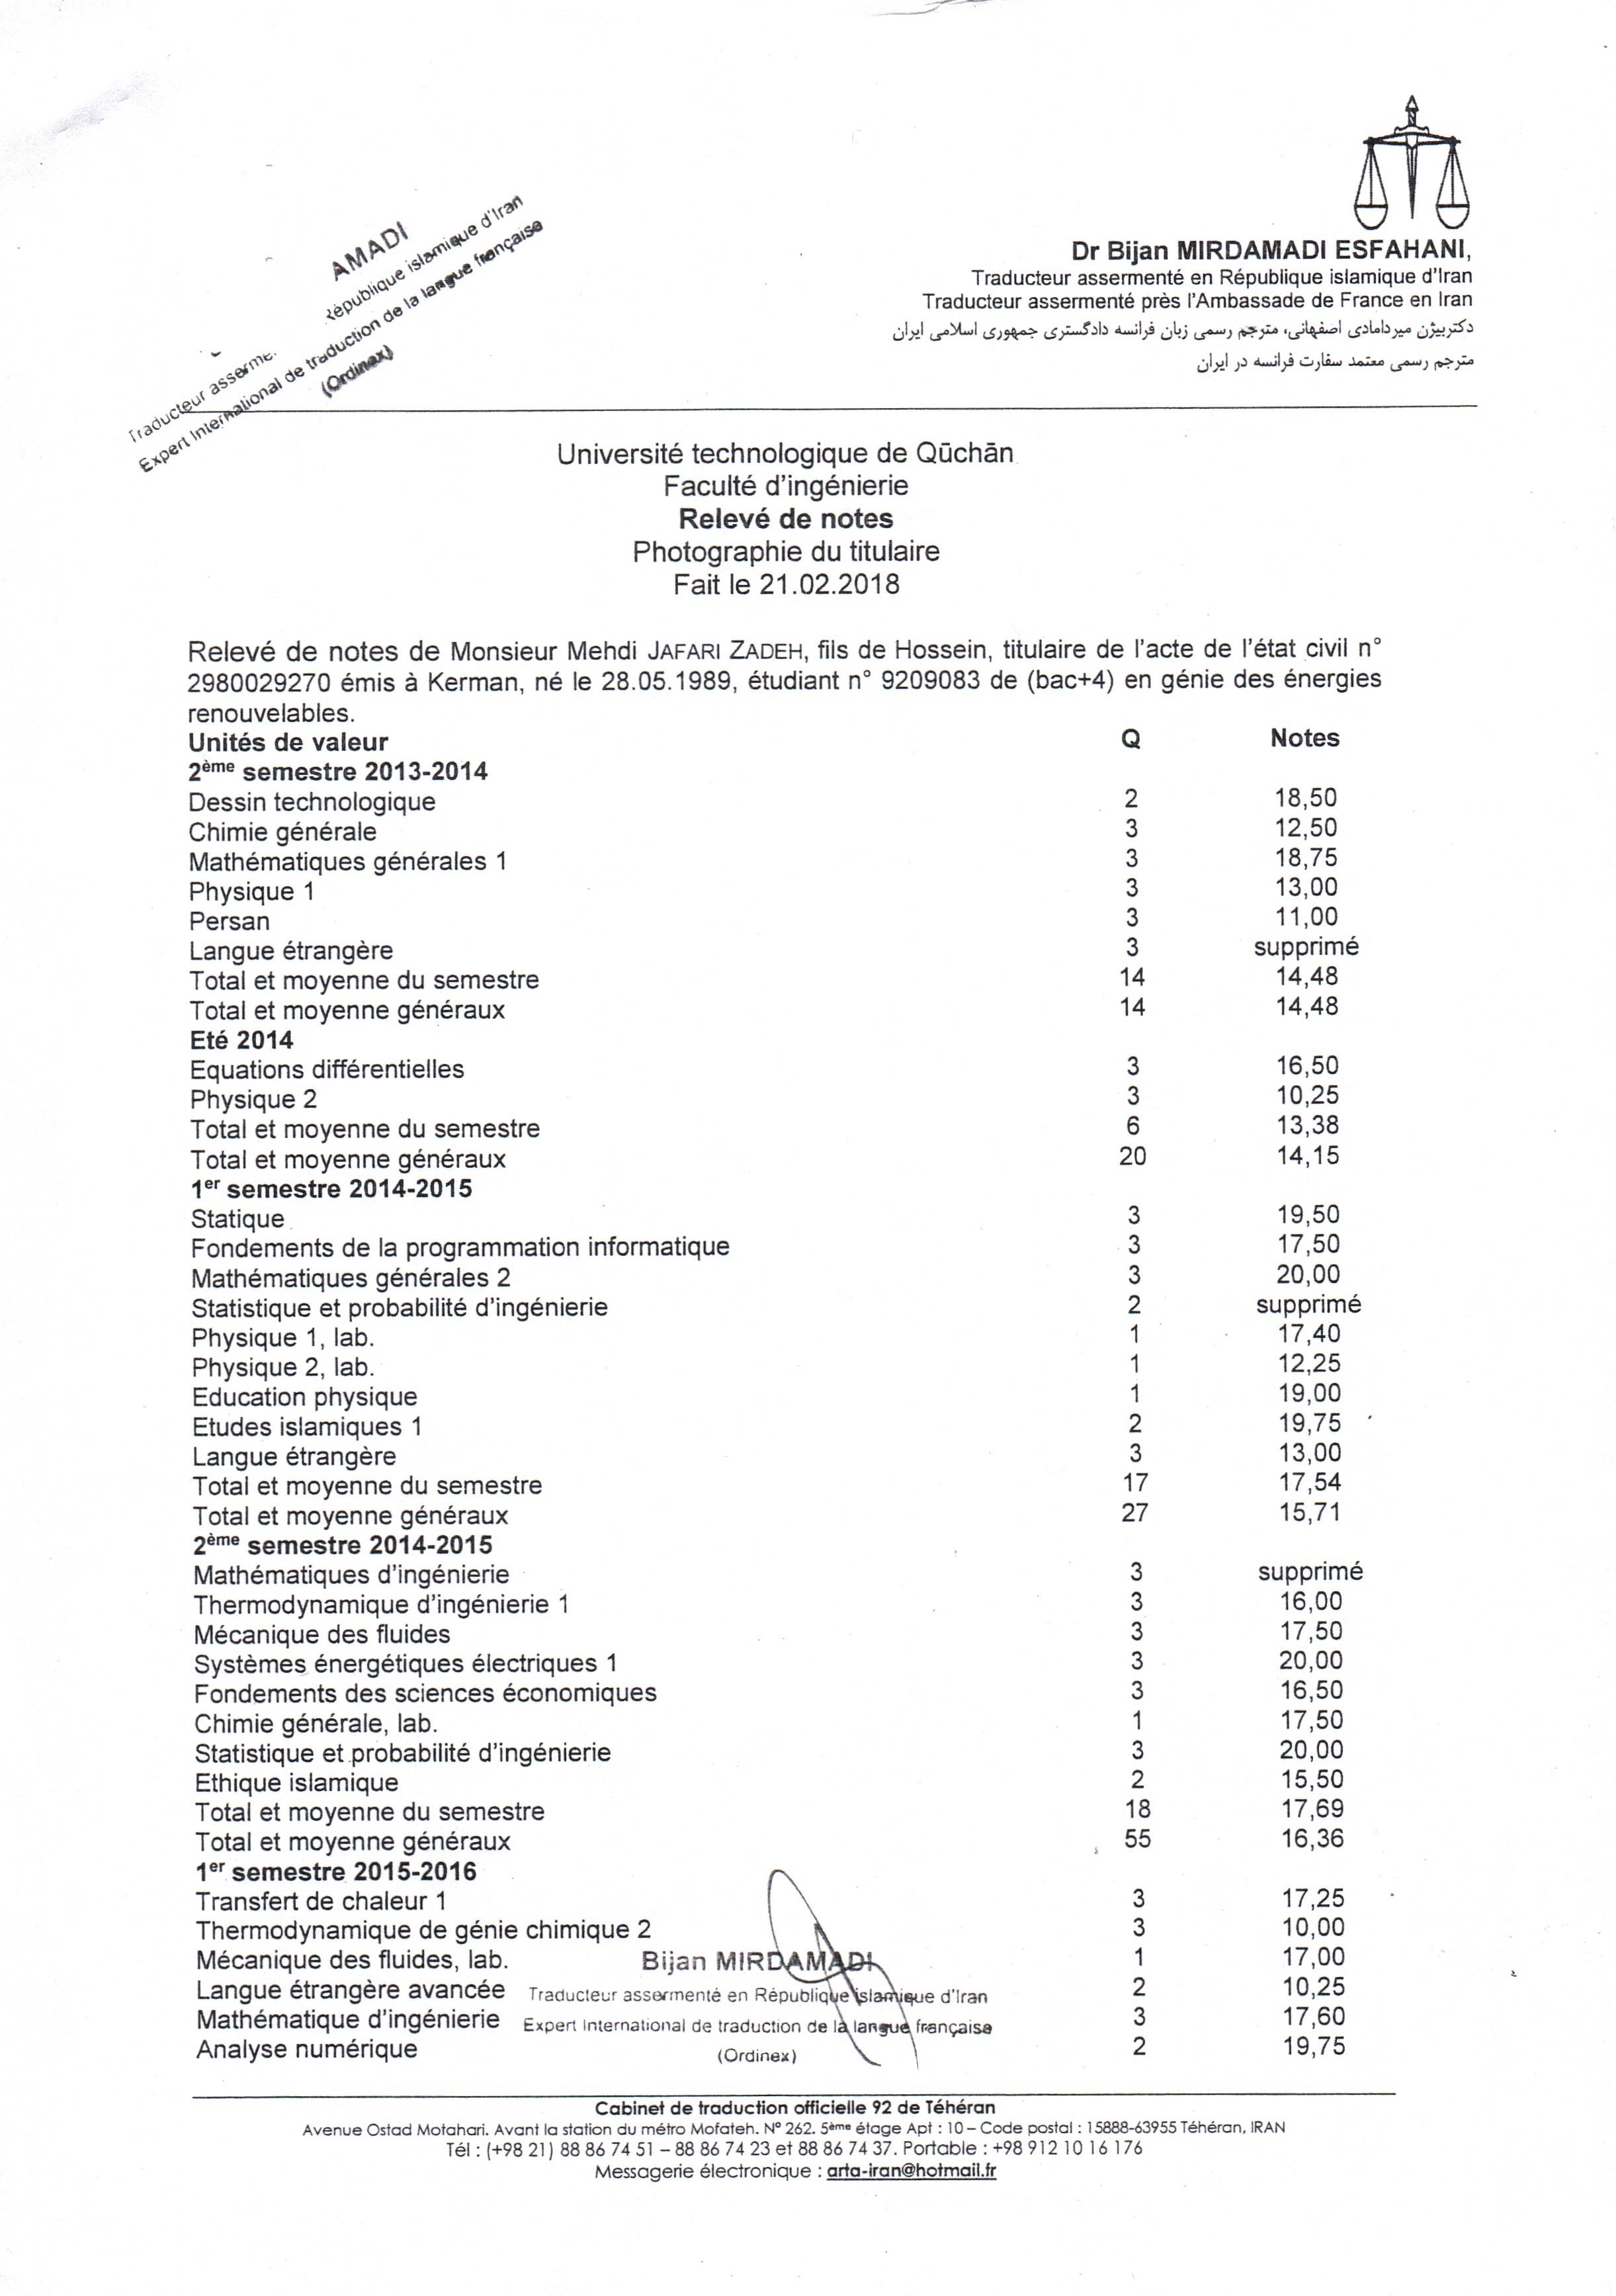
\includegraphics[width=\textwidth,height=\textheight,keepaspectratio]{../Document/Education/Renewable Energy Engineering/21-02-2018 releve de notes - Génie énergétique - P01.jpg}
        \footnotesize
         \href{https://github.com/jafarizadeh/CV---lettre/tree/079f60796b41475881d7ba4a70abc3254d3dd466/Document/Education/Renewable%20Energy%20Engineering}{Veuillez cliquer ici pour accéder au document sur GitHub}.
    \end{center}
    
\newpage

 
    \subsection{Comptabilité}
    
    \par\textbf{Informations supplémentaires:} J'ai obtenu un Brevet de Technicien Supérieur (BTS) en Comptabilité en 2010 à l'Université Azad de Kerman. Ce programme m'a permis de développer une solide expertise en gestion financière, en analyse des états financiers et en comptabilité analytique. Ces compétences ont été renforcées par des cours pratiques et des stages qui m'ont préparé à travailler efficacement dans divers environnements comptables et financiers. Grâce à cette formation, j'ai acquis une compréhension approfondie des principes comptables et fiscaux, ainsi que des compétences techniques essentielles pour gérer les opérations financières d'une entreprise.
    \newline
    \newline
    \textit {Note: Des images de la traduction Française de ce document sont incluses dans les pages suivantes.}

        \begin{center}
            \includegraphics[width=\textwidth,height=\textheight,keepaspectratio]{../Document/Education/Accounting/31-09-2011 diplôme - Comptabilite.jpg}
            \footnotesize
            \href{https://github.com/jafarizadeh/CV---lettre/tree/079f60796b41475881d7ba4a70abc3254d3dd466/Document/Education/Accounting}{Veuillez cliquer ici pour accéder au document sur GitHub}.
        \end{center}

        \begin{center}
            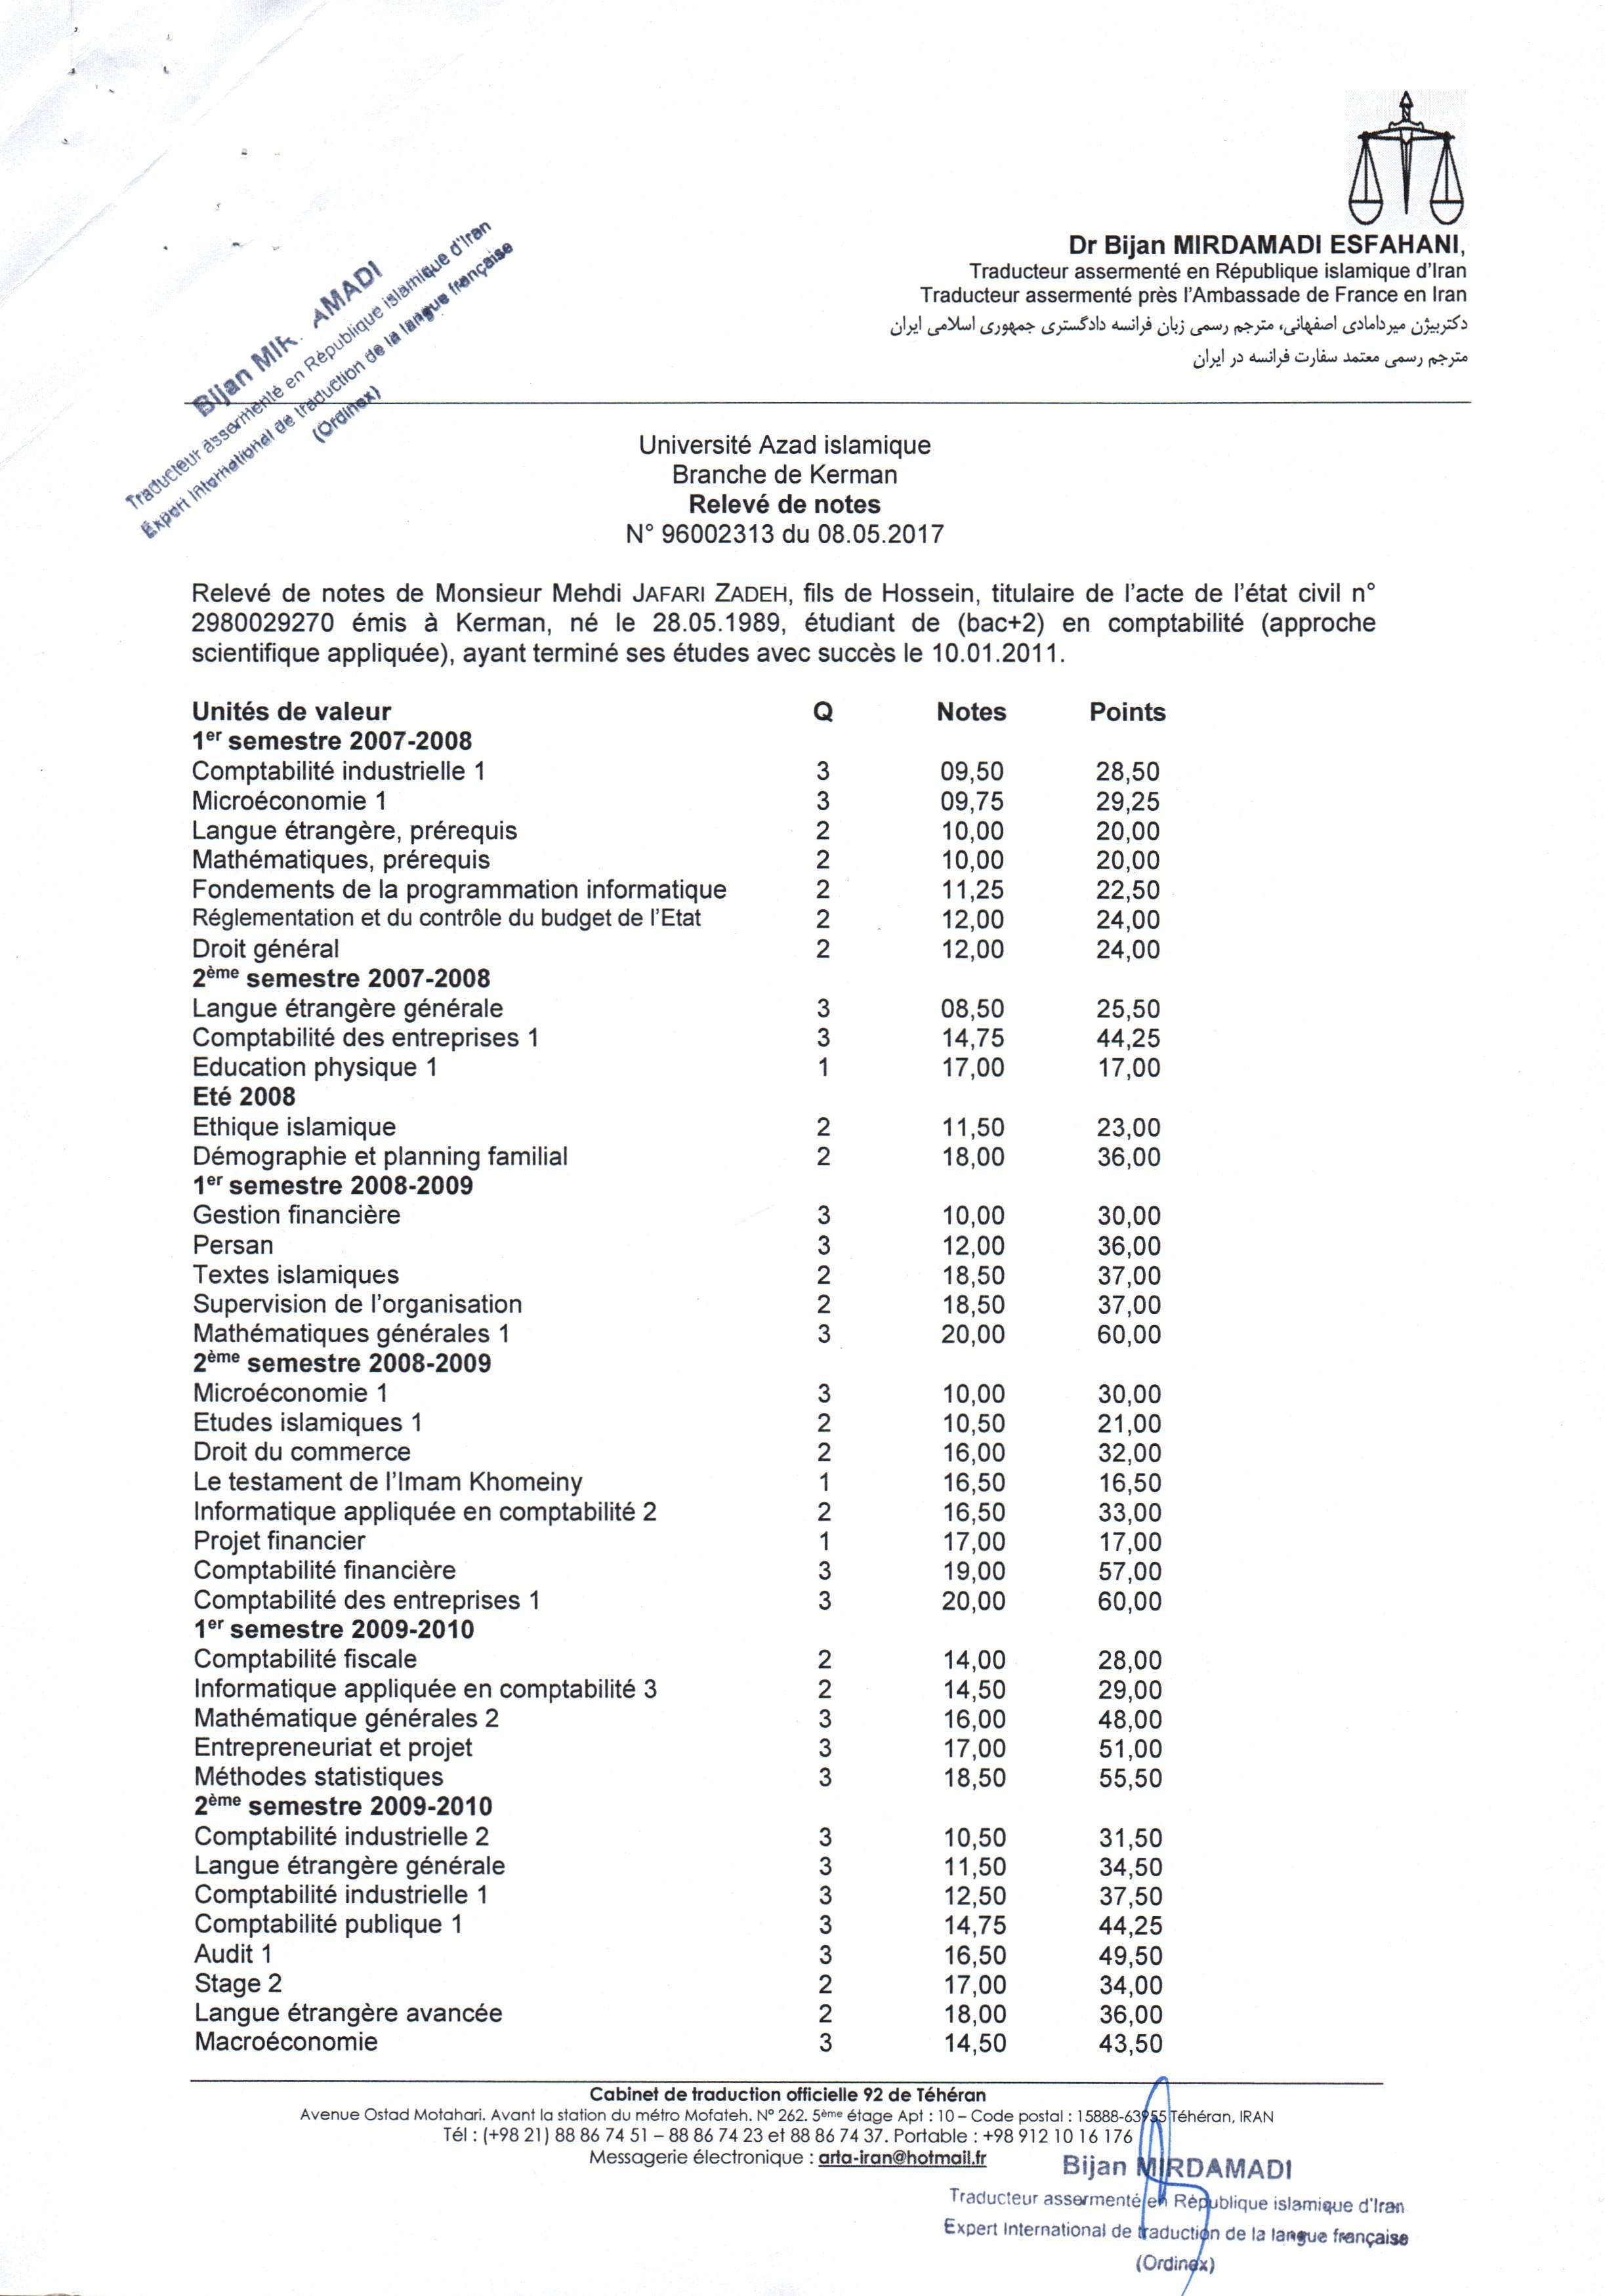
\includegraphics[width=\textwidth,height=\textheight,keepaspectratio]{../Document/Education/Accounting/08-05-2017 releve de notes - Comptabilite - P01.jpg}
            \footnotesize
            \href{https://github.com/jafarizadeh/CV---lettre/tree/079f60796b41475881d7ba4a70abc3254d3dd466/Document/Education/Accounting}{Veuillez cliquer ici pour accéder au document sur GitHub}.
        \end{center}

        \begin{center}
            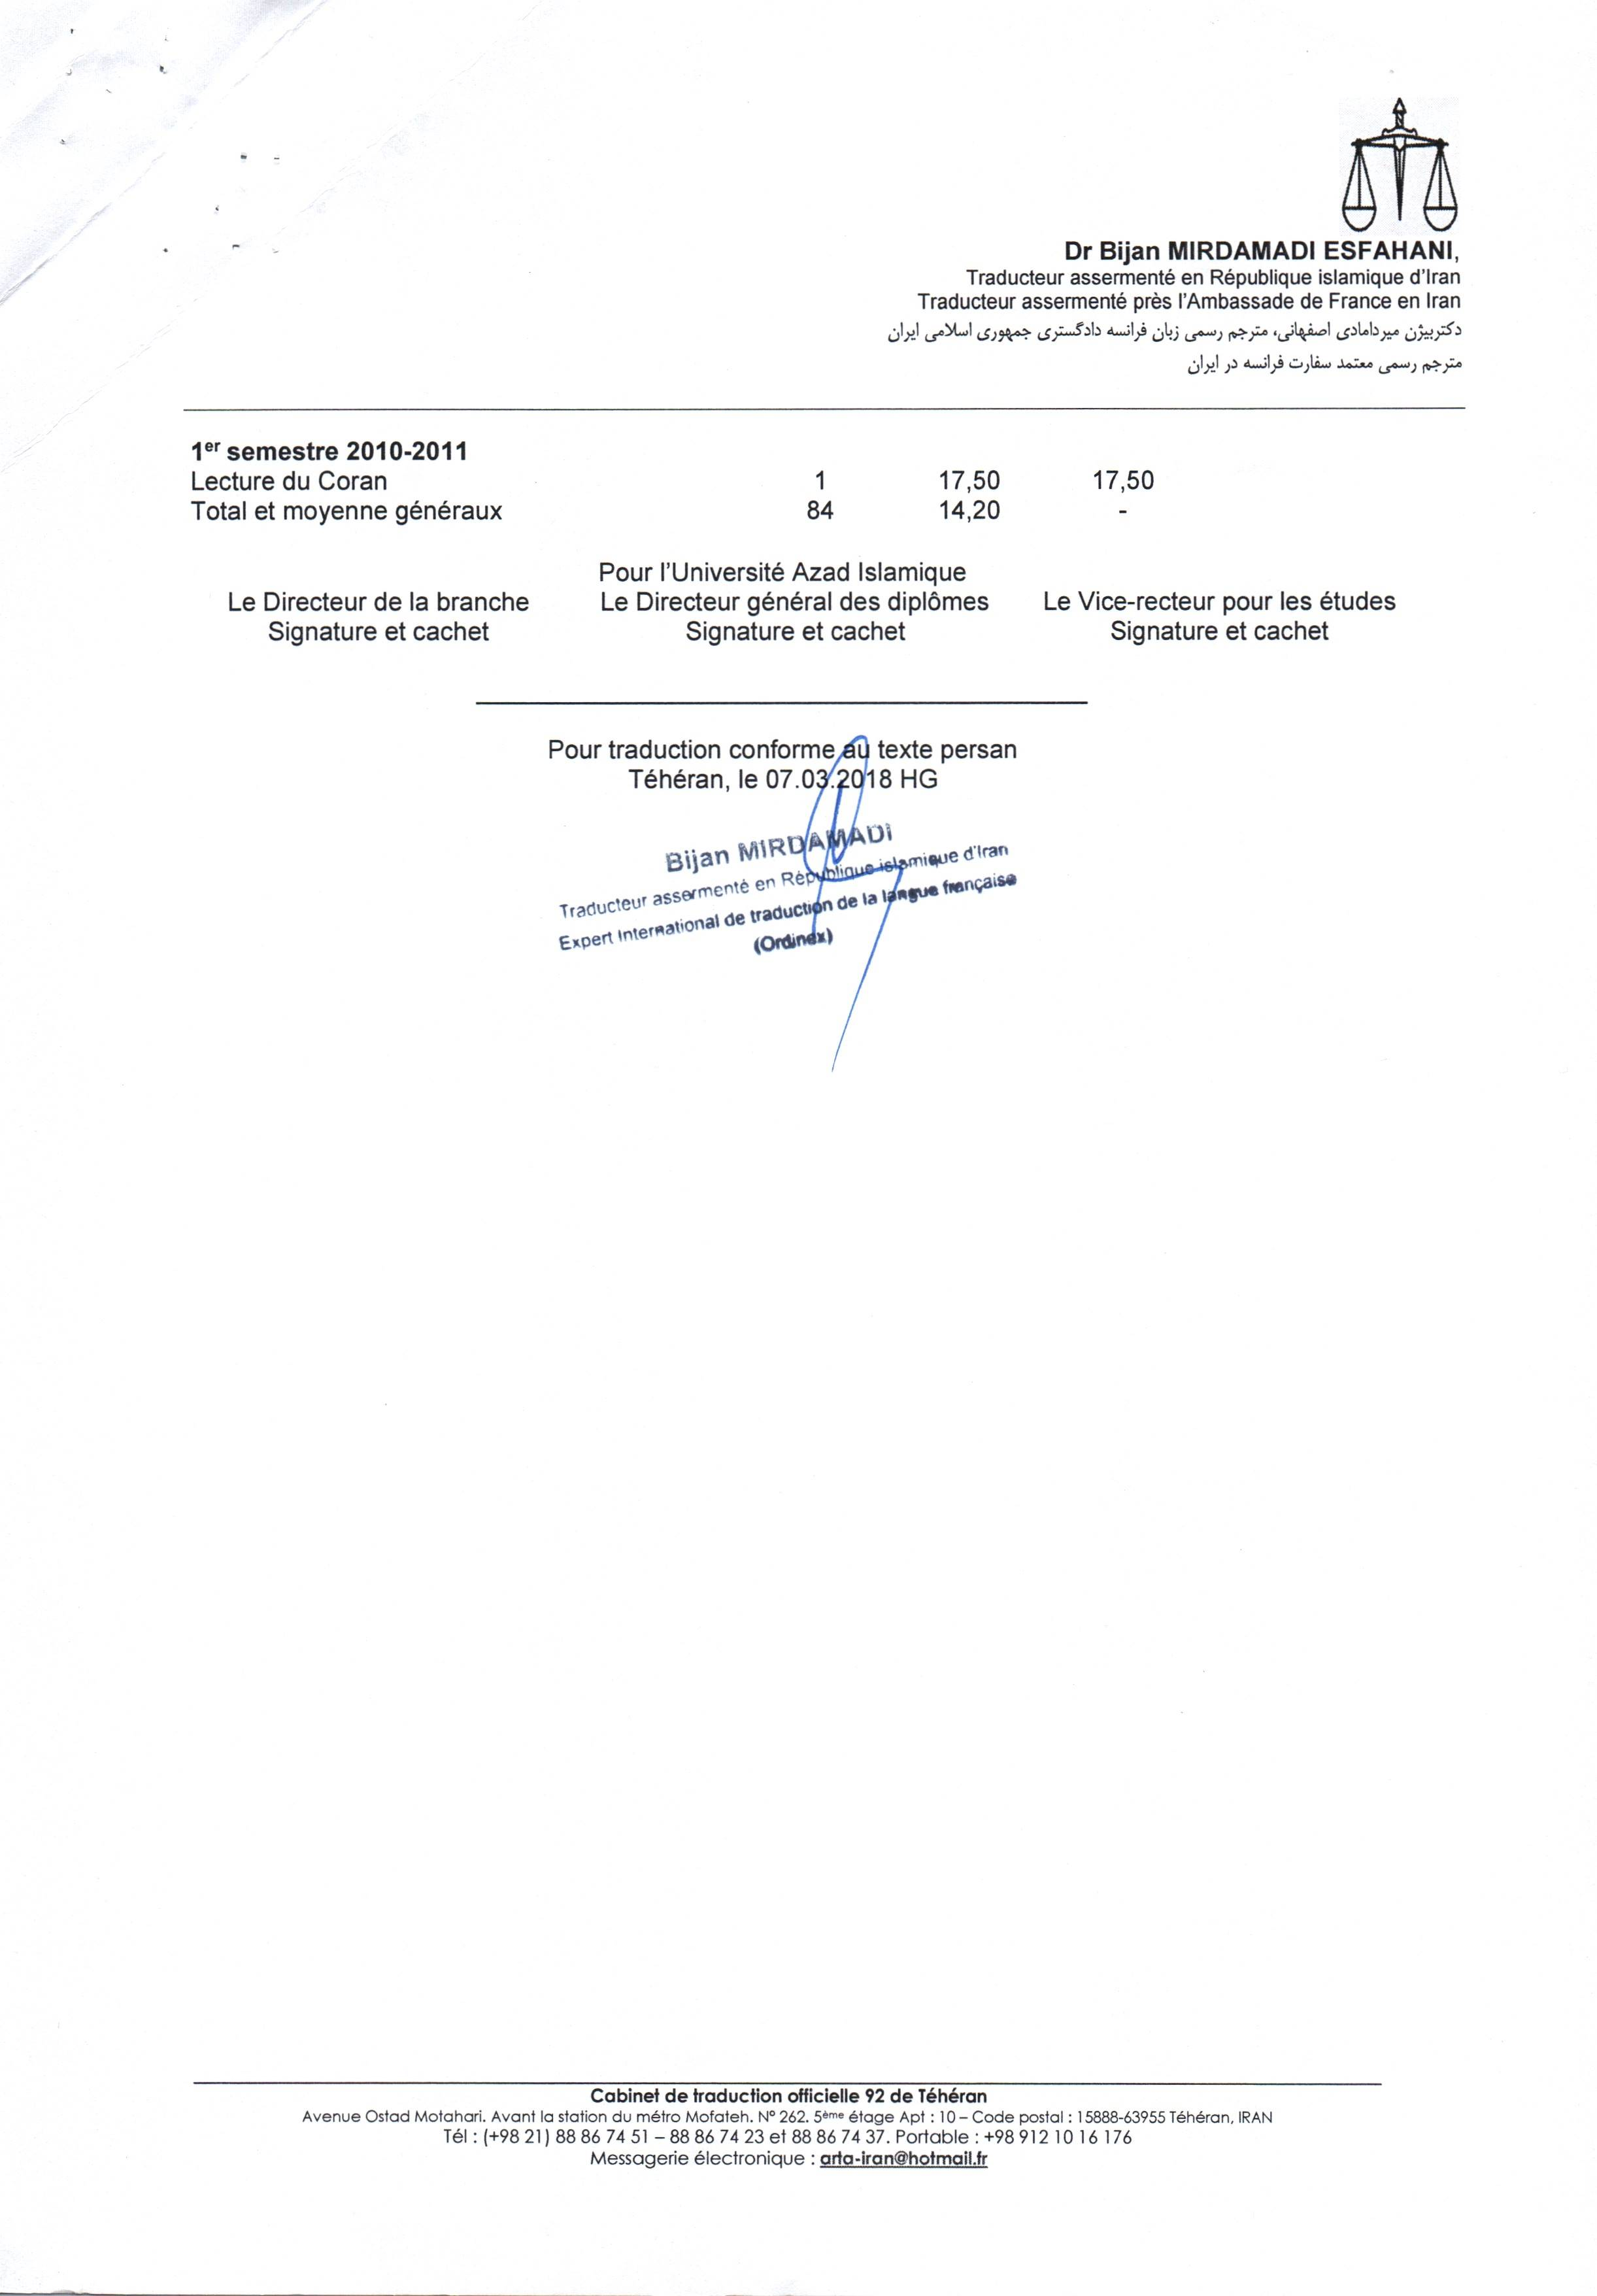
\includegraphics[width=\textwidth,height=\textheight,keepaspectratio]{../Document/Education/Accounting/08-05-2017 releve de notes - Comptabilite - P02.jpg}
            \footnotesize
             \href{https://github.com/jafarizadeh/CV---lettre/tree/079f60796b41475881d7ba4a70abc3254d3dd466/Document/Education/Accounting}{Veuillez cliquer ici pour accéder au document sur GitHub}.
        \end{center}

    \newpage

   
% =========================================================
% ============== Expérience Professionnelle ===============
% =========================================================


\section{Expérience Professionnelle}

    % 3.1 Teaching assistant
    \subsection{Assistant d'Enseignement}

    Pendant mes études en Ingénierie de l'Énergie, j'ai eu l'opportunité de travailler comme Assistant d'Enseignement pour les cours de Mathématiques et de Conversion d'Énergie. Ma solide maîtrise des mathématiques et des calculs d'ingénierie m'a permis de dispenser des cours, de guider les étudiants et d'assister efficacement dans les projets liés aux cours. Gérer l'environnement de la classe et répondre aux besoins divers des étudiants figuraient parmi les principaux défis auxquels j'ai été confronté. Cependant, en appliquant des stratégies de communication et de gestion efficaces, j'ai réussi à surmonter ces défis, gagnant ainsi le respect et la satisfaction tant des étudiants que des professeurs expérimentés.
    \newline
    \newline
    \textit {Note: Une image de la traduction Française de ce document est incluse dans les pages suivantes.}
    \newline
    \newline

    \newpage

        \begin{center}
            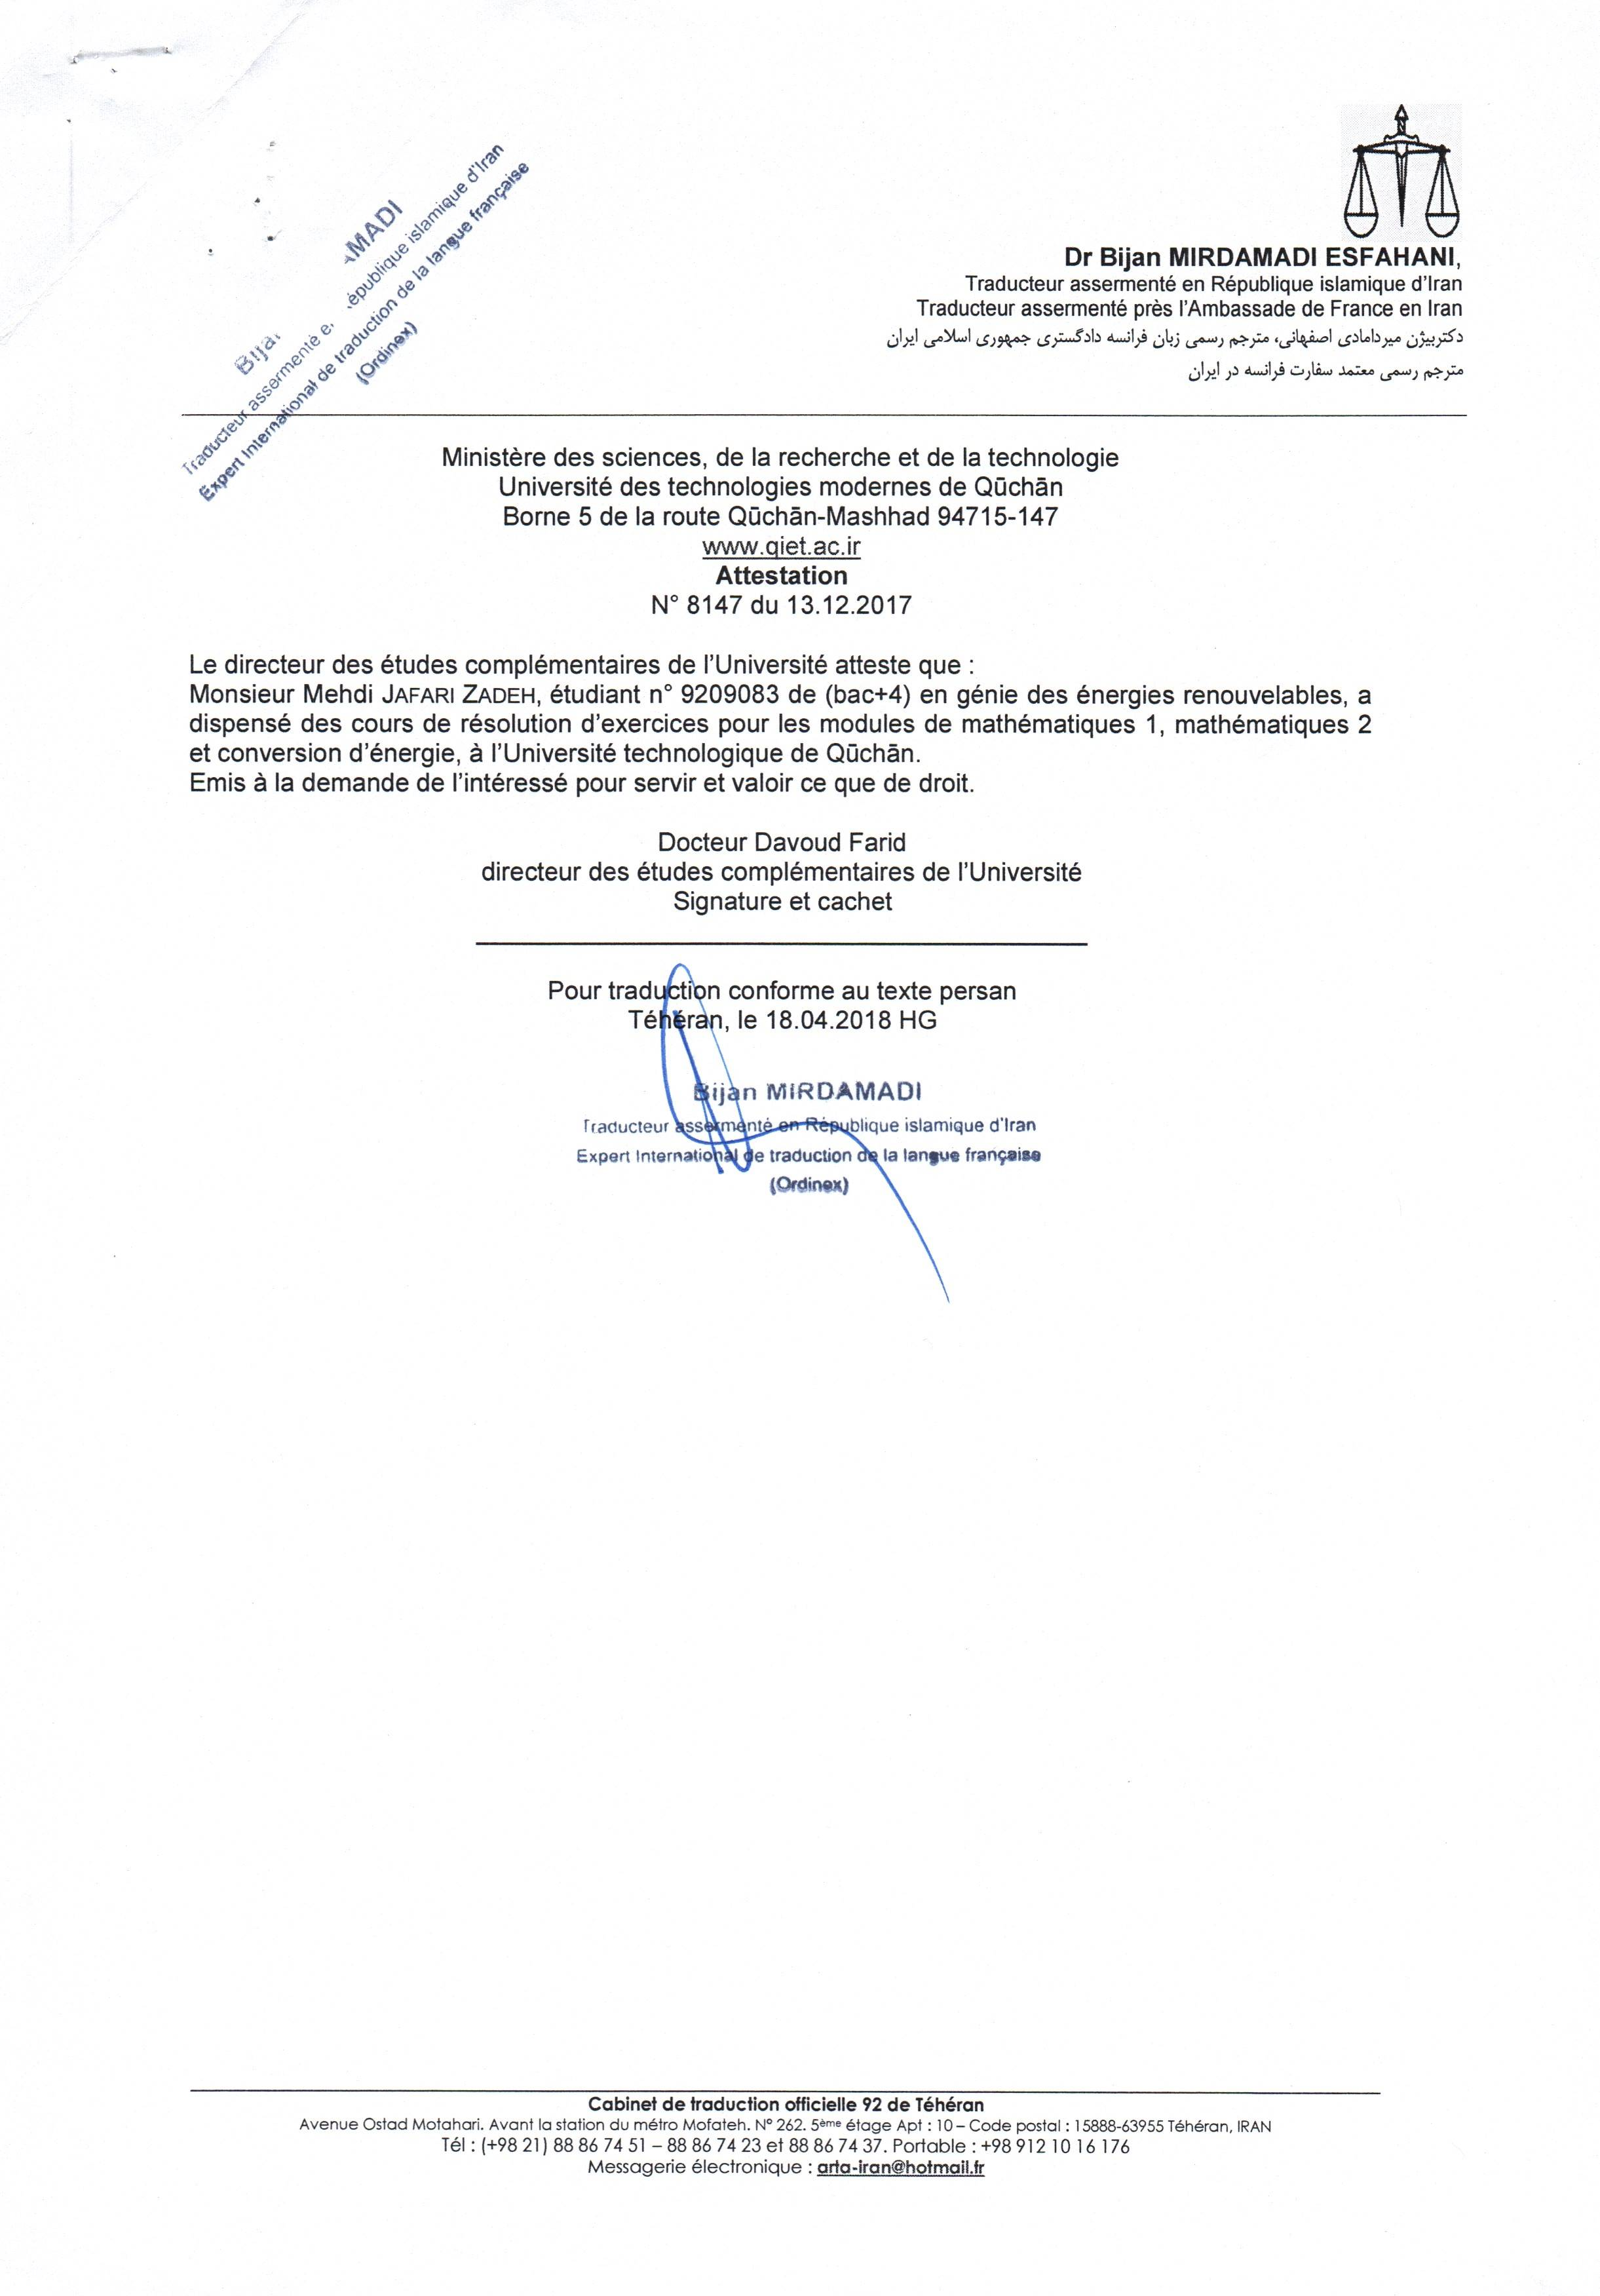
\includegraphics[width=\textwidth,height=\textheight,keepaspectratio]{../Document/Work Experience/Teaching Assistant/13-12-2017 attestation.jpg}
            \footnotesize
             \href{https://github.com/jafarizadeh/CV---lettre/tree/079f60796b41475881d7ba4a70abc3254d3dd466/Document/Work%20Experience/Teaching%20Assistant}{Veuillez cliquer ici pour accéder au document sur GitHub}.
        \end{center}
    
    % 3.2 Founder of the Energy Engineering Association
    \subsection{Fondateur de l'Association d'Ingénierie de l'Énergie}

    \par
    En mai 2015, j'ai cofondé l'Association d'Ingénierie de l'Énergie à l'Université de Technologie de Quchan avec un groupe de pairs passionnés. Notre objectif principal était de fournir une formation complémentaire et une expérience pratique aux étudiants intéressés par l'ingénierie énergétique. Cette initiative comprenait l'organisation d'ateliers avec des professeurs expérimentés, l'accueil de compétitions scientifiques et la coordination de projets de groupe qui amélioraient les compétences techniques des étudiants au-delà du programme standard.

    Au cours de trois années, l'association a réussi à organiser trois compétitions scientifiques, cinq cours de formation spécialisée en logiciels, et un cours d'entrepreneuriat destiné à préparer les étudiants aux défis professionnels après l'obtention de leur diplôme. Ces activités ont non seulement favorisé un environnement d'apprentissage collaboratif, mais ont également contribué de manière significative à la croissance professionnelle et à la préparation des étudiants impliqués.
    \newline
    \newline
    \textit {Note: Une image de la traduction Française de ce document est incluse dans les pages suivantes.}
    \newline
    \newline

    \newpage

        \begin{center}
            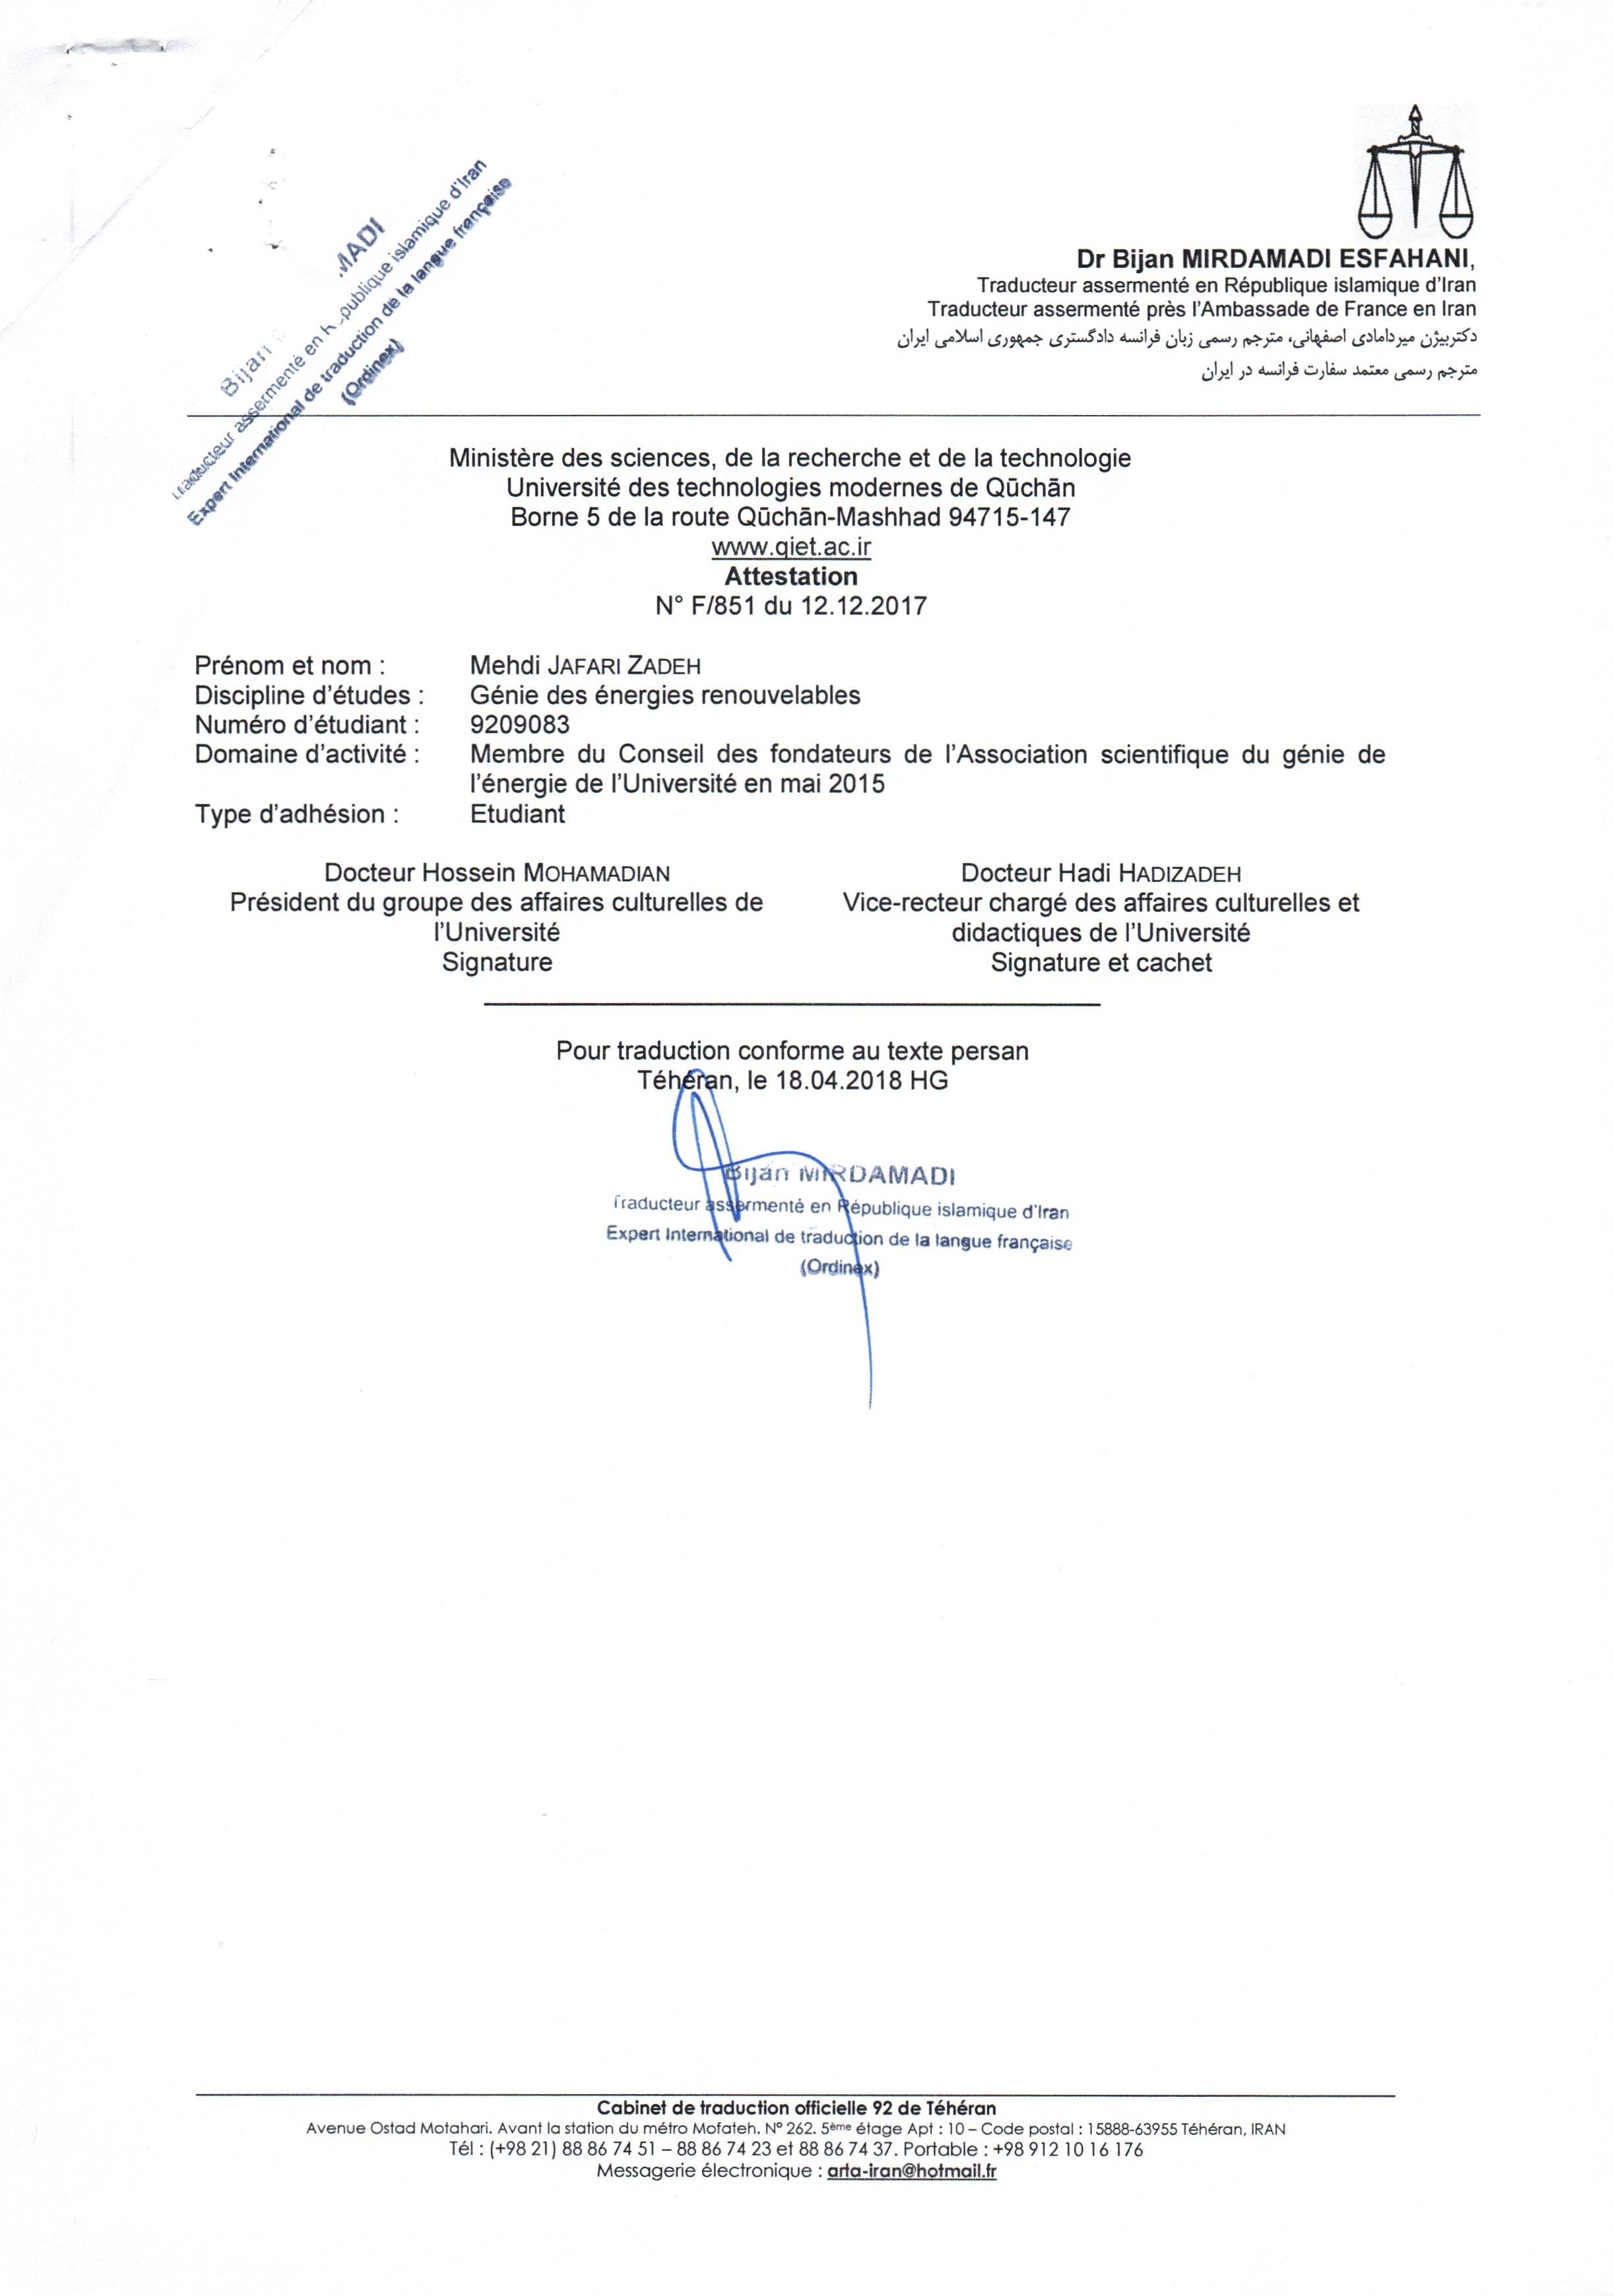
\includegraphics[width=\textwidth,height=\textheight,keepaspectratio]{../Document/Work Experience/Founder of the Energy Engineering Association/12-12-2017 attestation.jpg}
            \footnotesize
             \href{https://github.com/jafarizadeh/CV---lettre/tree/079f60796b41475881d7ba4a70abc3254d3dd466/Document/Work%20Experience/Founder%20of%20the%20Energy%20Engineering%20Association}{Veuillez cliquer ici pour accéder au document sur GitHub}.
        \end{center}

    % 3.3 Director of the Energy Engineering Association
    \subsection{Directeur de l'Association d'Ingénierie de l'Énergie}

    \par
    Élu par les responsables universitaires et les étudiants, j'ai occupé le poste de Directeur de l'Association d'Ingénierie de l'Énergie pendant cinq semestres consécutifs. Au cours de mon mandat, j'ai dirigé diverses initiatives visant à promouvoir les pratiques énergétiques durables au sein de la communauté universitaire. Mes compétences en leadership et en gestion ont été reconnues à plusieurs reprises par des certificats de reconnaissance du président de l'université. Mon rôle consistait à organiser des événements, gérer les budgets, et coordonner avec des parties prenantes externes pour faire avancer les objectifs de l'association.
    \newline
    \newline
    \textit {Note: Une image de la traduction Française de ce document est incluse dans les pages suivantes.}
    \newline
    \newline

    \newpage

        \begin{center}
            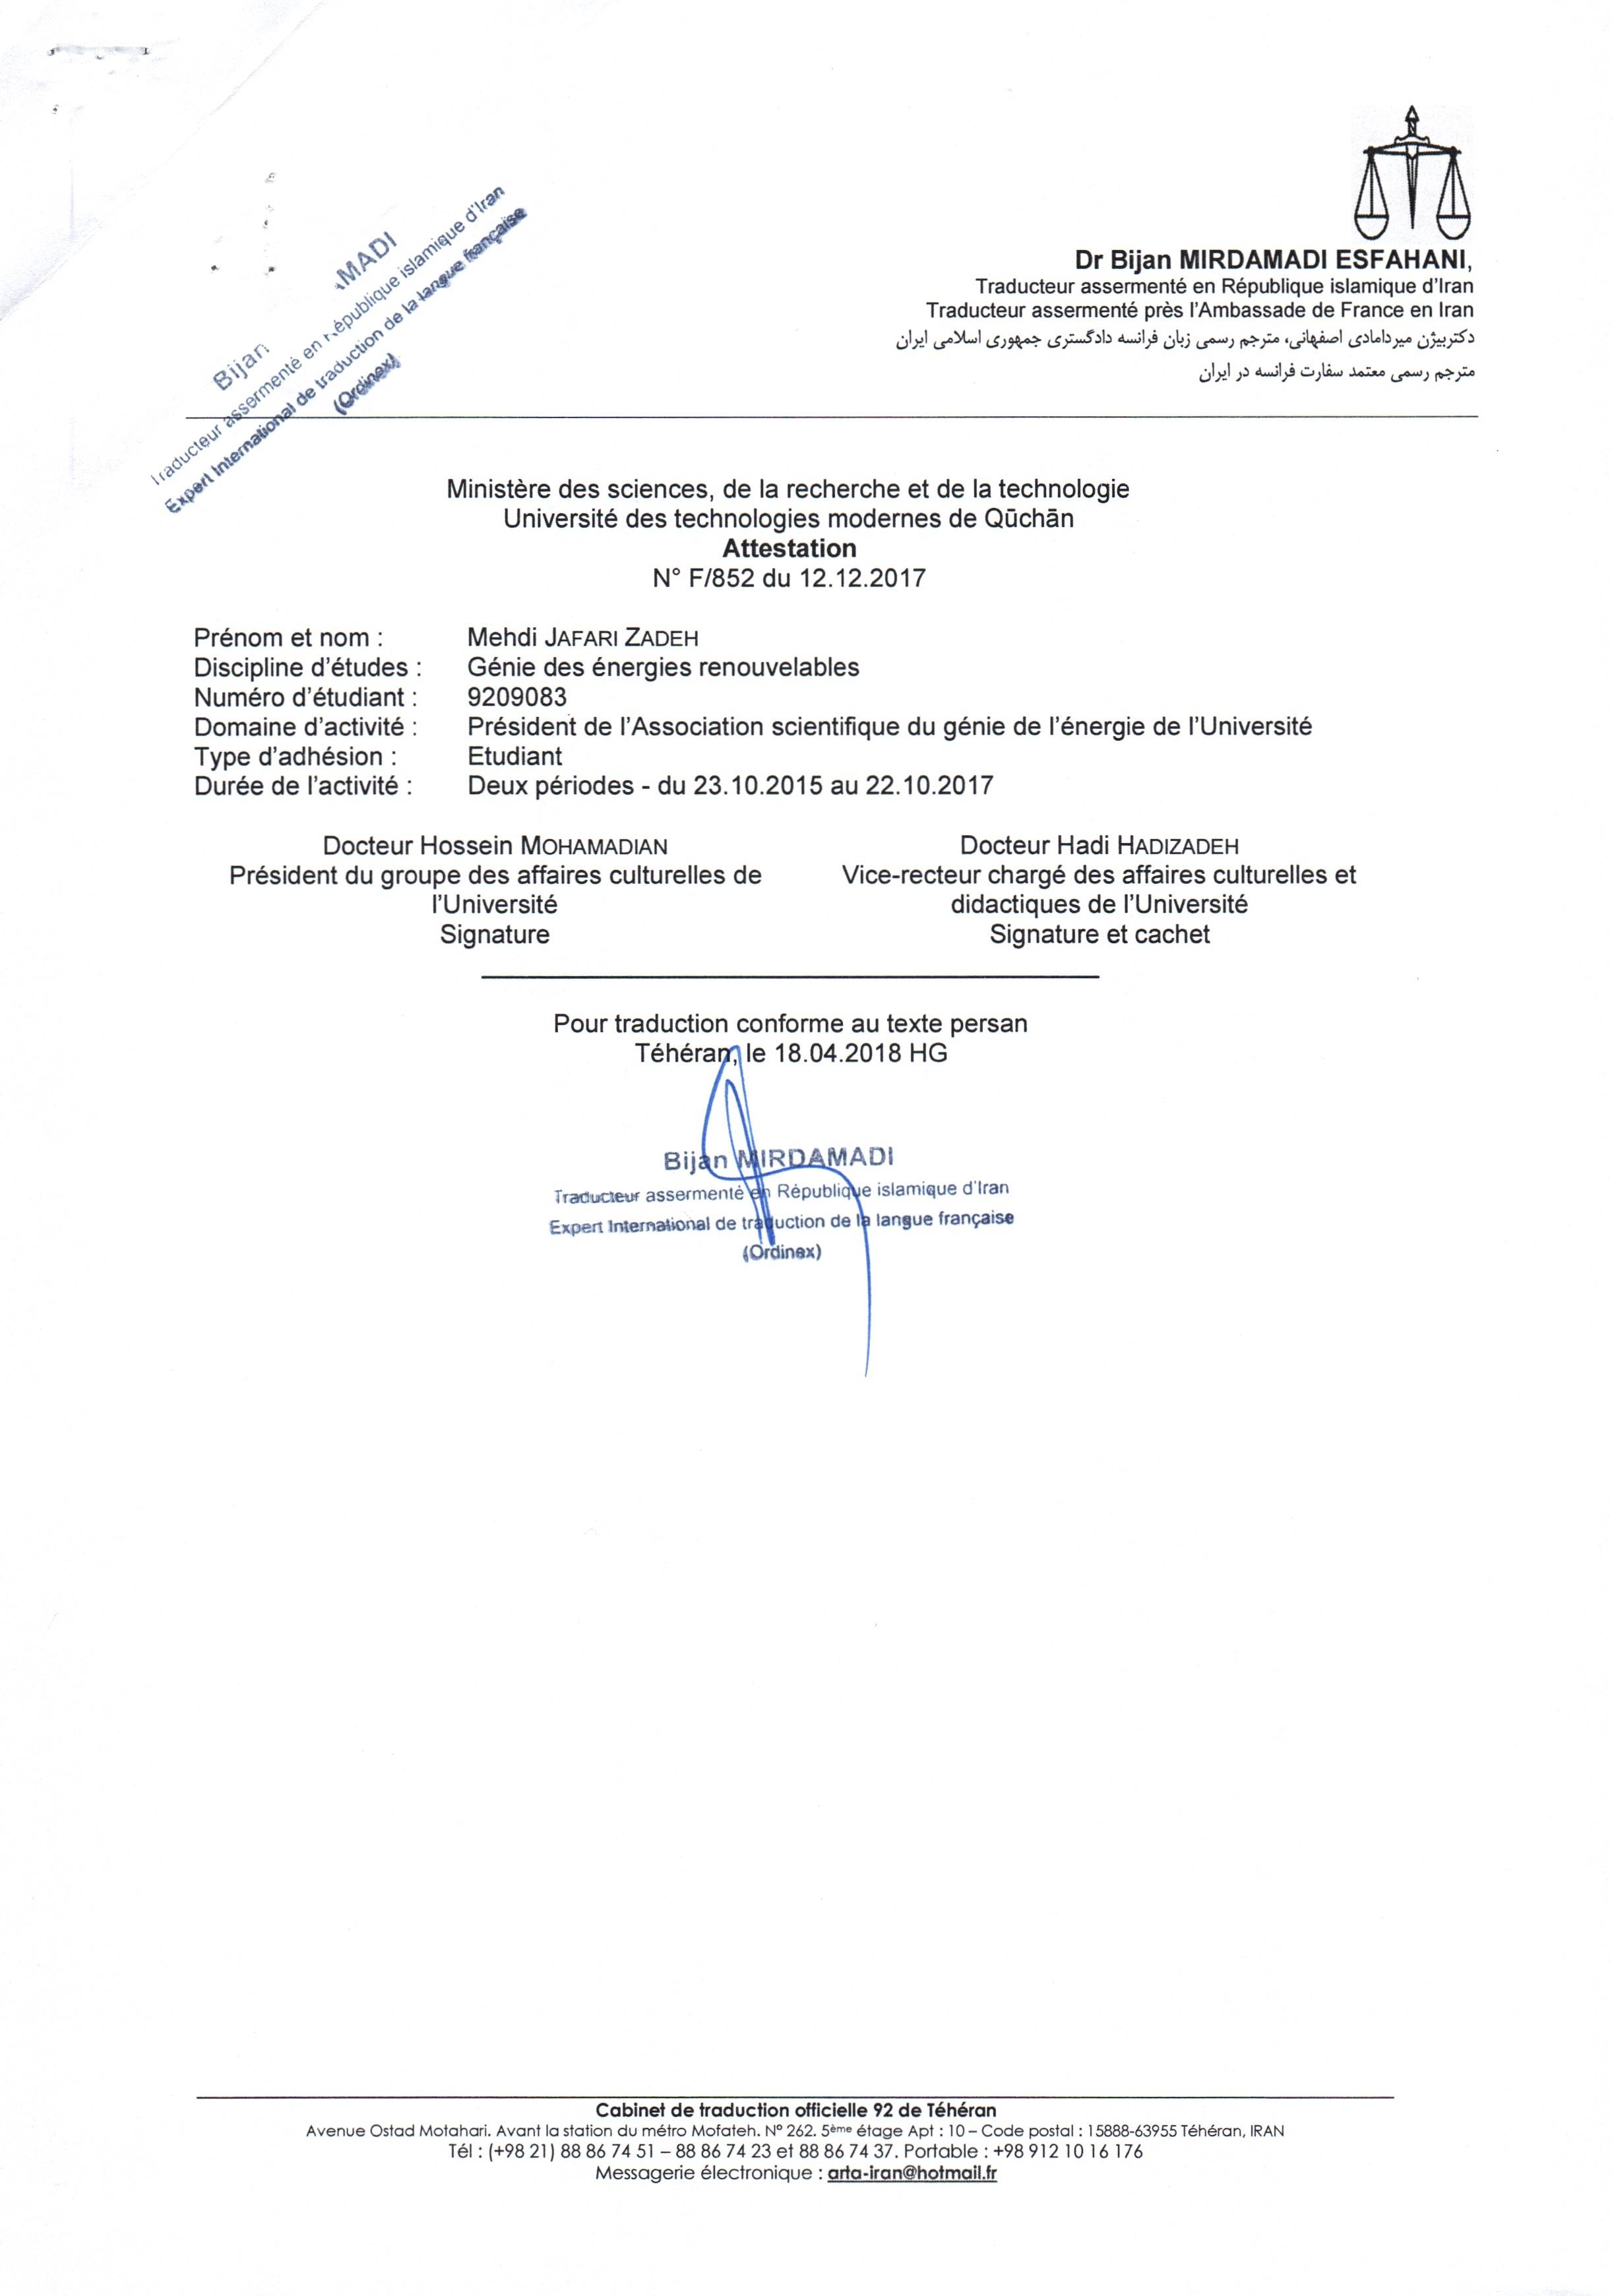
\includegraphics[width=\textwidth,height=\textheight,keepaspectratio]{../Document/Work Experience/Director of the Energy Engineering Association/12-12-2017 attestation 02.jpg}
            \footnotesize
             \href{https://github.com/jafarizadeh/CV---lettre/tree/079f60796b41475881d7ba4a70abc3254d3dd466/Document/Work%20Experience/Director%20of%20the%20Energy%20Engineering%20Association}{Veuillez cliquer ici pour accéder au document sur GitHub}.
        \end{center}


% =========================================================
% =============== Projets ===============
% =========================================================

    \section{Projets}
    % 4.1 Co-auteur
    \subsection{Co-auteur}

    Pendant mes études à l'université, j'ai coécrit un guide complet sur l'audit énergétique pour les étudiants en ingénierie de l'énergie, sous la direction du Dr Majid Mahdavian. Ce projet consistait à collecter et analyser des données statistiques étendues ainsi que des articles académiques liés aux audits énergétiques. Mes responsabilités incluaient la synthèse de ces informations dans un format clair et accessible qui servirait de ressource précieuse pour les étudiants. Le livre, publié en 2019, a été reconnu pour son approche rigoureuse et son utilité pratique dans le cours d'audit énergétique à l'Université de Quchan.

    Collaborer avec le Dr Mahdavian a été une expérience enrichissante qui a considérablement amélioré mes compétences en recherche et en analyse. Sa confiance en mes capacités m'a permis de jouer un rôle clé dans le projet, de la collecte des données à la finalisation du contenu. Cette expérience a non seulement approfondi ma compréhension des concepts d'ingénierie énergétique, mais a également affiné ma capacité à transmettre des informations techniques complexes de manière à la fois complète et adaptée aux étudiants.
    \newline
    \newline
    \textit {Note: La documentation de cette collaboration peut être trouvée dans les pages suivantes.}
    \newline
    \newline

    \newpage

        \begin{center}
            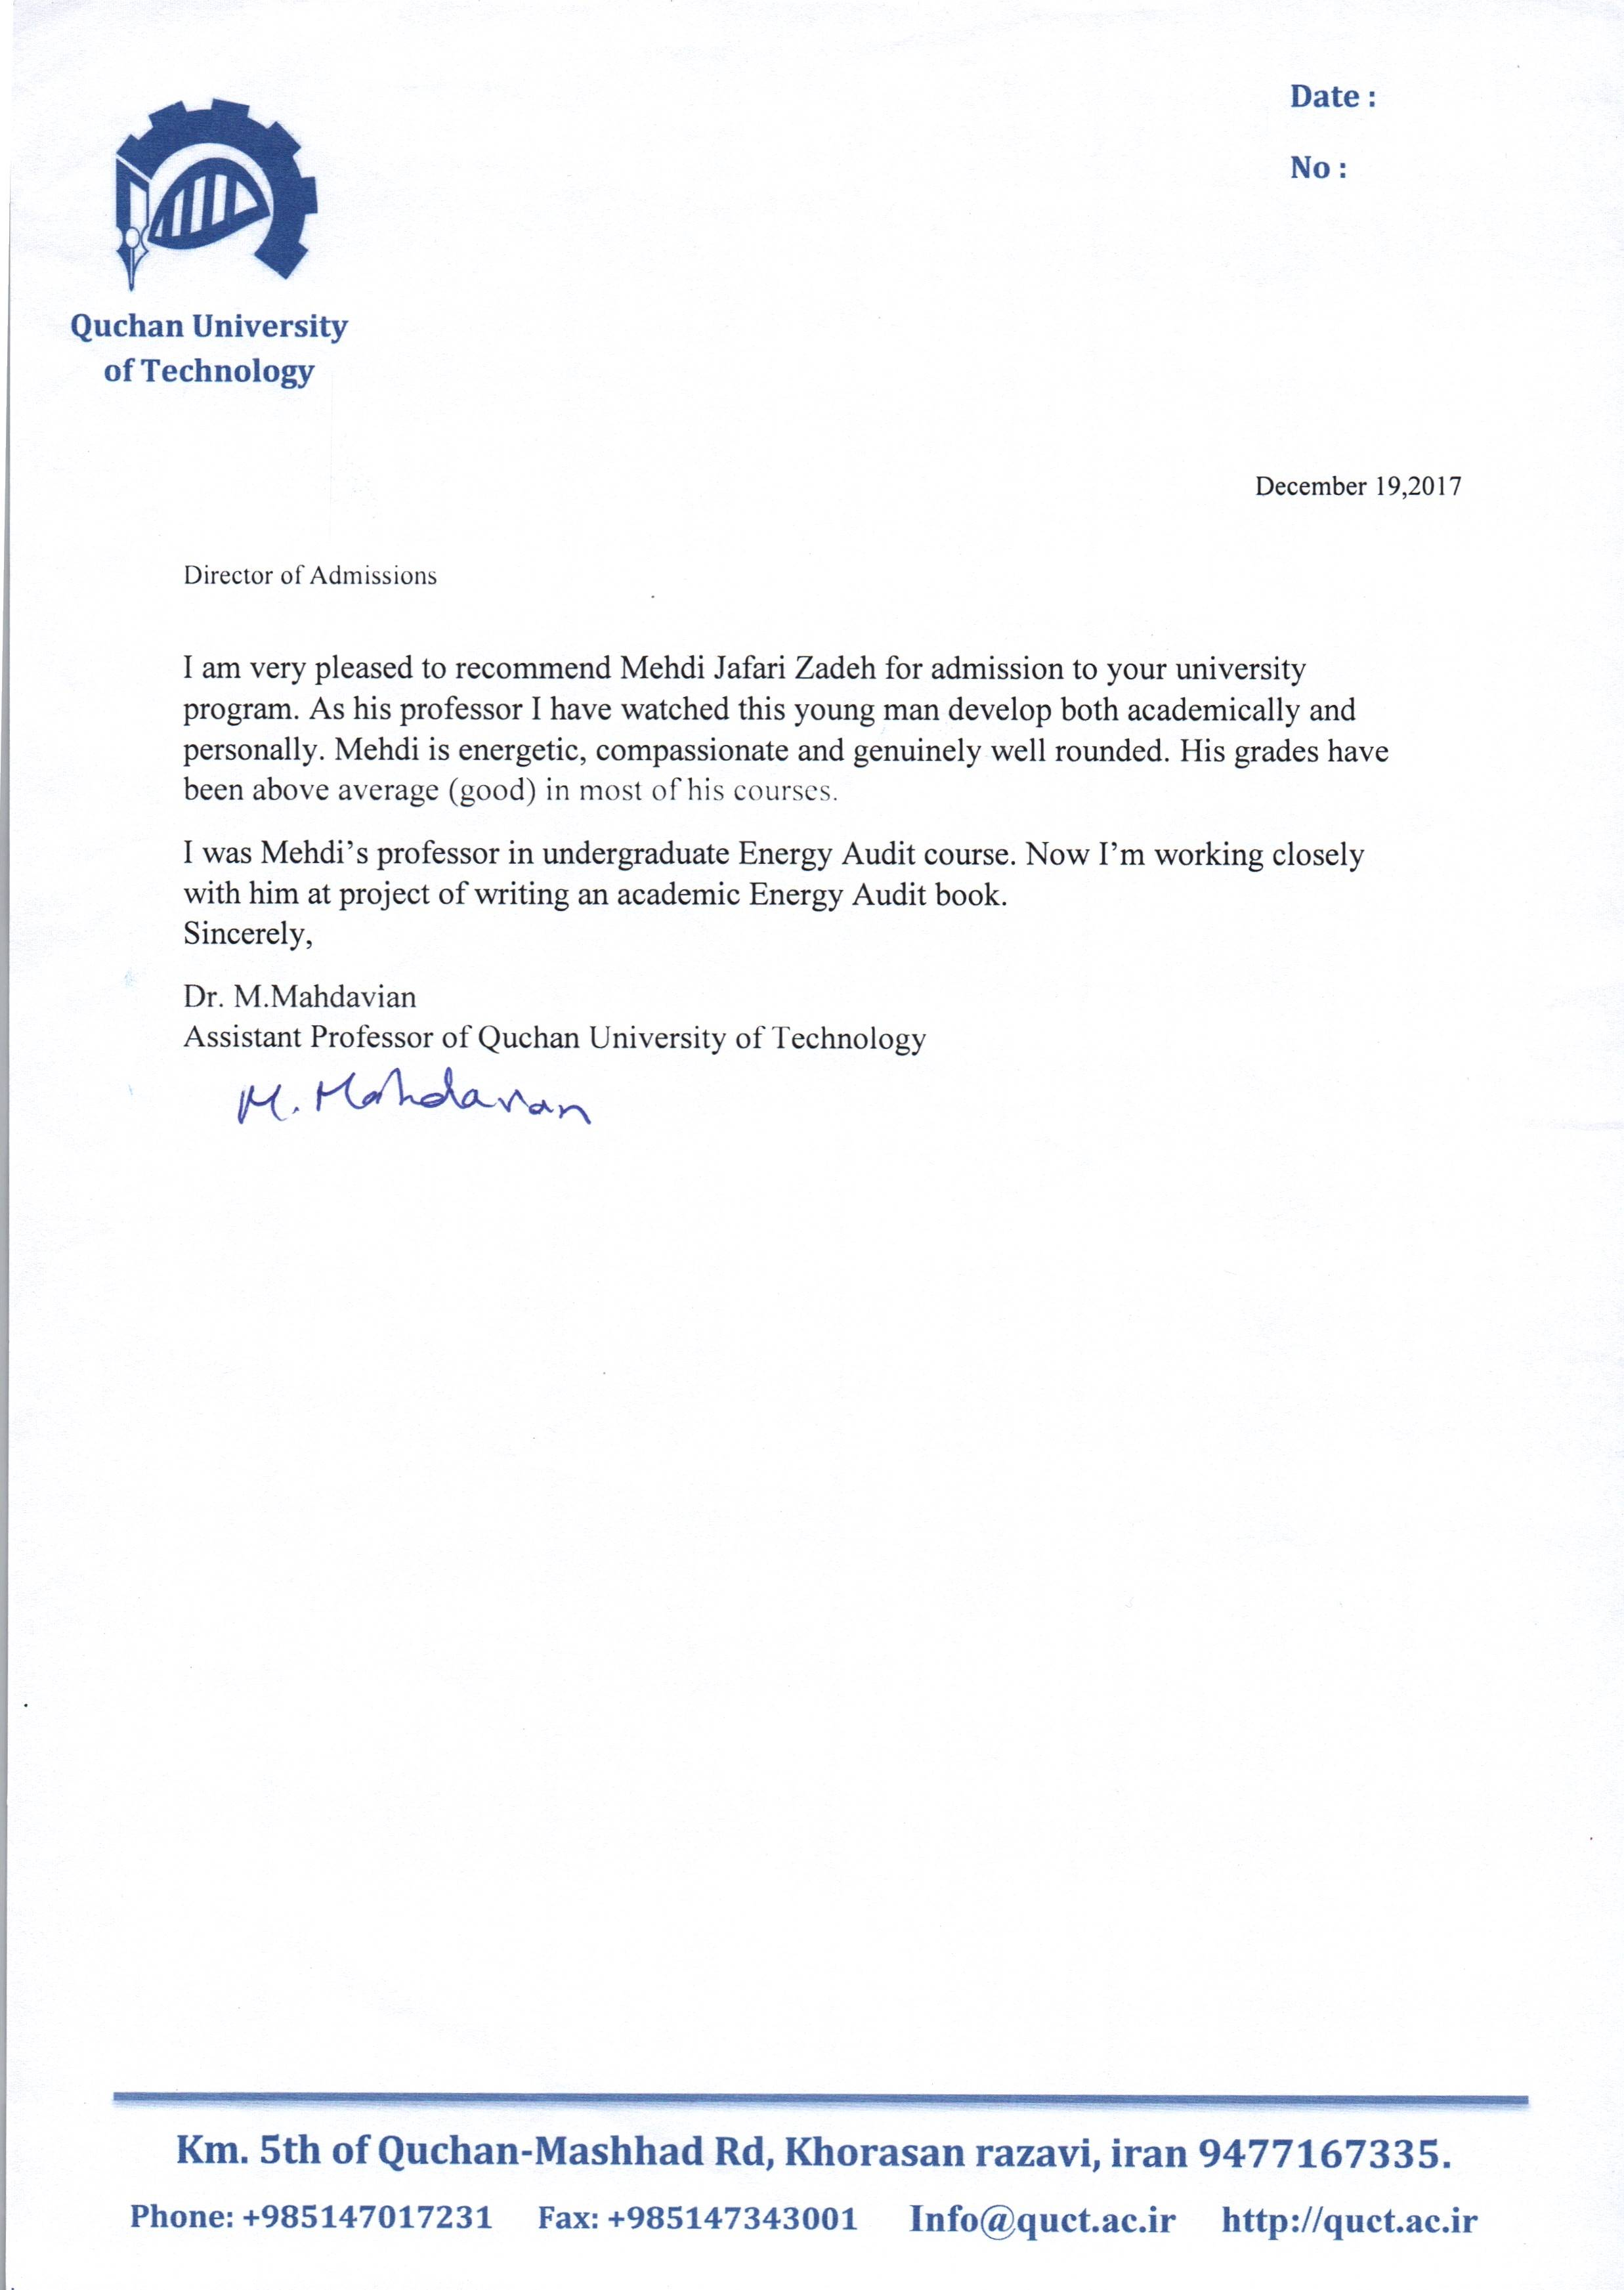
\includegraphics[width=\textwidth,height=\textheight,keepaspectratio]{../Document/Projets/Co-author/19-12-2017 lettre de recommandation - Dr. Mahdavian.jpg}
            \footnotesize
             \href{https://github.com/jafarizadeh/CV---lettre/tree/a64fa195620766a9cf39fd42a2fd963779d13f6f/Document/Projets/Co-author}{Veuillez cliquer ici pour accéder au document sur GitHub}.
        \end{center}
    


    \subsection{Développement d'un Système de Base de Données}

    \href{https://github.com/jafarizadeh/CV---lettre/tree/a64fa195620766a9cf39fd42a2fd963779d13f6f/Document/Projets/Co-author}{Veuillez cliquer ici pour accéder au document sur GitHub}.
    
    \subsection{Génération et résolution de labyrinthes}

    \href{https://github.com/jafarizadeh/CV---lettre/tree/a64fa195620766a9cf39fd42a2fd963779d13f6f/Document/Projets/Co-author}{Veuillez cliquer ici pour accéder au document sur GitHub}.
    
    \subsection{Graphe dual d’un maillage}

    \href{https://github.com/jafarizadeh/CV---lettre/tree/a64fa195620766a9cf39fd42a2fd963779d13f6f/Document/Projets/Co-author}{Veuillez cliquer ici pour accéder au document sur GitHub}.
    
    \subsection{Affichage et générateur de grille de mots croisés}

    \href{https://github.com/jafarizadeh/CV---lettre/tree/a64fa195620766a9cf39fd42a2fd963779d13f6f/Document/Projets/Co-author}{Veuillez cliquer ici pour accéder au document sur GitHub}.
    
   
    

    

    \newpage
% =========================================================
% ============ Course Completion Certificates =============
% =========================================================


\section{Certificats de Fin de Cours}

    % 5.1 CCNA 200-301
    \subsection{CCNA 200-301}

    J'ai complété un cours de formation intensif de 130 heures pour devenir Cisco Certified Network Associate (CCNA) (200-301) via Udemy, dispensé par M. Arash Deljoo. Ce programme intensif s'est déroulé sur deux mois, avec pour objectif d'équiper les participants des connaissances essentielles et des compétences pratiques en matière de fondamentaux des réseaux, d'accès réseau, de connectivité IP, de services IP, de fondamentaux de la sécurité, ainsi que d'automatisation et de programmabilité. Le cours était structuré pour fournir à la fois des cadres théoriques et une expérience pratique, en préparation à la configuration, la gestion et le dépannage réussis des réseaux Cisco.

    Sous la direction de M. Arash Deljoo, qui a démontré une expertise approfondie des principes de réseautage, la formation a mis l'accent sur des applications et des scénarios réels. Cette préparation a jeté une base solide pour la mise en œuvre et l'administration des solutions Cisco, contribuant de manière significative à mon efficacité technique et à ma préparation aux environnements réseau opérationnels.
    \newline
    \newline
    
        \begin{center}
            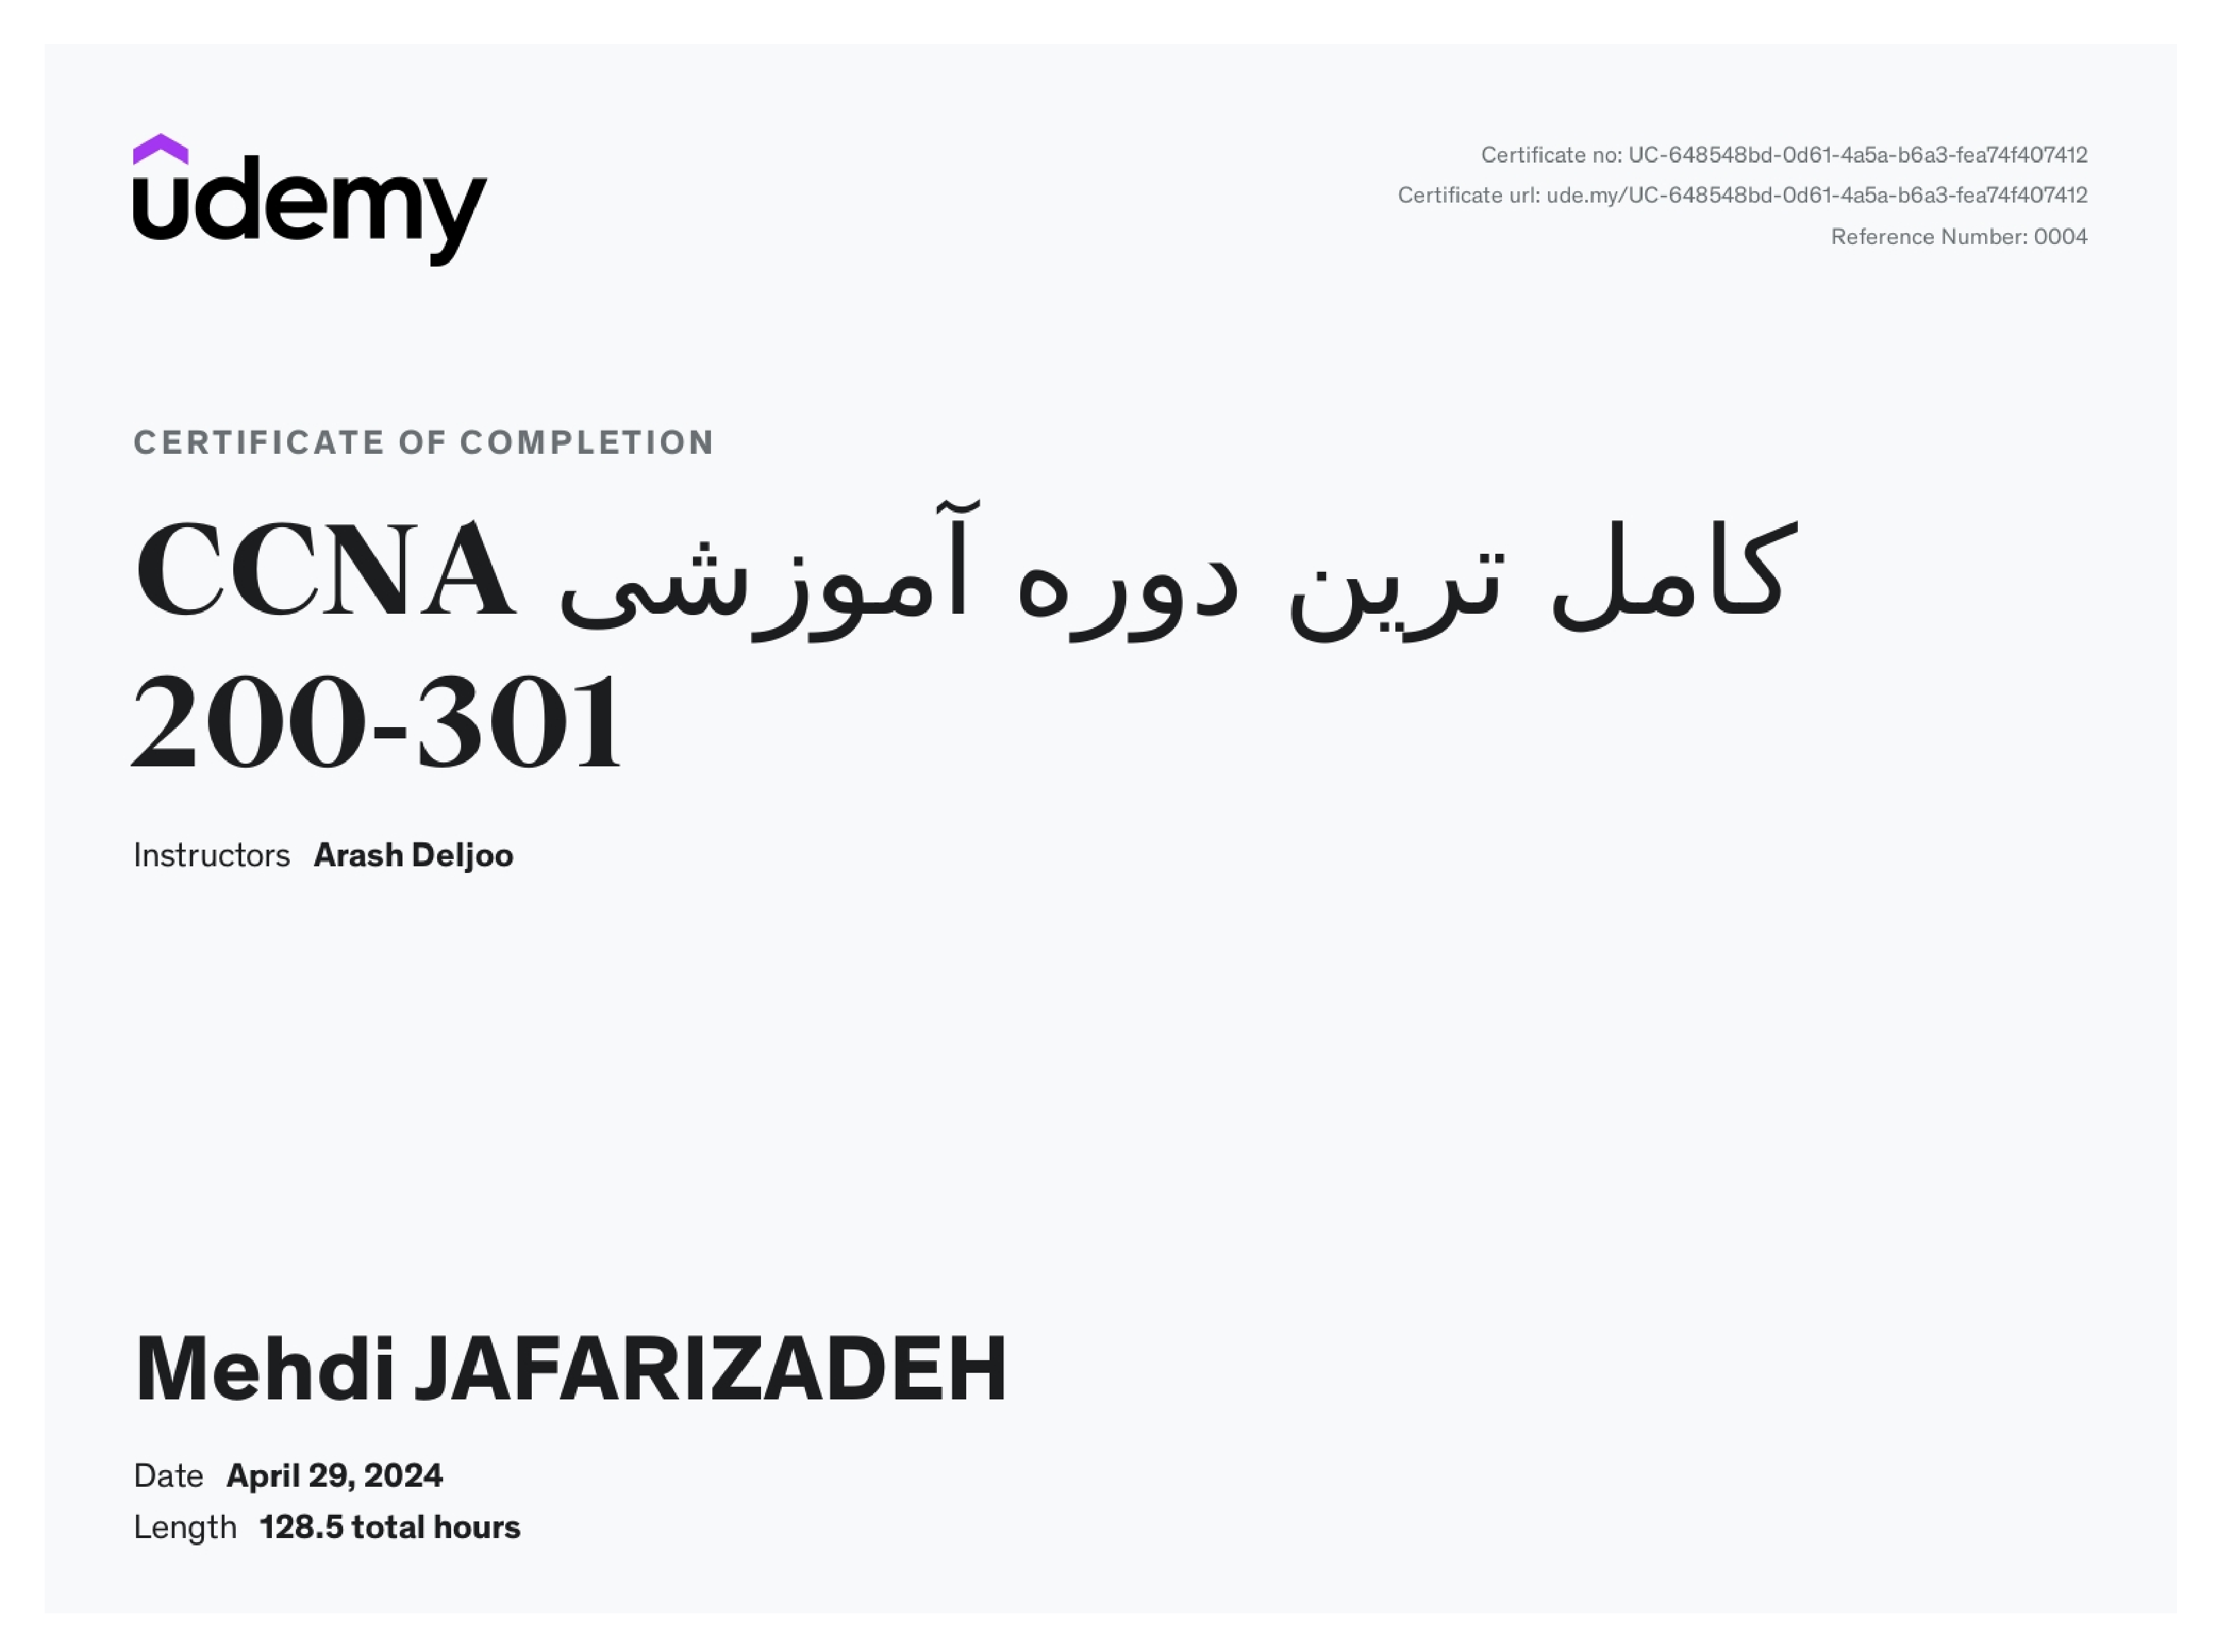
\includegraphics[width=\textwidth,height=\textheight,keepaspectratio]{../Document/Certificats de Fin de Cours/CCNA 200-301/CCNA 200-301.pdf}
            \footnotesize
             \href{https://github.com/jafarizadeh/CV---lettre/tree/a64fa195620766a9cf39fd42a2fd963779d13f6f/Document/Course%20Completion%20Certificates/CCNA%20200-301}{Veuillez cliquer ici pour accéder au document sur GitHub}.
        \end{center}

    \newpage
    
    % 5.2 CCNP ENARSI 300-410
    \subsection{CCNP ENARSI 300-410}
    \par
    Suite à ma réussite à la certification CCNA 200-301, j'ai approfondi mes compétences en réseautage en suivant le cours CCNP ENARSI (Implementing Cisco Enterprise Advanced Routing and Services) via Udemy, dispensé par M. Arash Deljo. Cette formation complète s'est déroulée sur environ 134 heures, durant lesquelles je me suis plongé dans des sujets spécialisés tels que le routage avancé, les services VPN, ainsi que la sécurité et les services d'infrastructure. Au cours de deux mois, j'ai assimilé rigoureusement le programme, ce qui m'a permis d'acquérir l'expertise nécessaire pour exceller à l'examen de certification CCNP ENARSI.
    \newline
    \newline

        \begin{center}
            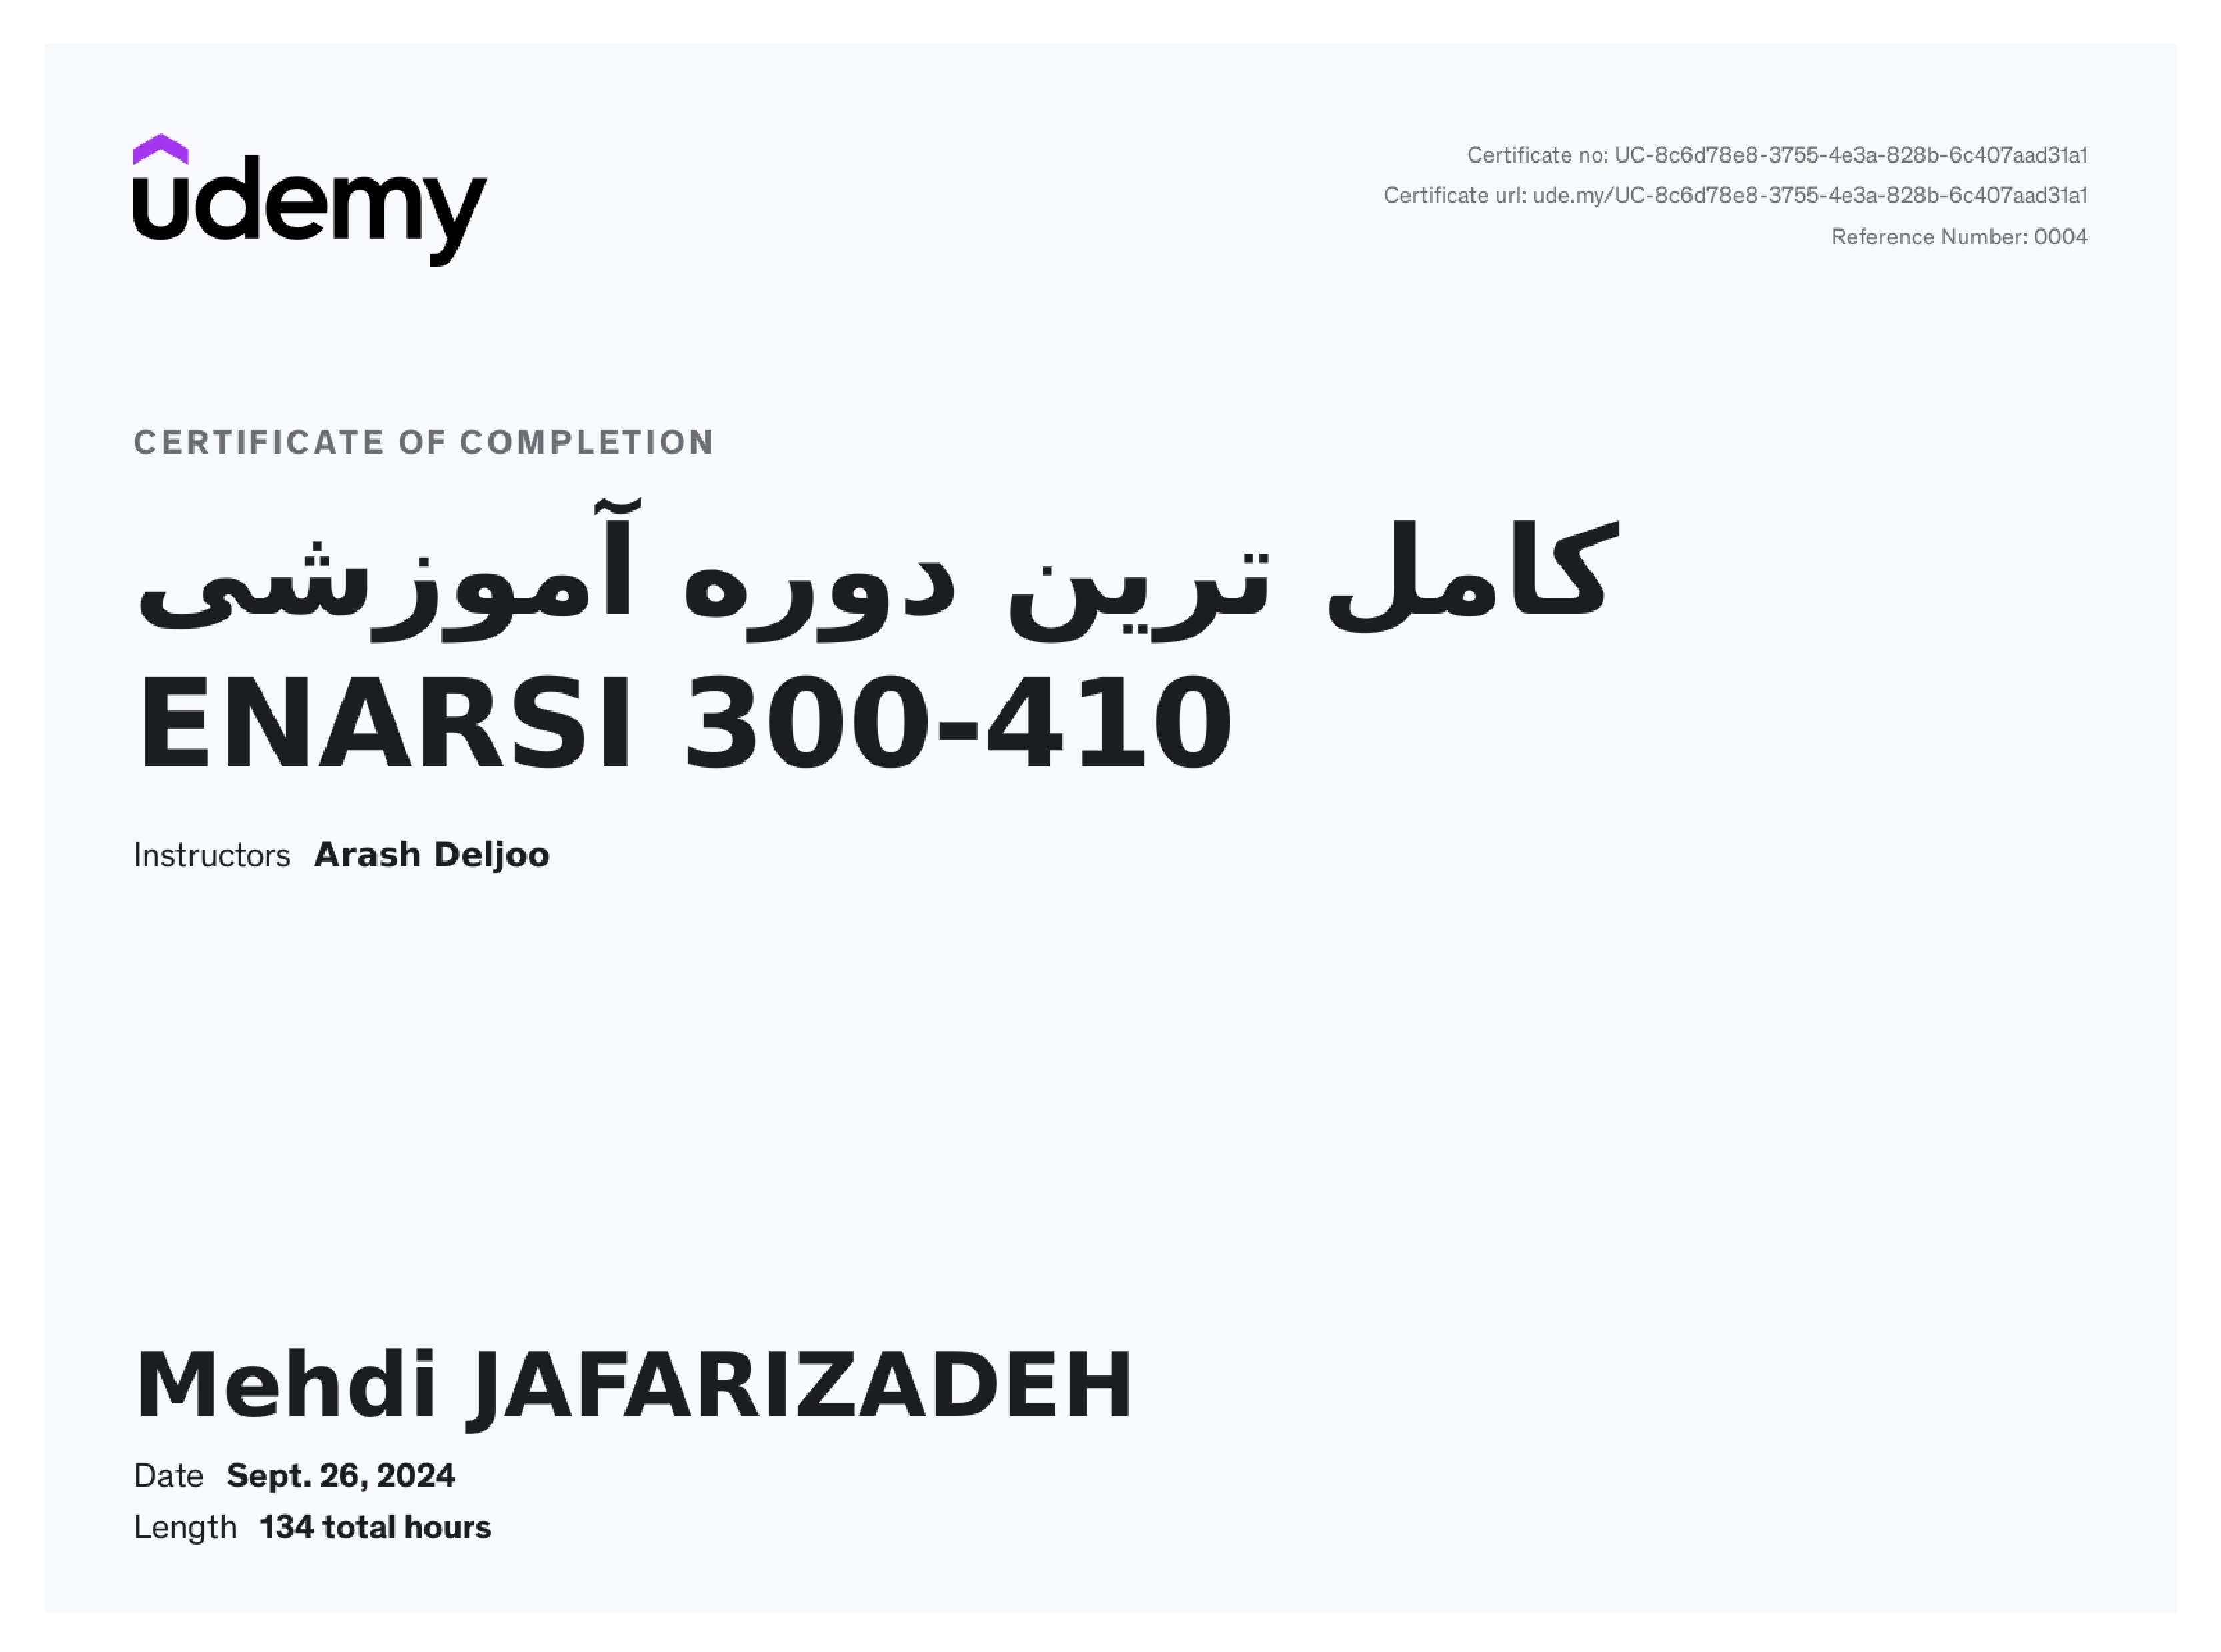
\includegraphics[width=\textwidth,height=\textheight,keepaspectratio]{../Document/Certificats de Fin de Cours/CCNP ENARSI 300-410/CCNP ENARSI 300-410.pdf}
            \footnotesize
             \href{https://github.com/jafarizadeh/CV---lettre/tree/00df58c41988ba7488536512caee235bdb5d570d/Document/Certificats%20de%20Fin%20de%20Cours/CCNP%20ENARSI%20300-410}{Veuillez cliquer ici pour accéder au document sur GitHub}.
        \end{center}

    \newpage

    % 5.3 IT network cabling: The complete fiber optics
    \subsection{IT network cabling: The complete fiber optics}
    \par
    Certifié en 'IT Network Cabling: The Complete Fiber Optics' par Udemy, ce cours intensif m'a équipé avec une compréhension approfondie des infrastructures de câblage réseau, en mettant un accent particulier sur la fibre optique. À travers des modules détaillés, j'ai appris les principes fondamentaux de la conception, de l'installation et de la maintenance des systèmes de câbles en fibre optique, incluant des compétences pratiques sur les techniques de raccordement, la mesure de performance et le dépannage des réseaux existants. Cette formation m'a également permis de maîtriser l'utilisation d'équipements spécialisés tels que les réflectomètres optiques dans le domaine (OTDR) et les sources lumineuses pour garantir l'intégrité et l'efficacité des réseaux de communication.
    
    En complément de la théorie, le cours a offert de nombreuses simulations et projets pratiques qui m'ont préparé à gérer efficacement et de manière autonome les installations de câblage en fibre optique dans divers environnements professionnels. Grâce à cette certification, je possède désormais les compétences techniques pour contribuer à la planification et à l'exécution de projets de câblage réseau, assurant ainsi une connectivité optimale et conforme aux standards actuels du secteur. Cette expertise est cruciale pour tout professionnel IT souhaitant se spécialiser dans les infrastructures réseau avancées et les solutions de télécommunication de nouvelle génération.
    \newline
    

        \begin{center}
            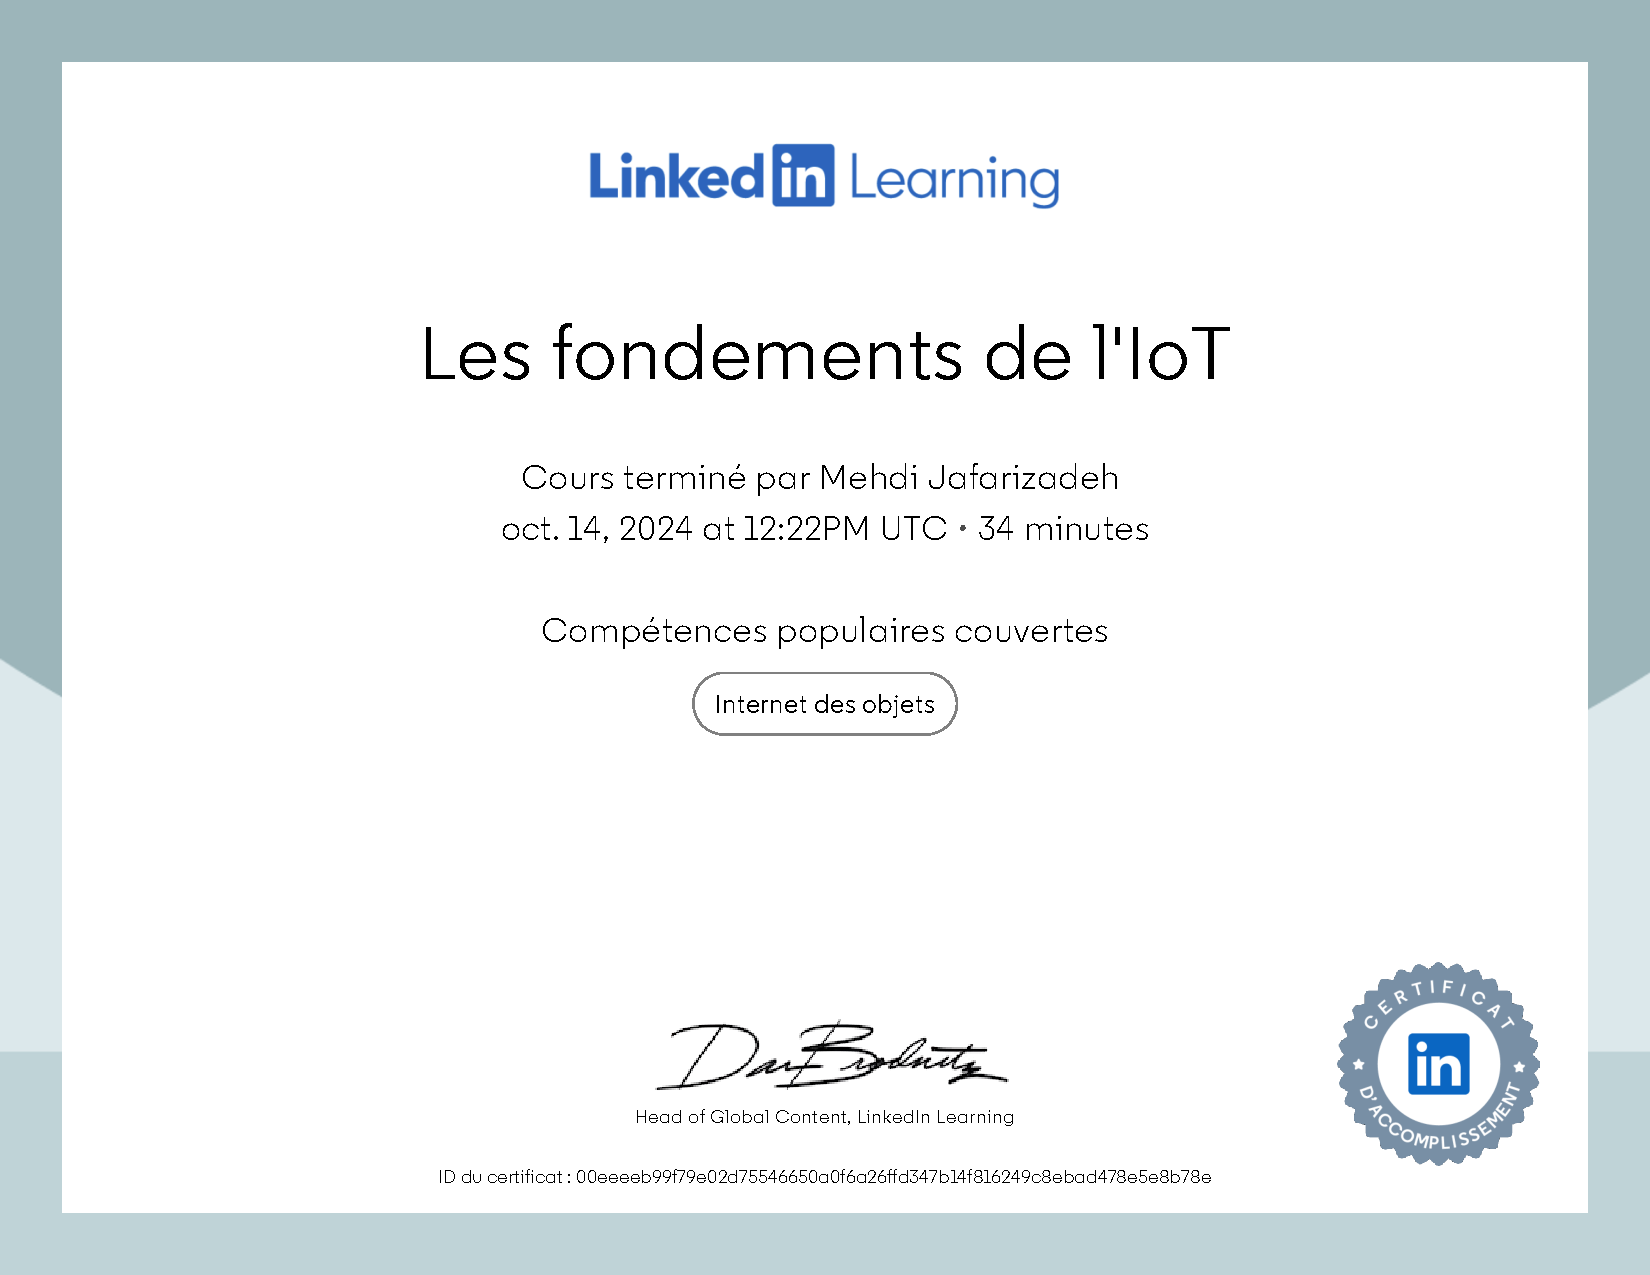
\includegraphics[width=\textwidth,height=\textheight,keepaspectratio]{../Document/Certificats de Fin de Cours/Les fondements de lIoT/Les fondements de lIoT.pdf}
            \footnotesize
             \href{https://github.com/jafarizadeh/CV---lettre/tree/00df58c41988ba7488536512caee235bdb5d570d/Document/Certificats%20de%20Fin%20de%20Cours/Les%20fondements%20de%20lIoT}{Veuillez cliquer ici pour accéder au document sur GitHub}.
        \end{center}

    \newpage
    \subsection{Devenir administrateur  administratrice reseau}

    Formation approfondie en Administration Système et Réseau, avec une expertise développée dans les infrastructures TCP/IP. Maîtrise des fondamentaux des réseaux incluant le routage, le monitoring et le contrôle d'accès dynamique. Compétences avancées en sécurité réseau, notamment dans la protection des applications et des protocoles. Acquisition d'une expertise pratique dans l'analyse de trafic avec Wireshark et la résolution des problèmes réseau.

    Spécialisation en administration Linux couvrant l'ensemble des compétences système essentielles. Maîtrise des commandes terminal, de la gestion des services système et de l'architecture Linux. Expertise développée dans la gestion du stockage, la configuration réseau sous Linux et l'implémentation des mesures de sécurité système. Cette formation complète m'a permis d'acquérir une vision globale et pratique de l'infrastructure IT moderne, associant les compétences réseau et système nécessaires à une gestion efficace des environnements professionnels.
    \newline
    
    
    \begin{center}
        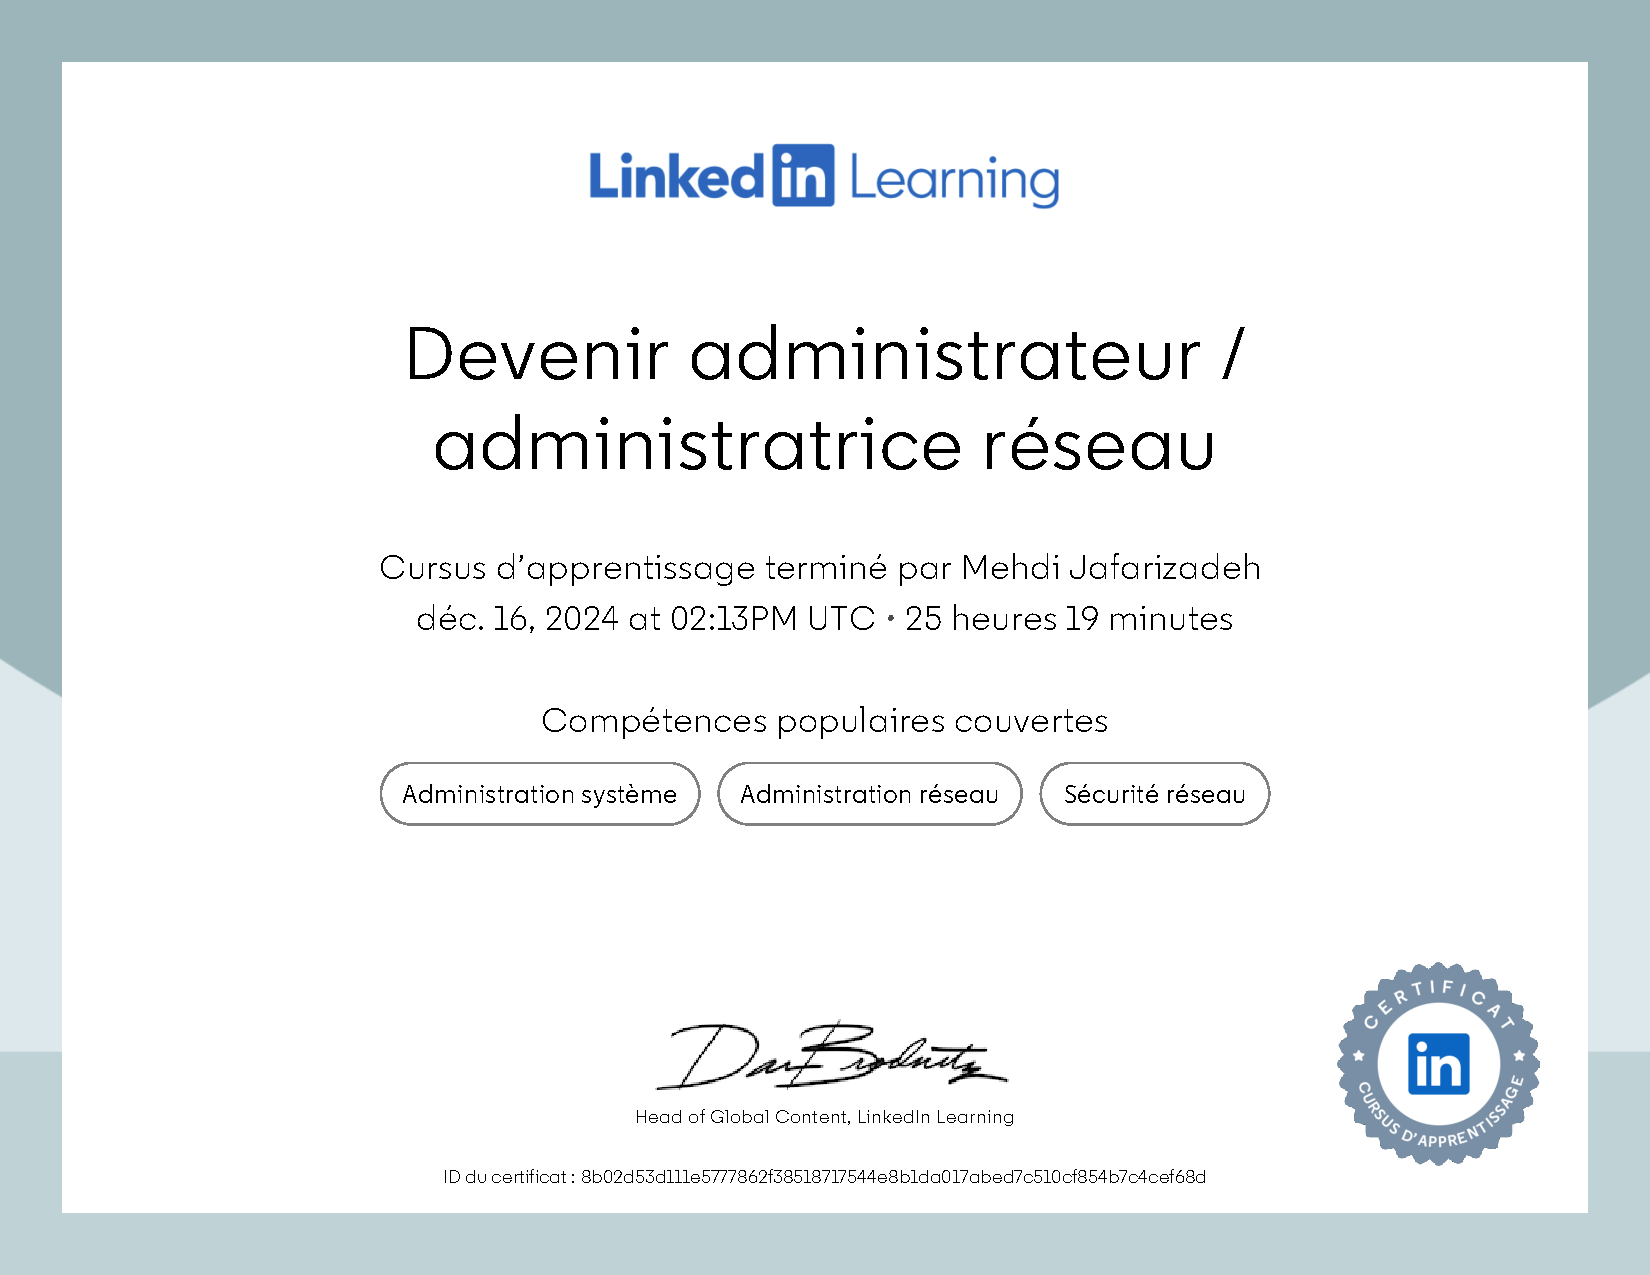
\includegraphics[width=\textwidth,height=\textheight,keepaspectratio]{../Document/Certificats de Fin de Cours/Devenir administrateur administratrice reseau/Devenir administrateur administratrice reseau.pdf}
        \footnotesize
         \href{https://github.com/jafarizadeh/CV---lettre/tree/00df58c41988ba7488536512caee235bdb5d570d/Document/Certificats%20de%20Fin%20de%20Cours/Devenir%20administrateur%20%20administratrice%20reseau}{Veuillez cliquer ici pour accéder au document sur GitHub}.

         
    \end{center}

    \newpage
    \subsection{Devenir administrateur  administratrice systeme linux}
    \begin{center}
    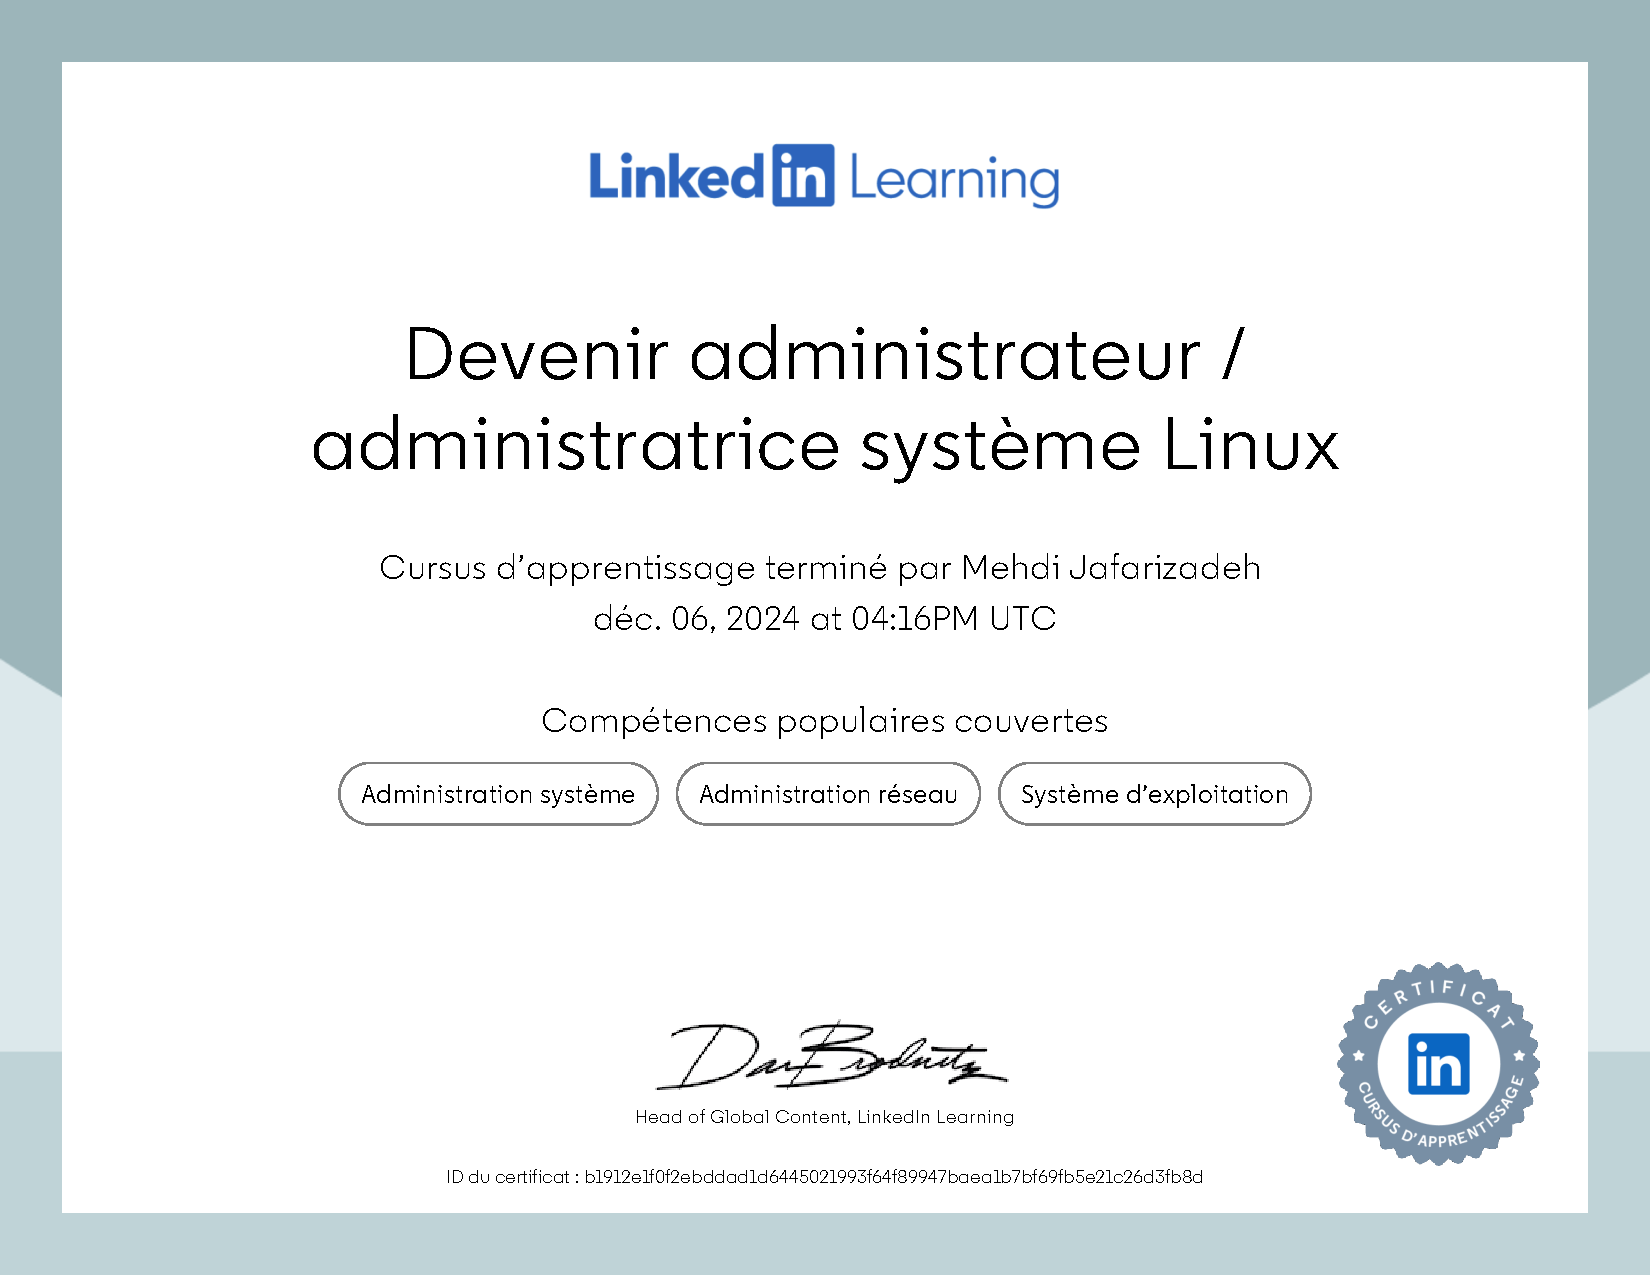
\includegraphics[width=\textwidth,height=\textheight,keepaspectratio]{../Document/Certificats de Fin de Cours/Devenir administrateur administratrice systeme Linux/Devenir administrateur administratrice systeme Linux.pdf}
         \href{https://github.com/jafarizadeh/CV---lettre/tree/00df58c41988ba7488536512caee235bdb5d570d/Document/Certificats%20de%20Fin%20de%20Cours/Devenir%20administrateur%20%20administratrice%20systeme%20Linux}{Veuillez cliquer ici pour accéder au document sur GitHub}.
    
        \end{center}
    \newpage
    % 5.3 Wireshark for Beginners Capture Packets
    \subsection{Wireshark for Beginners: Capture Packets}

    En parallèle de ma formation Cisco CCNA, j'ai suivi un cours d'introduction à Wireshark via Coursera pour améliorer ma compréhension pratique de l'analyse réseau. Ce cours, intitulé "Wireshark for Beginners: Capture Packets", a été déterminant dans le développement de mes compétences en surveillance et analyse du trafic réseau, un élément crucial pour une gestion et une sécurité efficaces du réseau. La formation a offert une expérience pratique avec Wireshark, m'apprenant à capturer, analyser et interpréter les paquets réseau, ce qui a considérablement amélioré mes capacités de dépannage.

    En m'appuyant sur cette base, j'ai approfondi mon expertise avec un autre cours spécialisé de Coursera, "Initiation à Wireshark pour l'analyse de paquets sous linux". Cette formation avancée s'est concentrée sur l'application des techniques d'analyse de paquets dans des environnements Linux, affinant davantage mes compétences analytiques et approfondissant ma compréhension de la dynamique réseau. Ces cours ont été essentiels pour compléter ma certification CCNA, me dotant d'un ensemble d'outils robustes pour évaluer et optimiser efficacement les performances du réseau.
    \newline
    \newline
    
        \begin{center}
            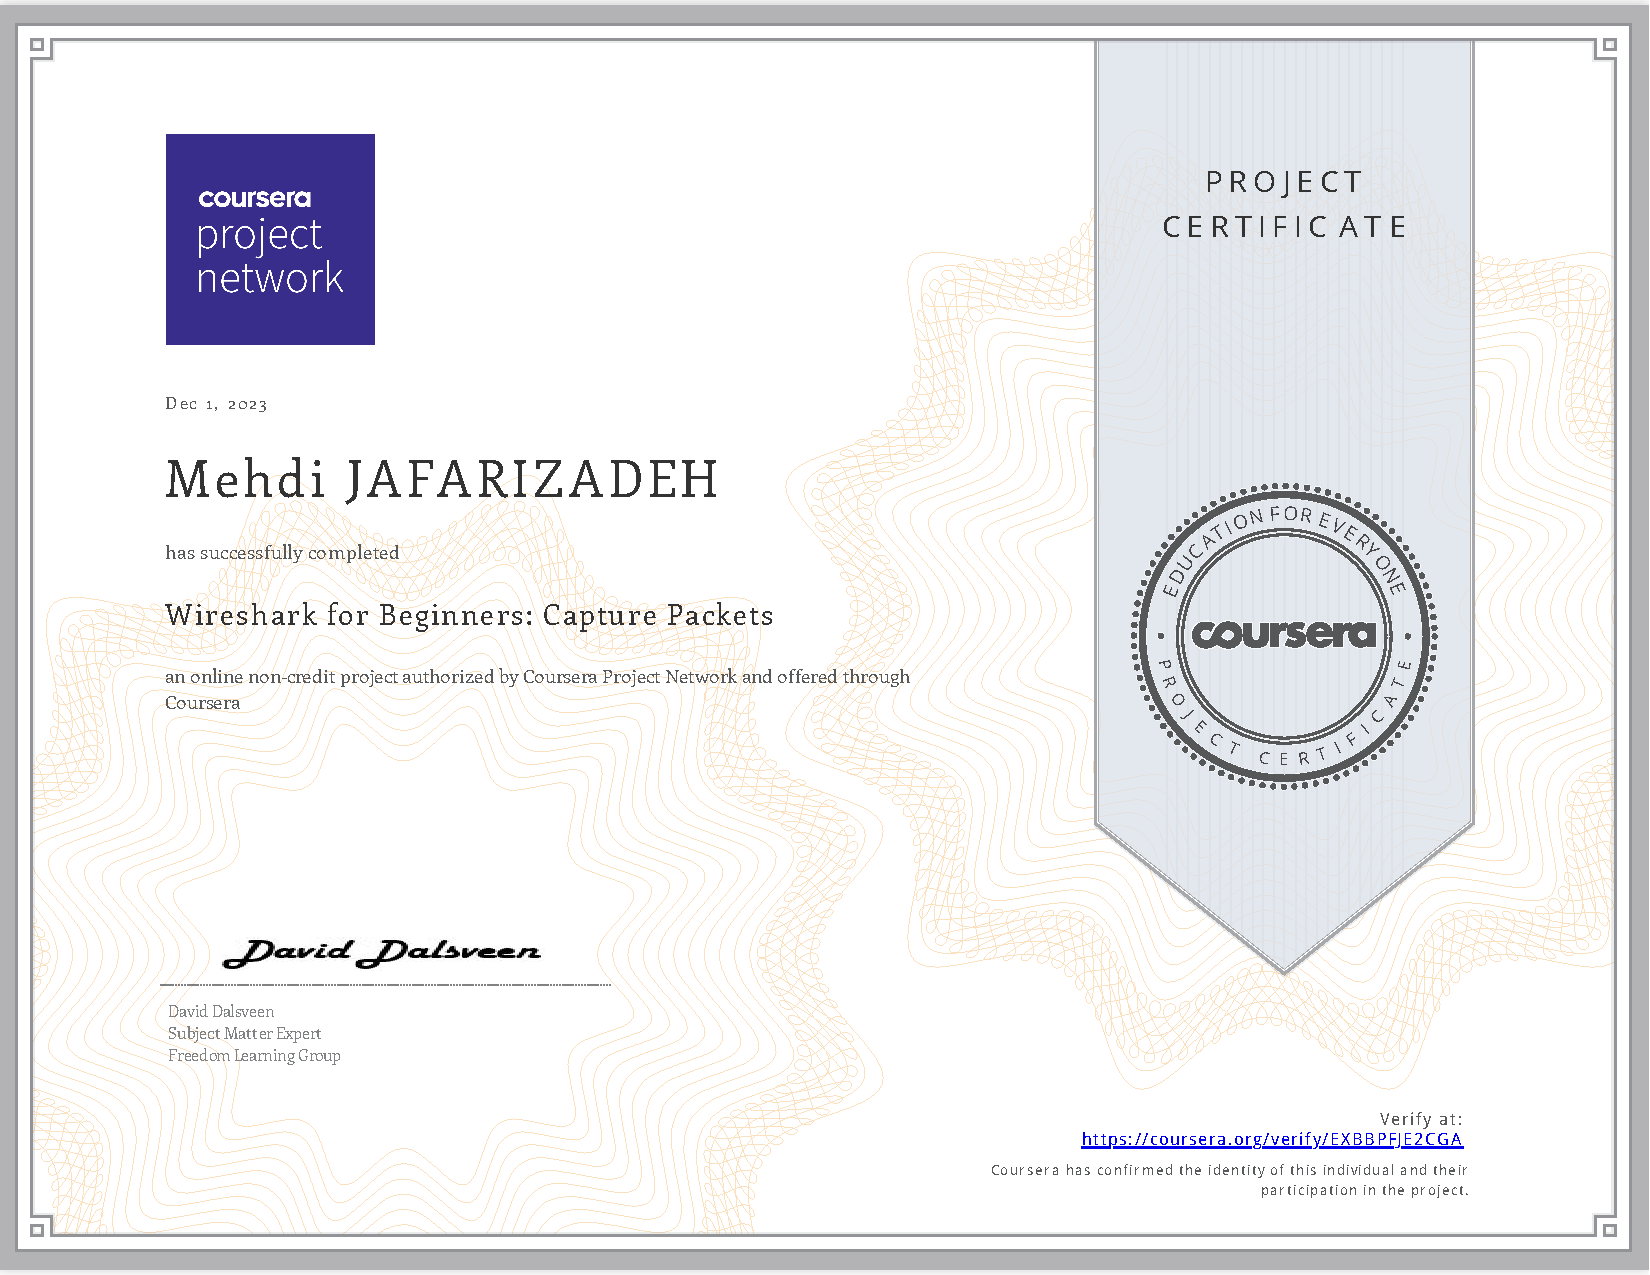
\includegraphics[width=\textwidth,height=\textheight,keepaspectratio]{../Document/Certificats de Fin de Cours/Wireshark for Beginners Capture Packets/Wireshark for Beginners Capture Packets.pdf}
            \footnotesize
             \href{https://github.com/jafarizadeh/CV---lettre/tree/00df58c41988ba7488536512caee235bdb5d570d/Document/Certificats%20de%20Fin%20de%20Cours/Wireshark%20for%20Beginners%20Capture%20Packets}{Veuillez cliquer ici pour accéder au document sur GitHub}.
        \end{center}

    \newpage
    
    % 5.4 Initiation à Wireshark pour l'analyse de paquets sous linux 
    \subsection{Initiation à Wireshark pour l'analyse de paquets sous linux}
    
        \begin{center}
            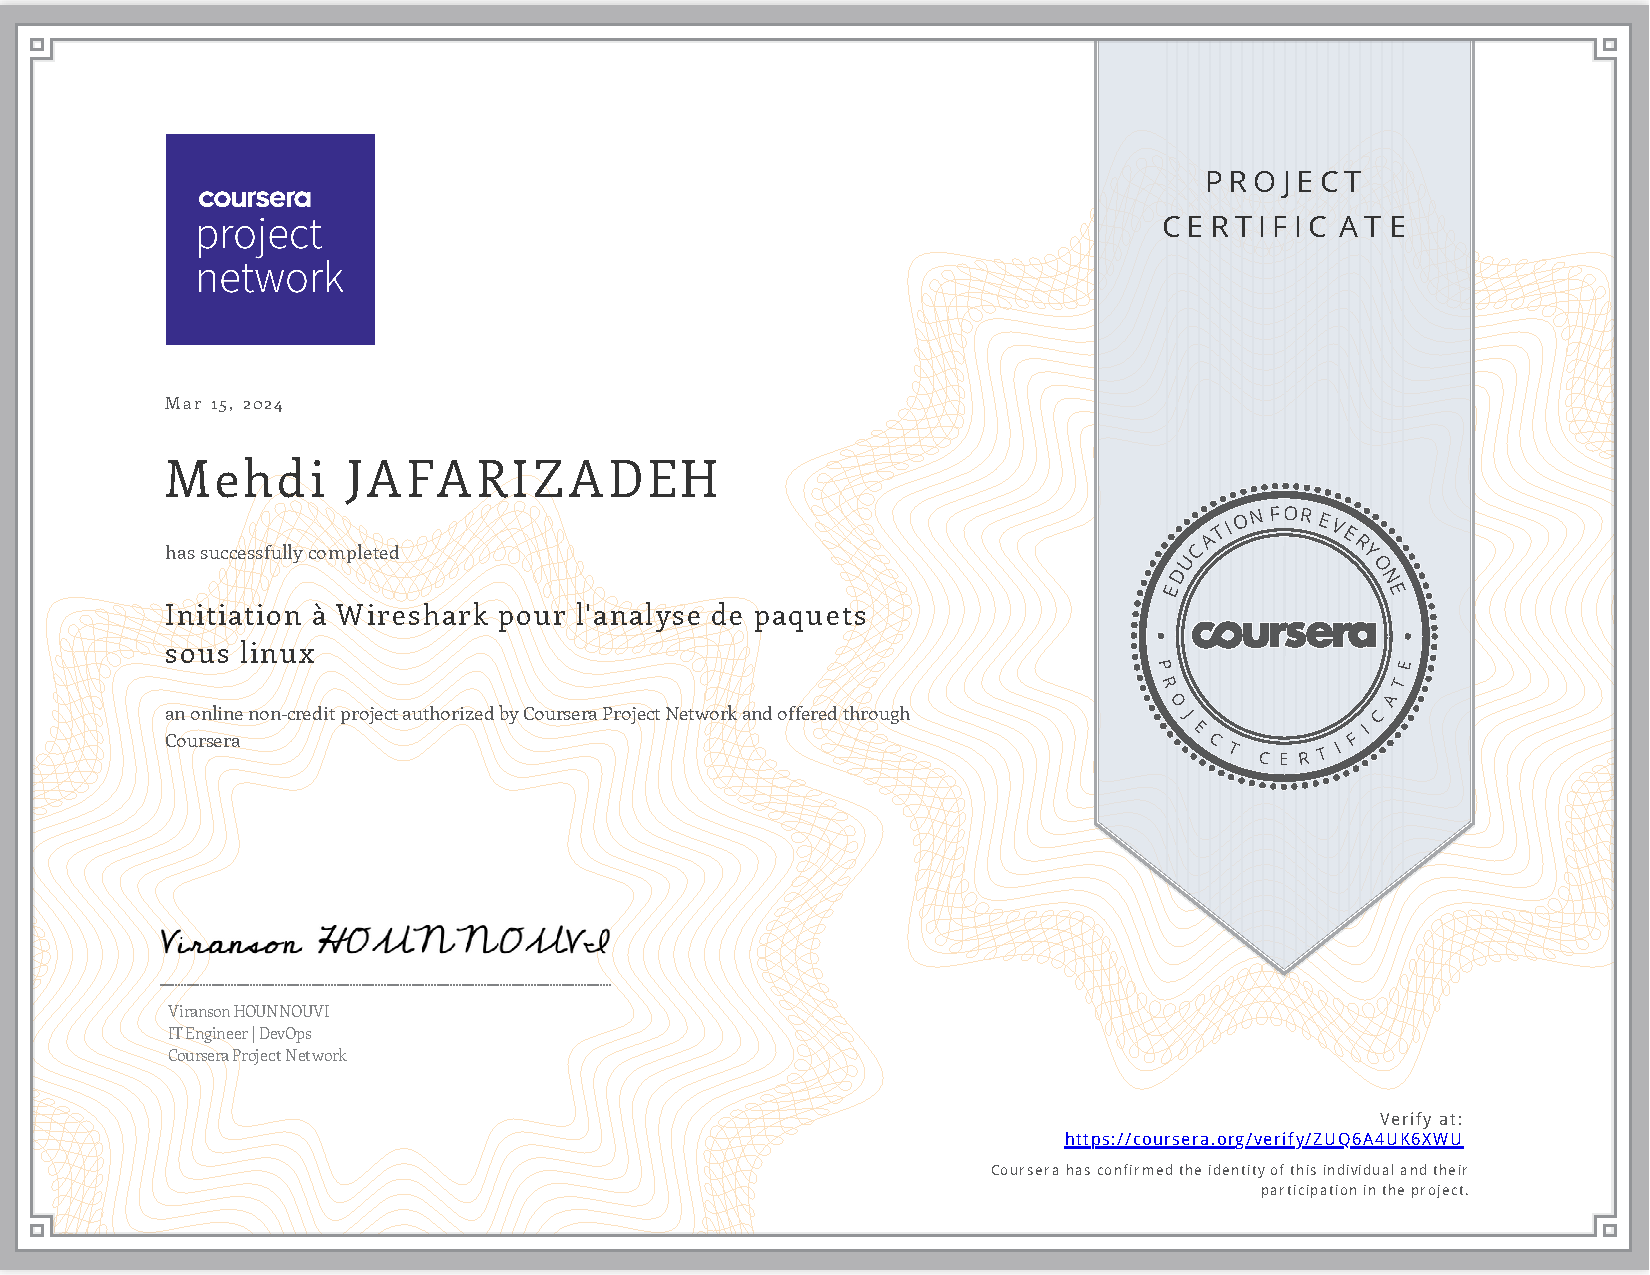
\includegraphics[width=\textwidth,height=\textheight,keepaspectratio]{../Document/Certificats de Fin de Cours/Getting Started with Wireshark for Packet Analysis on Linux/Getting Started with Wireshark for Packet Analysis on Linux.pdf}
            \footnotesize
             \href{https://github.com/jafarizadeh/CV---lettre/tree/00df58c41988ba7488536512caee235bdb5d570d/Document/Certificats%20de%20Fin%20de%20Cours/Getting%20Started%20with%20Wireshark%20for%20Packet%20Analysis%20on%20Linux}{Veuillez cliquer ici pour accéder au document sur GitHub}.
        \end{center}

    \newpage
    
 

    % 5.6 Google Cloud Fundamentals: Core Infrastructure
    \subsection{Google Cloud Fundamentals: Core Infrastructure}
    J'ai complété le cours "Google Cloud Fundamentals: Core Infrastructure" via Coursera, un programme complet de 6 heures conçu pour introduire les concepts fondamentaux et les services de Google Cloud. Ce cours couvrait des sujets critiques tels que les ressources cloud et la gestion des accès, les machines virtuelles, l'architecture réseau, les solutions de stockage cloud, les technologies de conteneurisation et le déploiement d'applications cloud. Chaque module a été élaboré pour fournir une compréhension approfondie de l'utilisation efficace des technologies Google Cloud dans des scénarios réels, améliorant ainsi ma capacité à concevoir, implémenter et gérer des solutions d'infrastructure cloud.

    La formation m'a doté de connaissances pratiques sur l'optimisation des ressources cloud et le déploiement d'applications, des compétences cruciales pour naviguer et exploiter efficacement la plateforme Google Cloud. Cette expertise est essentielle dans le cadre de mon développement technique continu et pour répondre aux besoins en infrastructure des environnements numériques modernes.
    \newline
    \newline
    \begin{center}
            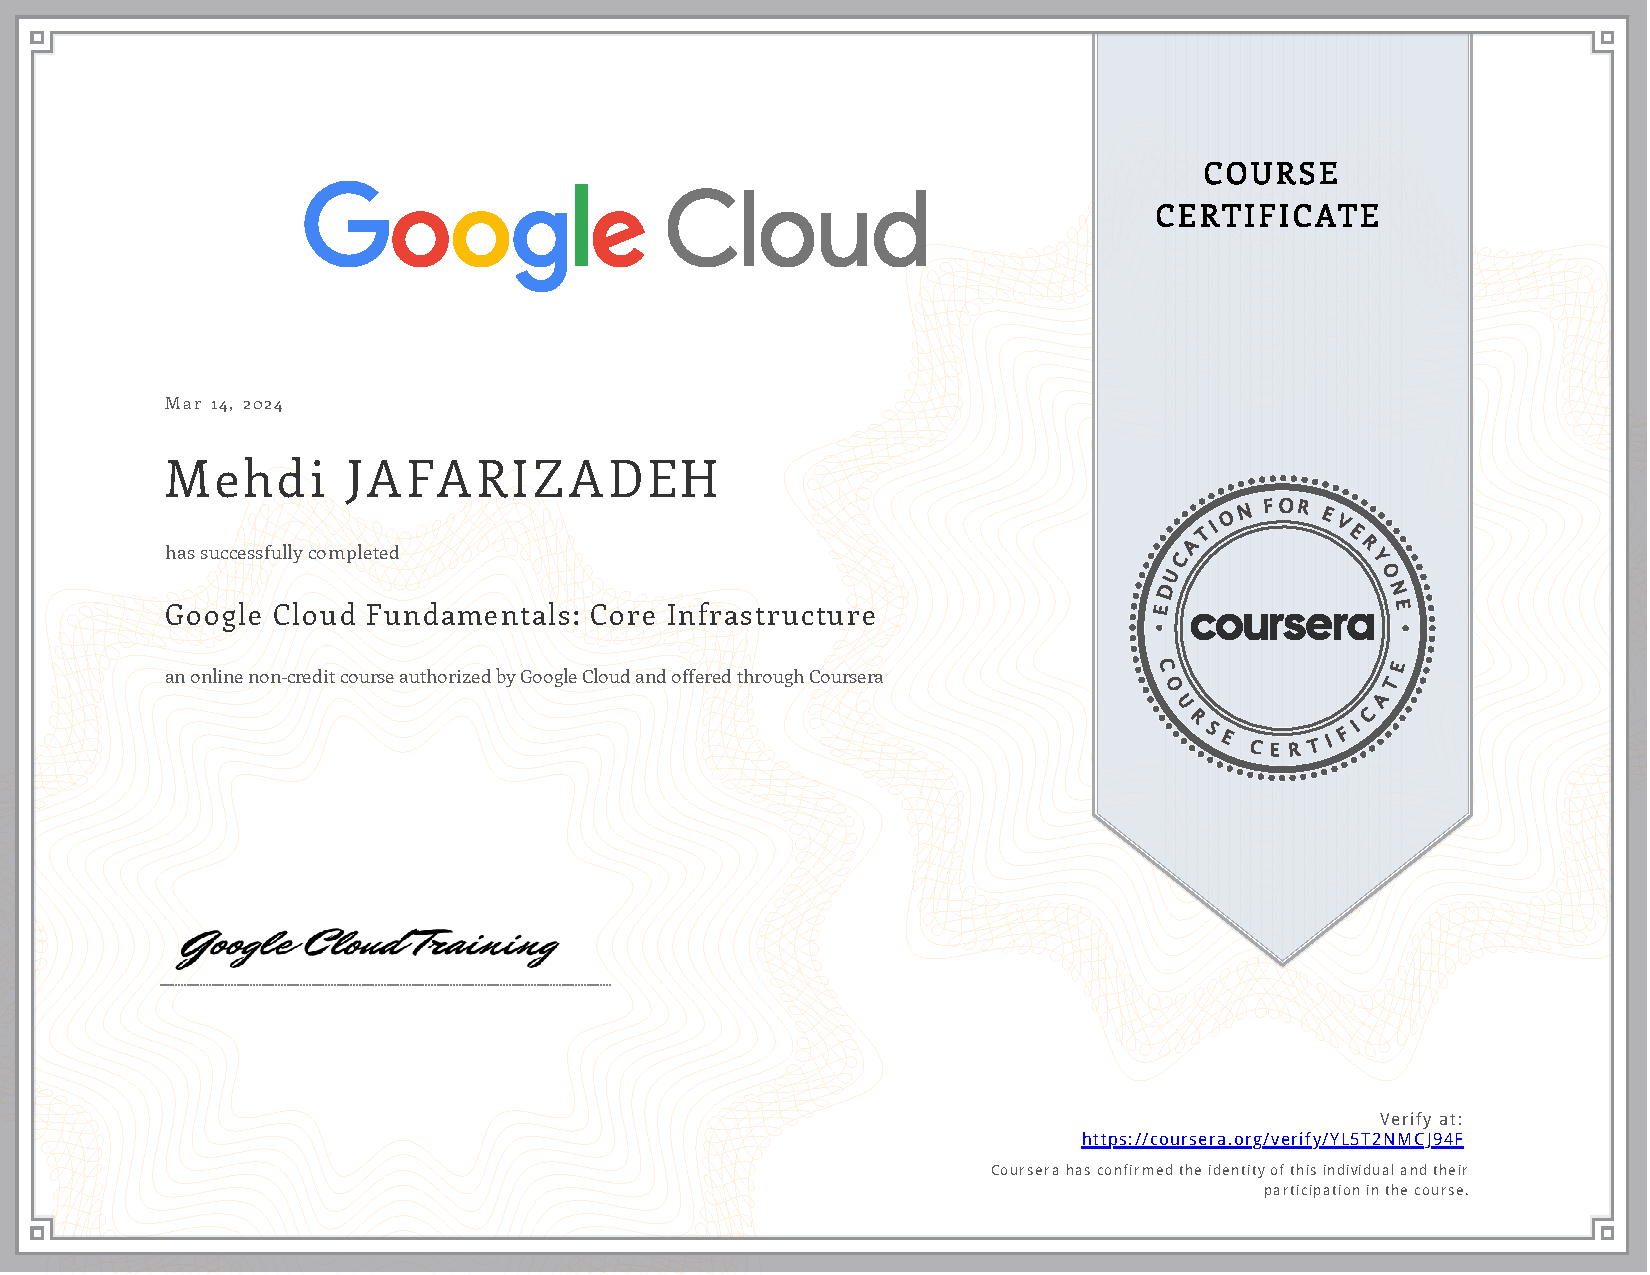
\includegraphics[width=\textwidth,height=\textheight,keepaspectratio]{../Document/Certificats de Fin de Cours/Google Cloud Fundamentals Core Infrastructure/Google Cloud Fundamentals Core Infrastructure.pdf}
            \footnotesize
             \href{https://github.com/jafarizadeh/CV---lettre/tree/00df58c41988ba7488536512caee235bdb5d570d/Document/Certificats%20de%20Fin%20de%20Cours/Google%20Cloud%20Fundamentals%20Core%20Infrastructure}{Veuillez cliquer ici pour accéder au document sur GitHub}.
        \end{center}

    \newpage

% =========================================================
% ============= Certificats d'Accomplissement =============
% =========================================================


\section{Certificats d'Accomplissement}

    % 6.1 MATLAB
    \subsection{MATLAB}
    J'ai complété avec succès un cours de formation de 30 heures en MATLAB, certifié par l'Institut Isiran, avec un score de 85 sur 100. Ce cours, achevé en octobre 2017, était axé sur le développement de compétences en MATLAB pour des applications en informatique et en ingénierie. Le programme rigoureux mettait l'accent sur les compétences pratiques en programmation, l'analyse de données et le développement d'algorithmes, me dotant des outils nécessaires pour résoudre efficacement des problèmes techniques complexes en utilisant le logiciel MATLAB.

    Cette certification souligne ma capacité à utiliser des logiciels mathématiques avancés pour améliorer la productivité et résoudre des défis pertinents pour l'industrie, reflétant une base solide tant en programmation qu'en compétences analytiques.
    \newline
    \newline
        \begin{center}
            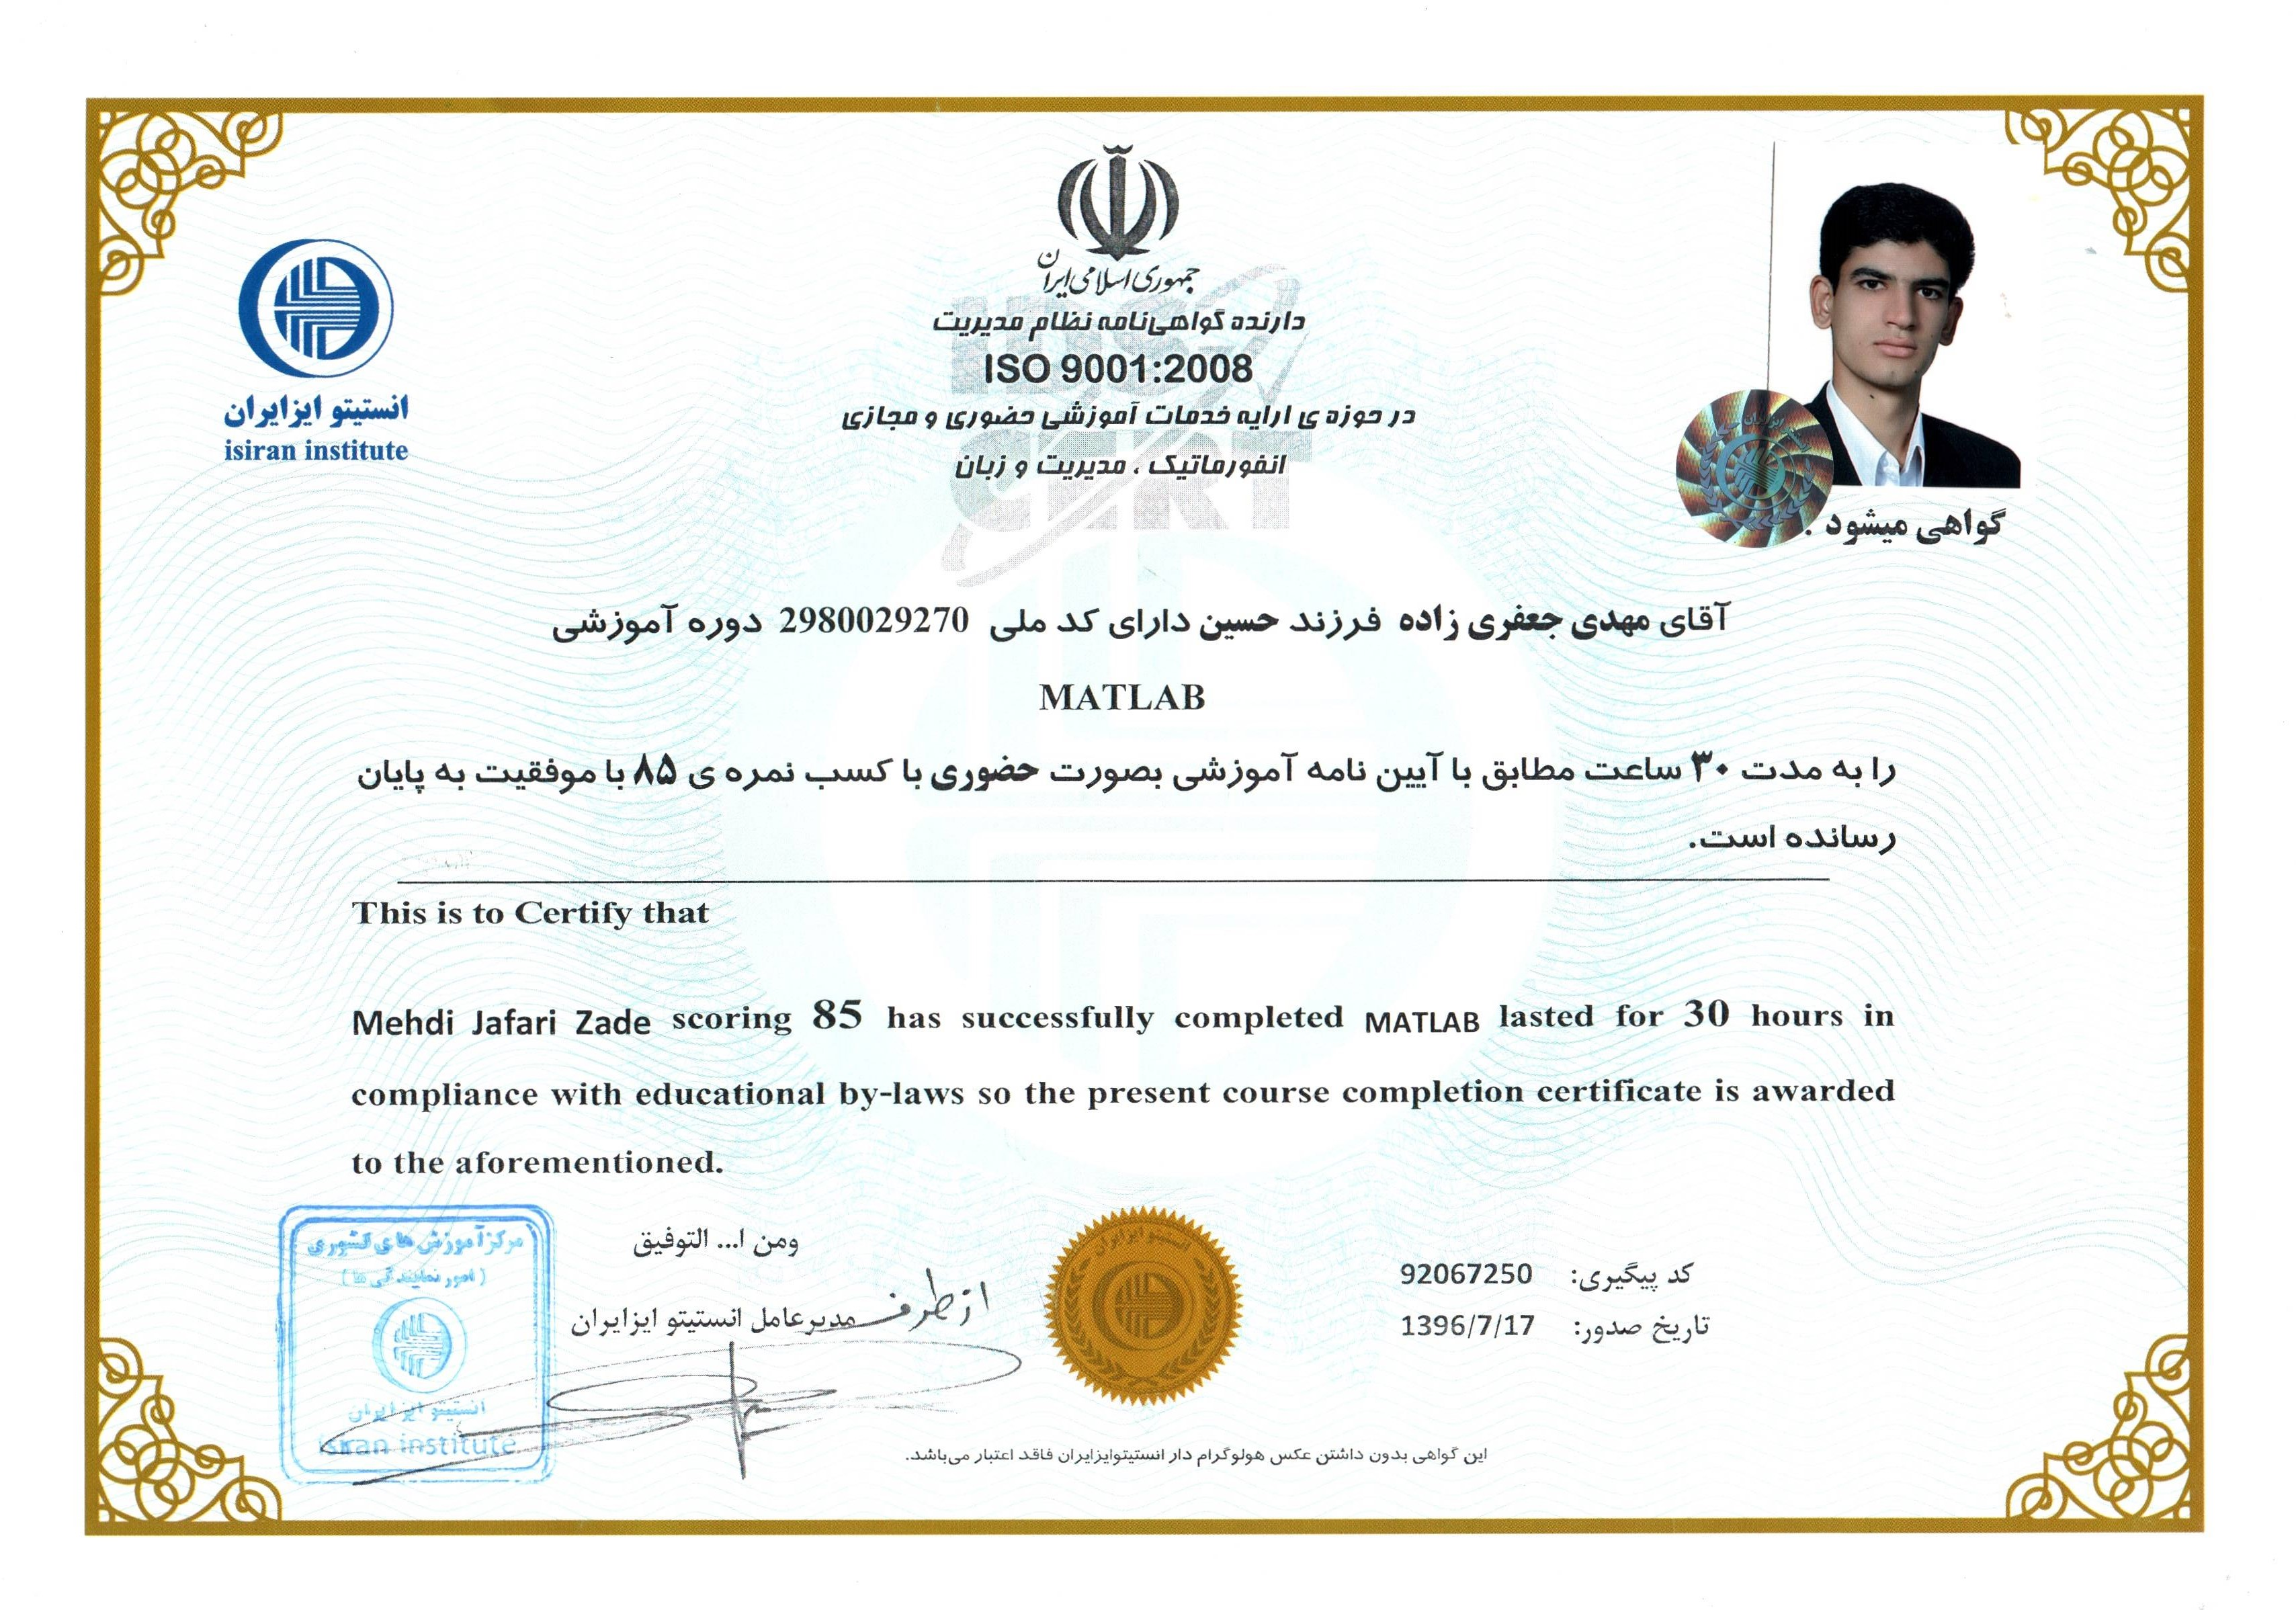
\includegraphics[width=\textwidth,height=\textheight,keepaspectratio]{../Document/Certificates of Achievement/MATLAB/09-10-2017 attestation de logiciel de MATLAB.jpg}
            \footnotesize
             \href{https://github.com/jafarizadeh/CV---lettre/tree/00df58c41988ba7488536512caee235bdb5d570d/Document/Certificates%20of%20Achievement/MATLAB}{Veuillez cliquer ici pour accéder au document sur GitHub}.
        \end{center}

    \newpage
    
    % 6.2 CCNA 200-301
    \subsection{CCNA 200-301}
    J'ai obtenu la certification Cisco Certified Network Associate (CCNA) avec un score impressionnant de 90, décernée par l'Institut d'Enseignement Supérieur Kherad en septembre 2024 et officiellement reconnue par le Ministère des Sciences. Ce programme rigoureux couvrait des domaines clés tels que les Fondamentaux des Réseaux, l'Accès Réseau, la Connectivité IP, les Services IP, les Fondamentaux de la Sécurité, ainsi que l'Automatisation et la Programmabilité. Ma solide performance dans ces domaines démontre une connaissance approfondie des architectures et des opérations réseau, me dotant de l'acuité technique nécessaire pour concevoir, implémenter et gérer des solutions réseau modernes.
     \newline
    \newline
        \begin{center}
            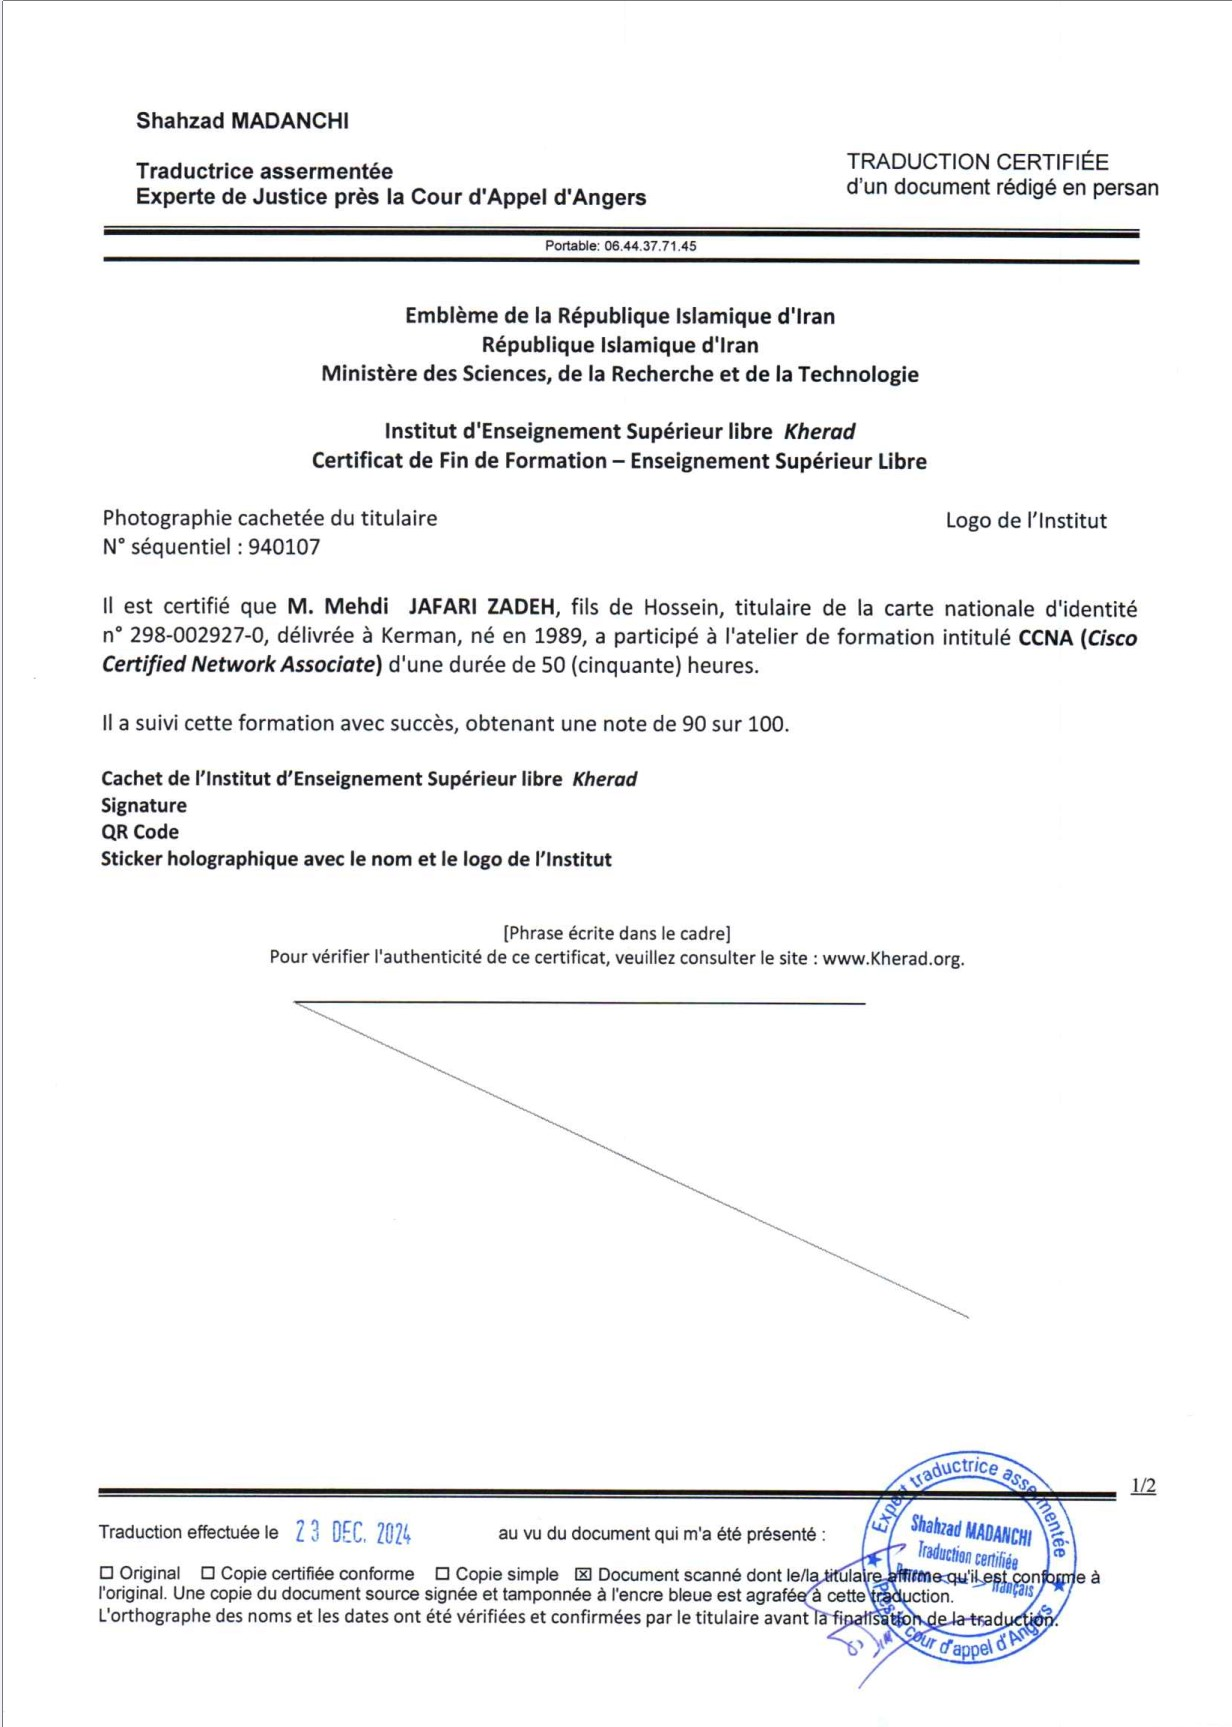
\includegraphics[width=\textwidth,height=\textheight,keepaspectratio]{../Document/Certificates of Achievement/CCNA 200-301/ccna.jpg}
            \footnotesize
             \href{https://github.com/jafarizadeh/CV---lettre/tree/903818f42bc563b419f3283c49cc84e05cf3932d/Document/Certificates%20of%20Achievement/CCNA%20200-301}{Veuillez cliquer ici pour accéder au document sur GitHub}.
        \end{center}
    \newpage



% =========================================================
% ============== Compétitions Scientifiques ===============
% =========================================================


\section{Compétitions Scientifiques}

    % 7.1 Design and manufacturing of wind turbines
    \subsection{Conception et Fabrication d'Éoliennes}
    J'ai obtenu la deuxième place au concours de conception et de construction d'éoliennes de 2016, organisé par l'Association Scientifique des Gènes de l'Énergie de l'Université de Technologie Moderne de Quchan. Le concours a mis au défi les participants de concevoir et de construire des modèles d'éoliennes innovants, en mettant l'accent sur la créativité, l'efficacité et l'application pratique dans les technologies des énergies renouvelables. Mon projet a été reconnu parmi de nombreuses soumissions pour son excellence en matière de conception et de fonctionnalité, démontrant ainsi ma compétence technique et mon approche innovante en ingénierie des énergies renouvelables.
    \newline
    \newline
    \textit {Note: Une image de la traduction Française de ce document est incluse dans les pages suivantes.}


    \newpage
    
        \begin{center}
            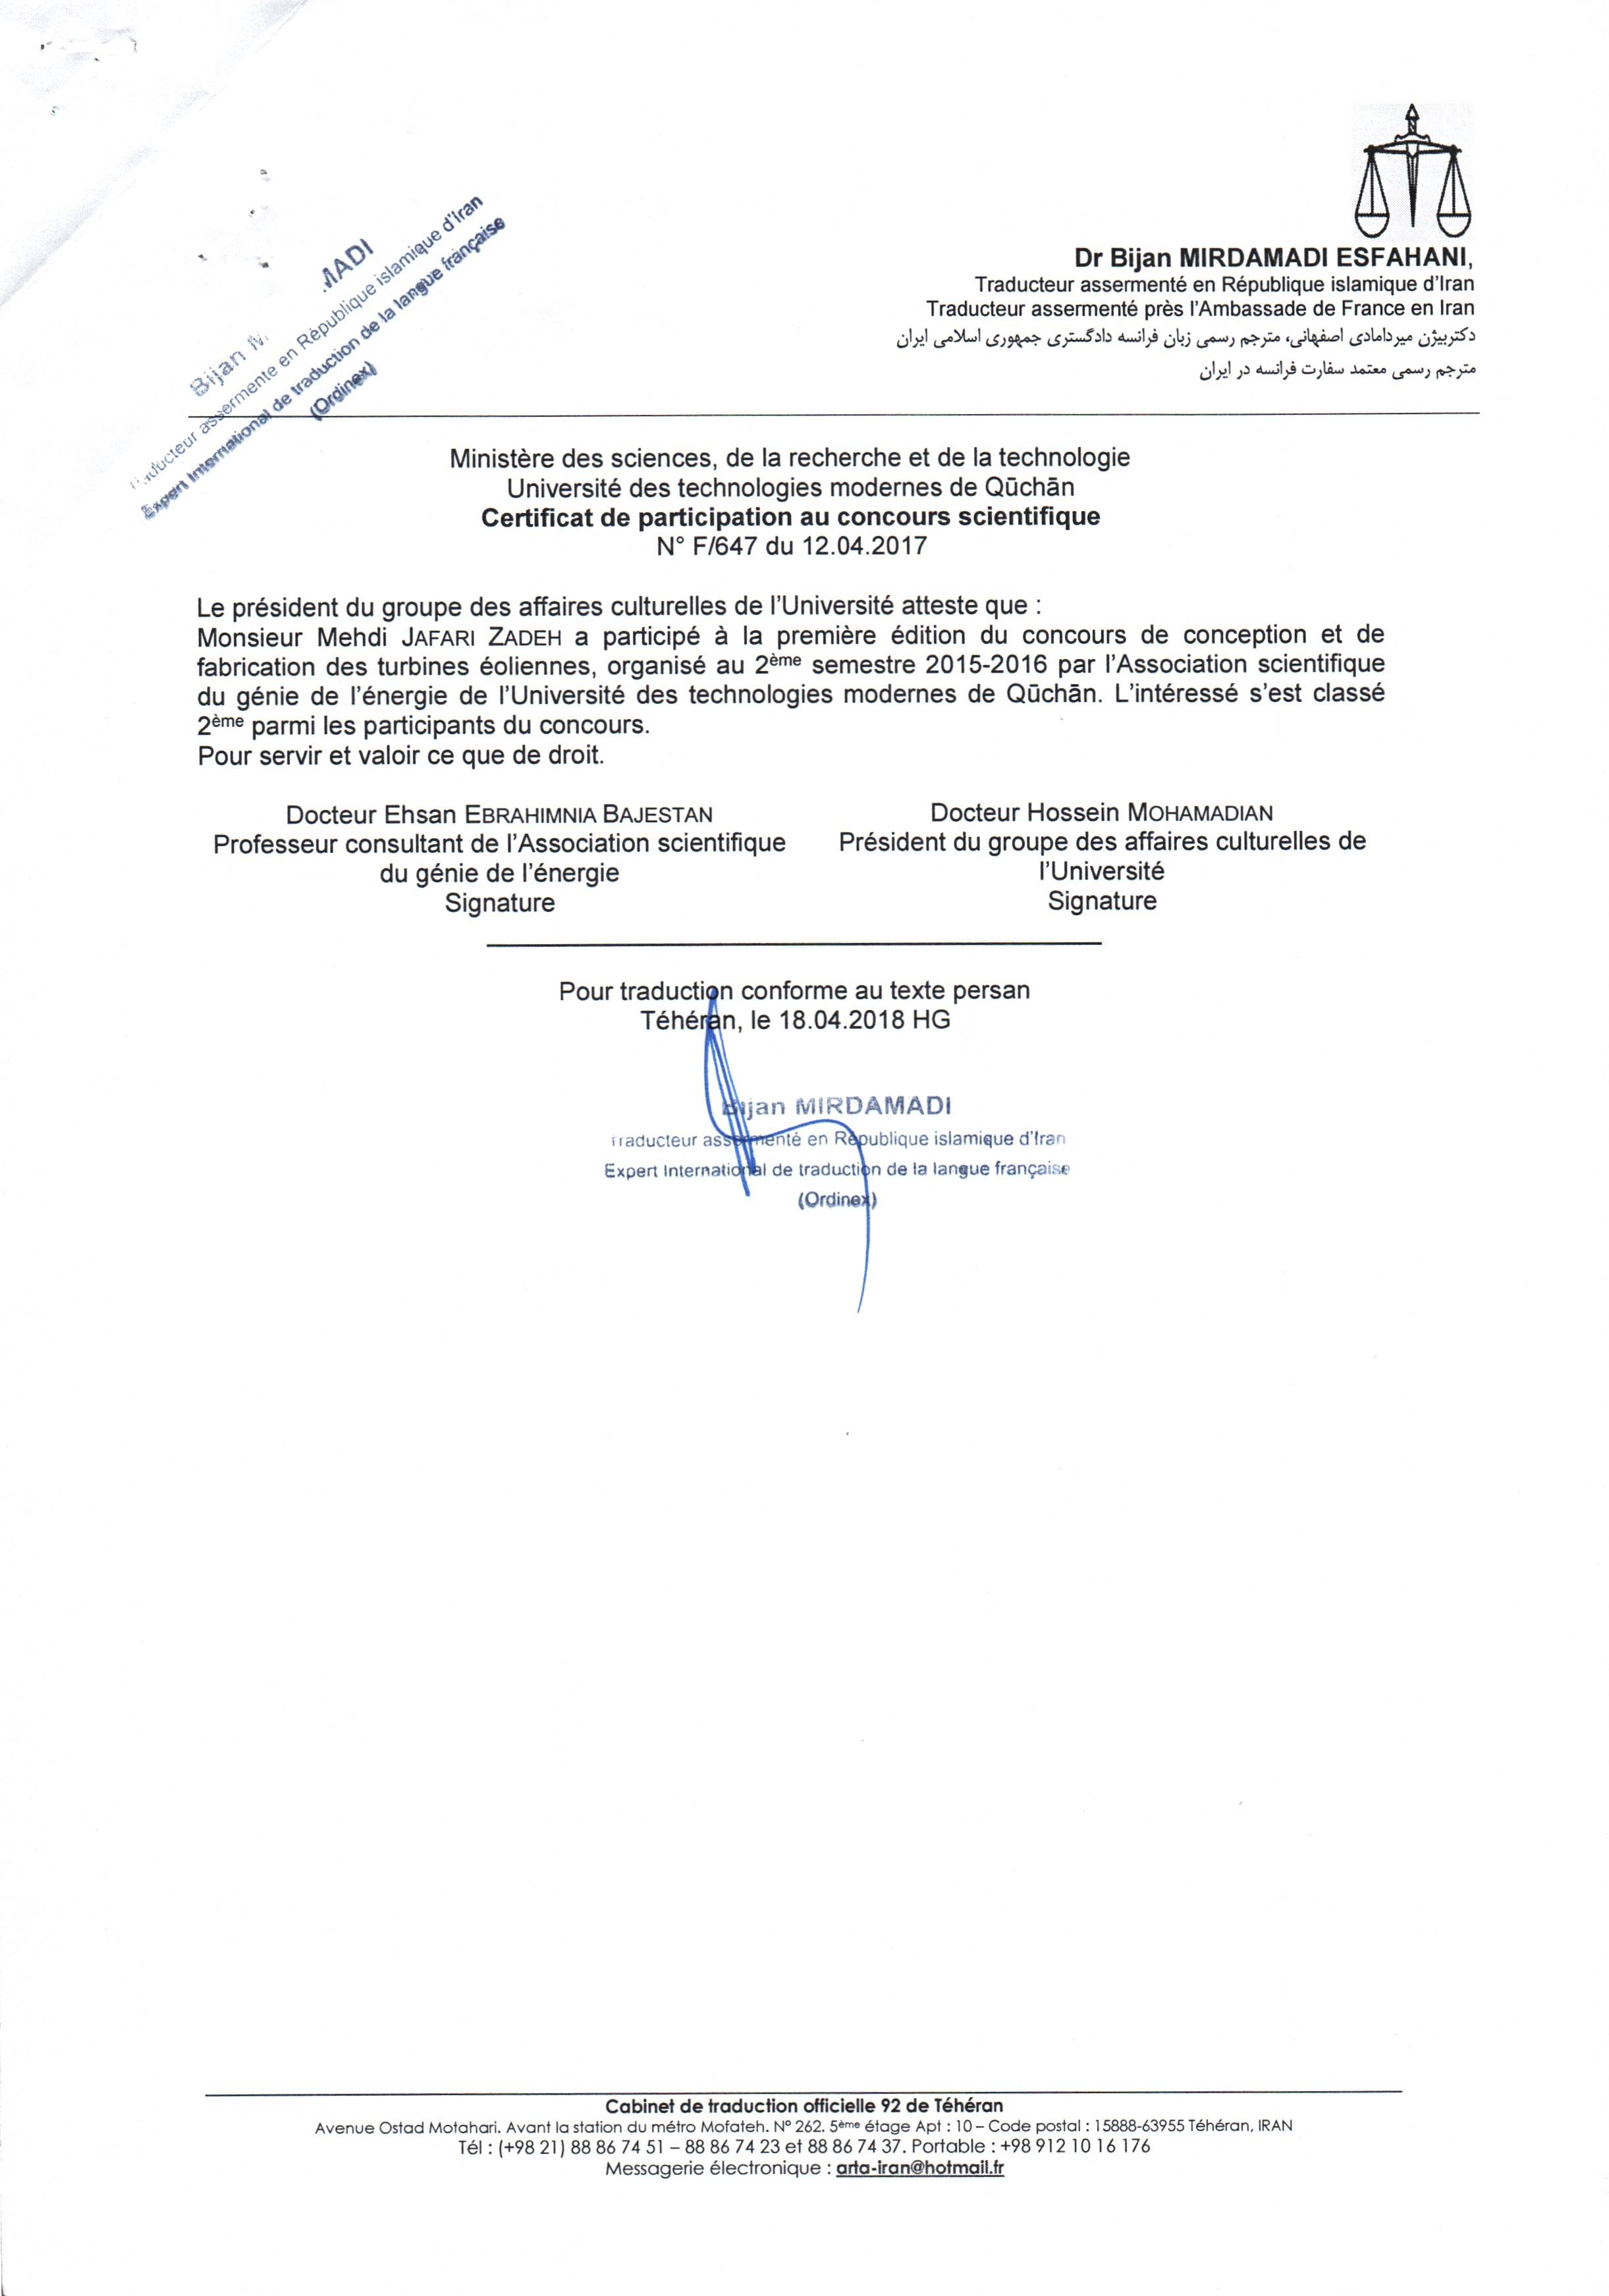
\includegraphics[width=\textwidth,height=\textheight,keepaspectratio]{7-1.jpg}
            \footnotesize
             \href{https://drive.google.com/drive/folders/1QJr8YZ-r2Zvn38sRTdmfIfaxAYCKjfNi}{Veuillez cliquer ici pour accéder au document sur GitHub}.
        \end{center}
    \newpage


% =========================================================
% ============= Certificat de Reconnaissance ==============
% =========================================================


\section{Certificat de Reconnaissance}

    % 8.1 Conférence du Professeur Soumchai Wangouiez
    \subsection{Conférence du Professeur Soumchai Wangouiez}
    En 2017, j'ai co-organisé et participé à une conférence scientifique de premier plan à l'Université de Technologie Moderne de Quchan. La conférence, dirigée par le Professeur Soumchai Wangouiez, était centrée sur le thème "Augmentation du Transfert de Chaleur par Écoulements Monophasés et Diphasés". Cet événement a constitué un rassemblement académique majeur qui a suscité des retours significatifs de la part de la communauté scientifique. Mon rôle consistait à collaborer avec une équipe d'étudiants et de professeurs universitaires pour faciliter les discussions et les présentations mettant en lumière les recherches innovantes et les avancées dans le domaine de l'ingénierie thermique. Cette expérience a non seulement approfondi ma compréhension des technologies de transfert de chaleur, mais a également renforcé mes compétences en matière d'organisation et de gestion d'événements académiques majeurs.
    \newline
    \newline
    \textit {Note: Une image de la traduction Française de ce document est incluse dans les pages suivantes.}
    \newpage
    
        \begin{center}
            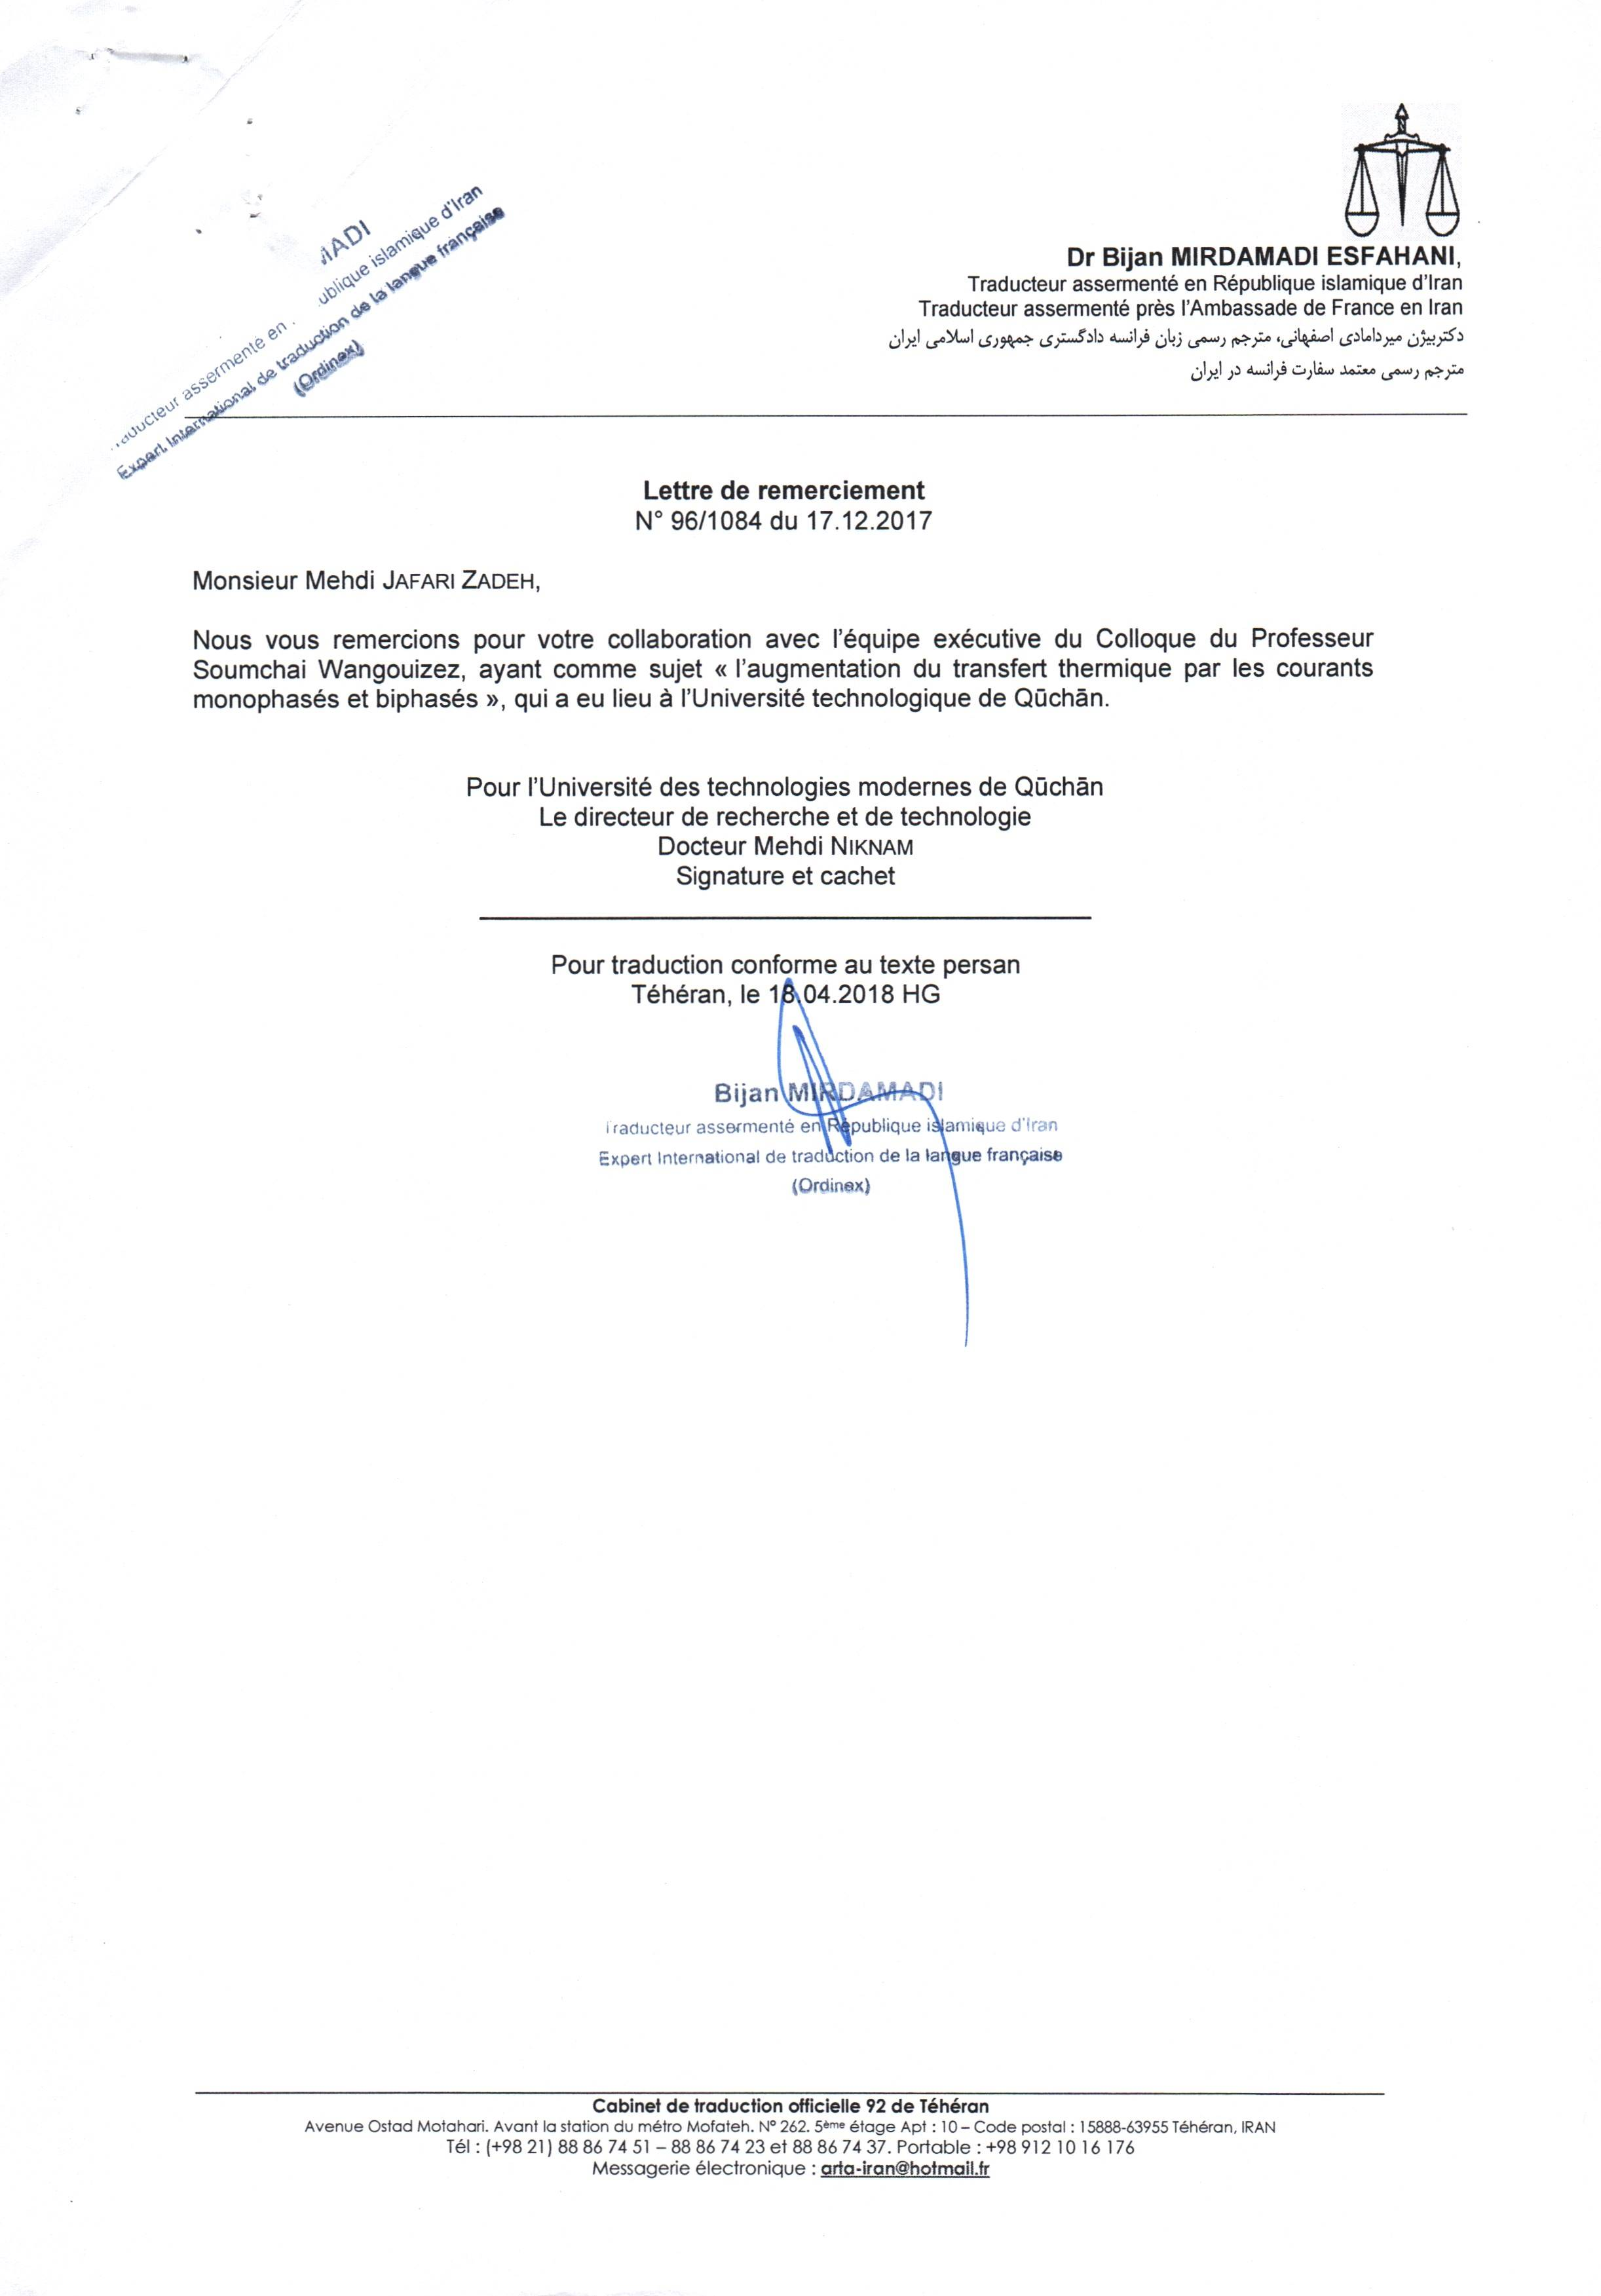
\includegraphics[width=\textwidth,height=\textheight,keepaspectratio]{8-1.jpg}
            \footnotesize
             \href{https://drive.google.com/drive/folders/1uKRDhC47KFOIxnGW9rlsWEyyyz1cDx7R}{Veuillez cliquer ici pour accéder au document sur GitHub}.
        \end{center}
    \newpage

    % 8.2 EES (Atelier Engineering Equations Solver)
    \subsection{Atelier EES (Engineering Equations Solver)}
    En 2018, à l'invitation du Dr. Morteza Anbarsooz, Professeur Assistant en Génie Mécanique à l'Université de Technologie de Quchan, j'ai animé un atelier sur le logiciel EES (Engineering Equation Solver) pour les étudiants de premier cycle. Cet atelier avait pour but de transmettre des compétences pratiques dans le calcul et la résolution d'équations complexes en énergie et en thermodynamique en utilisant EES. Ma capacité à communiquer efficacement ces concepts techniques a été reconnue par le Dr. Anbarsooz, qui m'a décerné un Certificat de Reconnaissance pour mon engagement à améliorer les connaissances des étudiants et à favoriser la croissance académique dans le domaine du génie mécanique.
    \newline
    \newline
    \textit {Note: Une image de la traduction Anglaise de ce document est incluse dans les pages suivantes.}


    \newpage
    
        \begin{center}
            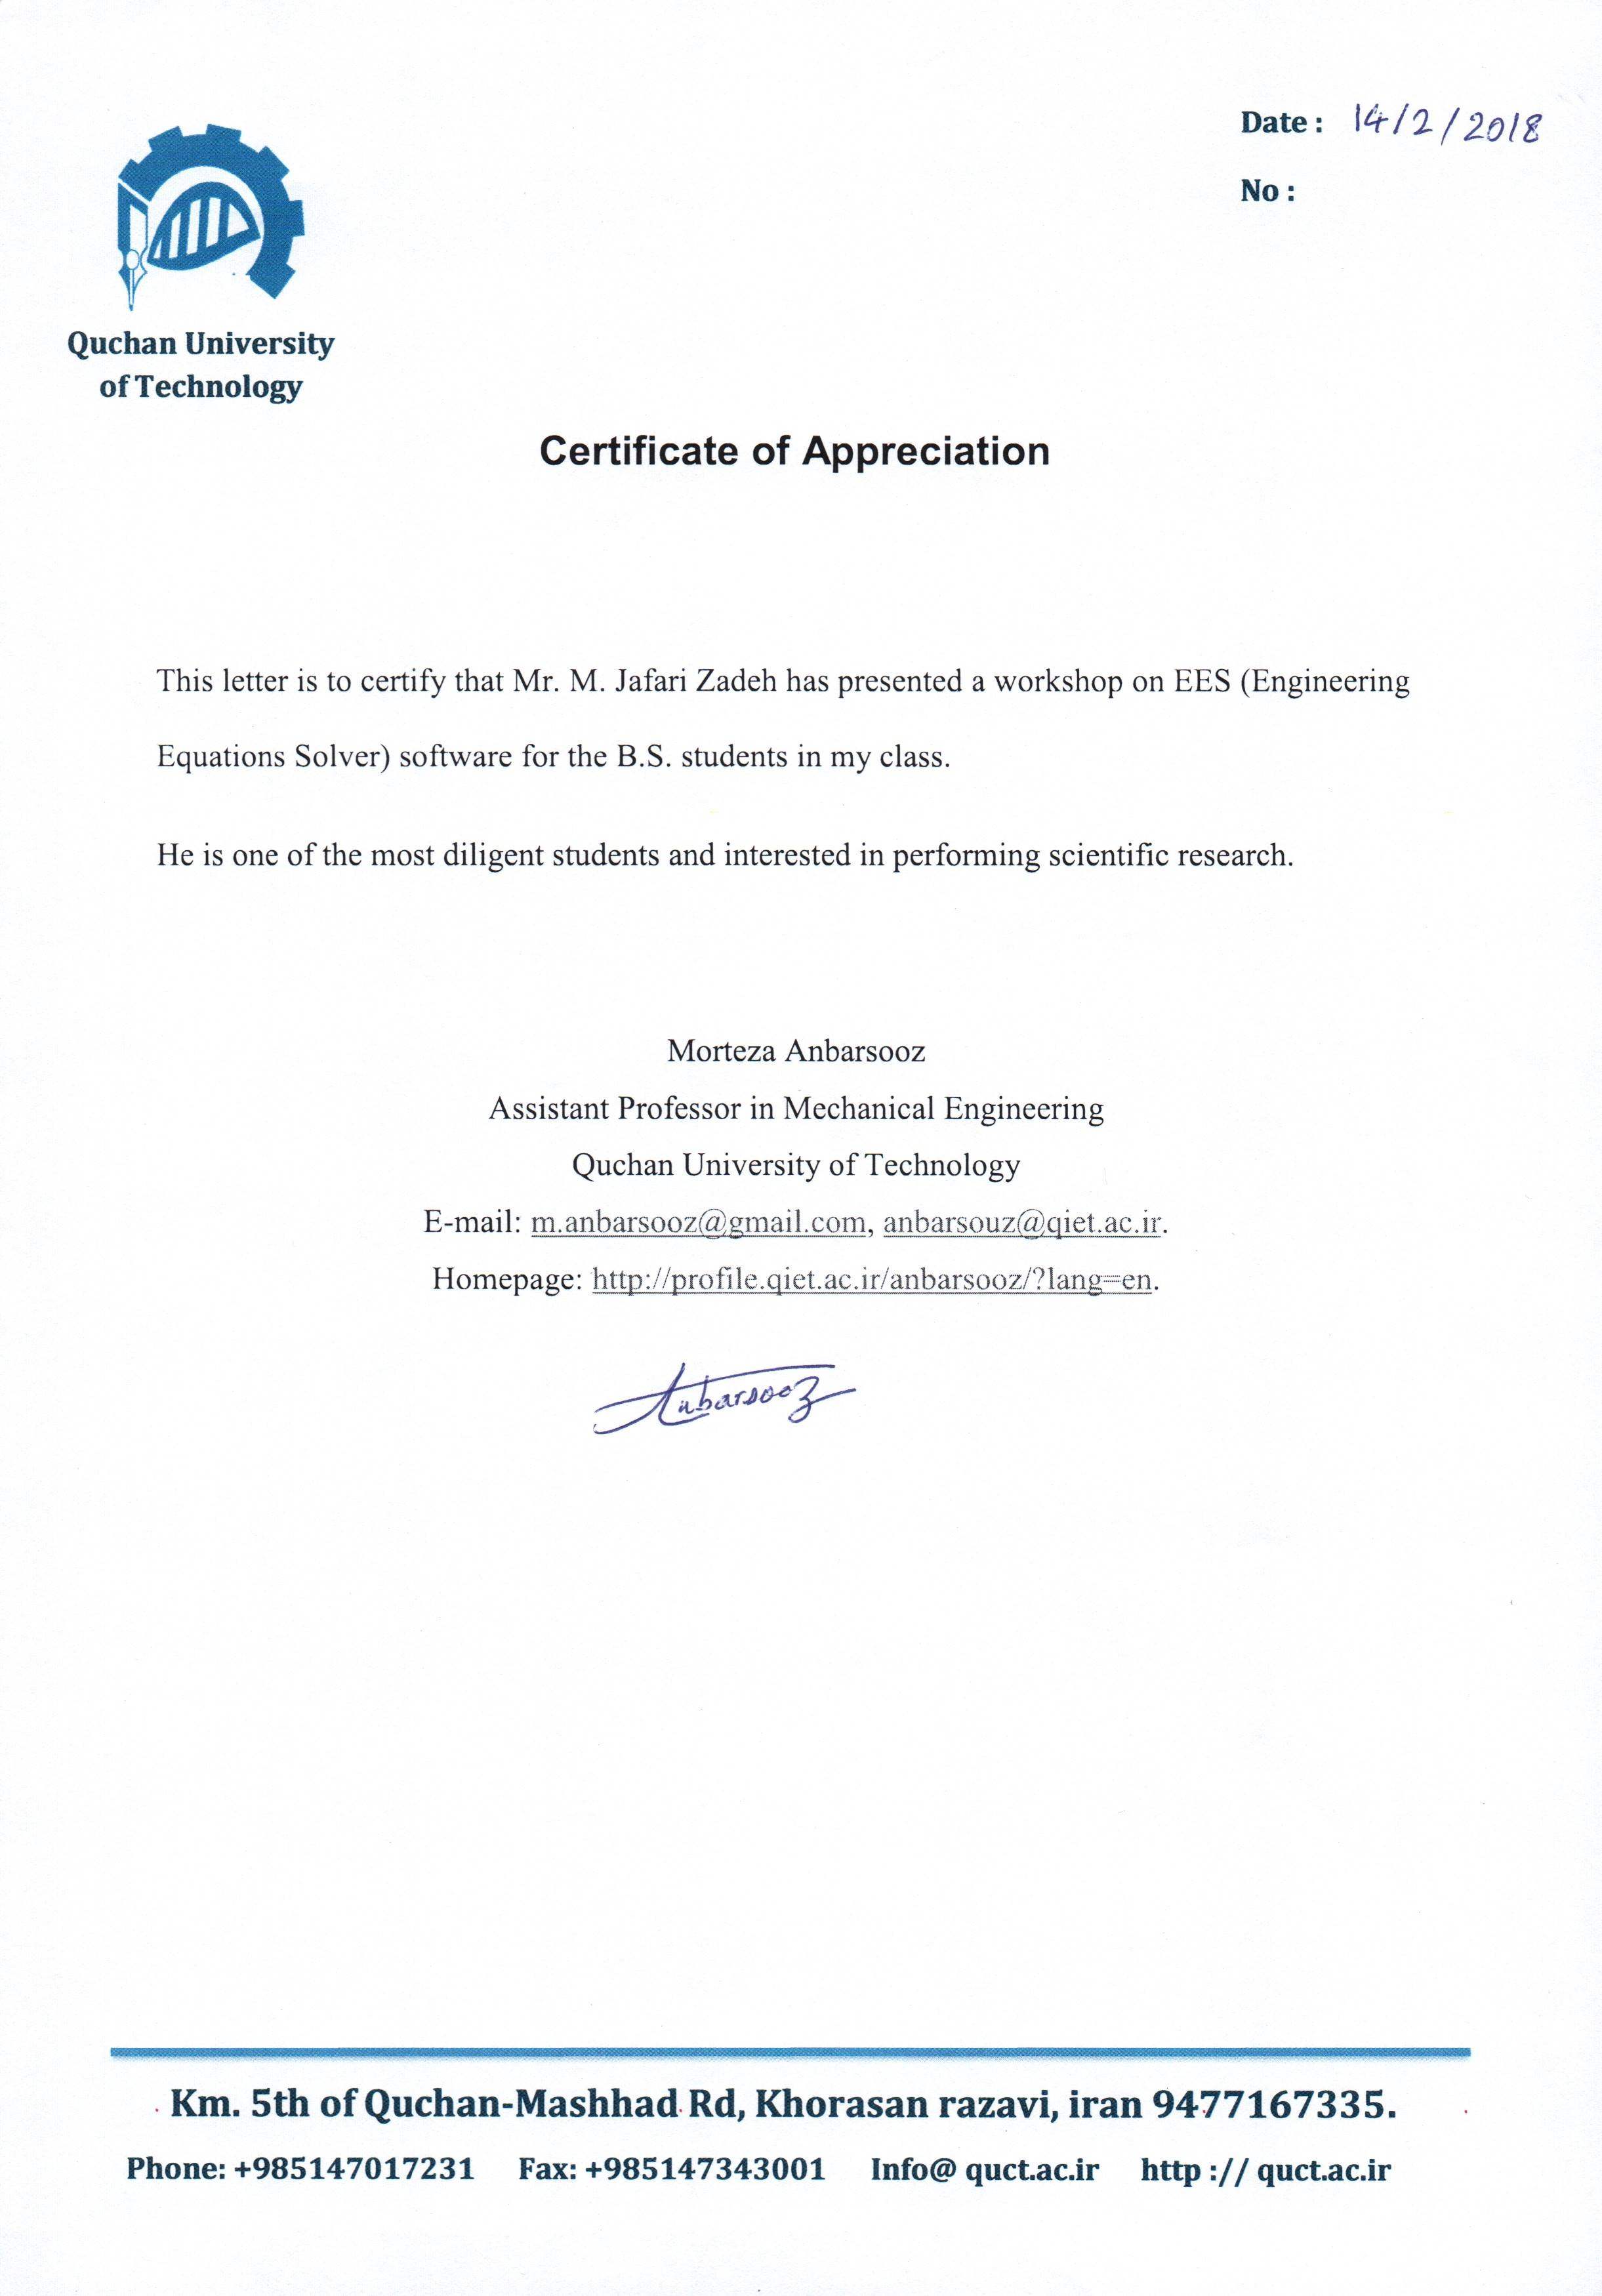
\includegraphics[width=\textwidth,height=\textheight,keepaspectratio]{8-2.jpg}
            \footnotesize
             \href{https://drive.google.com/drive/folders/1cAS8Ct20hDelABtksh8-BrusRfGzcSa3}{Veuillez cliquer ici pour accéder au document sur GitHub}.
        \end{center}
    \newpage


\section{Conclusion et Prochaines Étapes}

Alors que vous arrivez à la fin de ce portfolio, je voudrais résumer mes qualifications et mes aspirations futures. Mon objectif actuel est de faire progresser mes connaissances en informatique, en particulier dans le domaine du réseau, où je souhaite poursuivre un master. Cela approfondira davantage mon expertise et me préparera à une carrière en tant qu'administrateur réseau.

Mes études ciblées et mes certifications en réseau m'ont doté des compétences techniques nécessaires pour concevoir, gérer et sécuriser des infrastructures réseau complexes. Je suis désireux de me spécialiser davantage dans ce domaine grâce à des études avancées et de contribuer de manière significative à l'industrie.

Je suis ouvert à discuter de la manière dont mon parcours académique et mes compétences techniques peuvent correspondre à vos besoins, tant dans un cadre académique que professionnel. N'hésitez pas à me contacter à l'adresse \textbf{jafarizadeh89@gmail.com} ou au \textbf{0652224924}.

Pour des documents supplémentaires, veuillez y accéder via le lien suivant : \href{https://drive.google.com/drive/folders/1H4xCewHG2axnQZlIccB0N71s4JFHWjLJ?usp=drive_link}{[Lien vers les Documents Supplémentaires]}.

Merci d'avoir pris le temps de consulter mon portfolio. Votre considération est grandement appréciée.
\newline
\newline
Pour la version Anglaise de ce document, veuillez visiter \href{https://drive.google.com/file/d/1SwrSxWrC8iVVY-hpDYJElf16-4BYZWbR/view?usp=drive_link}{[Lien vers la Version Anglaise]}.

\end{document}
